\documentclass{xdupgthesis}

% XDUTS核心配置
\xdusetup{
  style = {
    customize-los = false,
    customize-loa = false,
  },
  info = {
    graduate-type         = 硕士,
    degree-type           = 专业,
    % 核心必填信息
    title                 = {面向单向双车道高速的多地磁传感器车辆目标跟踪方法研究},
    title*                = {Vehicle Target Tracking Using Multiple Geomagnetic Sensors on Unidirectional Two-Lane Highways},
    author                = {侯照莹},
    author*               = {Zhaoying Hou},
    department            = {通信工程学院},
    major                 = {信息与通信工程},
    major*                = {Information and Communication Engineering},
    sub-major             = {通信计算融合与场景应用},
    student-id            = {23011210459},
    supervisor            = {毛国强},
    supervisor*           = {Guoqiang Mao},
    supv-title            = {教授},
    supv-title*           = {Professor},
    supervisor-enterprise = {},
    supervisor-enterprise*= {},
    supv-ent              = {},
    supv-ent*             = {},
    supv-ent-title        = {},
    supv-ent-title*       = {},
    supervisor-title      = {教授},
    supervisor-title*     = {Professor},
    supervisor-enterprise-title  = {},
    supervisor-enterprise-title* = {},
    % 学科与保密信息
    domain                = {新一代电子信息技术（含量子技术等）},
    clc                   = {TP391.41},
    secret-level          = {公开},
    submit-date           = {2026-03-01},
    % 关键词
    keywords              = {车辆目标跟踪，地磁传感器，多目标跟踪，数据关联，在线聚类，轨迹重构},
    keywords*             = {Vehicle Target Tracking, Geomagnetic Sensor, Multi-Target Tracking, Data Association, Track Reconstruction},
    % 附件与声明文件
    abstract              = {chapters/abstract-zh.tex},
    abstract*             = {chapters/abstract-en.tex},
    acknowledgements      = {chapters/acknowledgements.tex},
    bio                   = {chapters/biography.tex},
    appendix              = {chapters/appendix1.tex},
    statement-scan        = {},
    statement-sign        = {},
    los                   = {chapters/los.tex},
    loa                   = {chapters/loa.tex},
    % 参考文献
    bib-resource          = {references.bib},
  }
}

% -------------------------
% 常用包（按功能分组）
% -------------------------
\usepackage{graphicx}
\graphicspath{{images/}}

\usepackage{amsmath}
\usepackage{amsfonts}
\usepackage{amssymb}

\usepackage{booktabs}
\usepackage{multirow}
\usepackage{makecell}
\usepackage{tabularx}
\usepackage{threeparttable}

\usepackage{subcaption}

\usepackage{xcolor}
\usepackage{pifont}

\usepackage{enumitem}


\usepackage{graphicx}
\graphicspath{{E:/MyLunWen/xduts-main/code/chapter4/experiment123/result/}}
 \usepackage{booktabs}
 \usepackage{float}

% 浮动体控制（你已在用：建议保留）
\usepackage[section]{placeins} % 提供 \FloatBarrier，并阻止浮动体跨 section
\usepackage{flafter}          % 防止浮动体出现在源码位置之前

% 超链接与智能引用：hyperref 必须在 cleveref 前面
\usepackage{hyperref}
\usepackage{cleveref}

% -------------------------
% 全局宏：模型名（你原本就有）
% -------------------------
\newcommand{\ModelTF}{GazeFusion}
\newcommand{\ModelMM}{GazeGuide}

% -------------------------
% 全局宏：地磁章节统一口径（按你第2章需要）
% -------------------------
\newcommand{\Fs}{\ensuremath{50\,\mathrm{Hz}}}
\newcommand{\MagUnit}{\ensuremath{\mathrm{nT}}}
\newcommand{\SmoothLen}{\ensuremath{7}}        % L_s
\newcommand{\BgWinPts}{\ensuremath{500}}       % N_0 (10 s @ 50 Hz)
\newcommand{\ProbFloor}{\ensuremath{10^{-6}}}  % p_min

% 兜底：即使 placeins 被注释掉，也不至于 \FloatBarrier 报错
\providecommand{\FloatBarrier}{}

% -------------------------
% 文档开始
% -------------------------
\begin{document}


\chapter{绪论}

\section{研究背景与意义}

近年来，随着跨区域人员流动日益频繁和公路货运需求持续增长，高速公路在综合交通运输体系中的支撑作用不断增强。交通运输部数据显示，截至2024年末我国高速公路里程已达19.07万公里\cite{mot2024statisticalbulletin}，路网规模的持续扩展也使高速公路运行管理由单纯保障通行，逐步转为面向安全、效率与韧性的精细化治理。尤其在高速场景下，车辆运行速度高、交通流密度大、扰动传播快，局部异常往往会迅速影响车道乃至路段整体运行状态。因此，如何构建实现面向高速路段的持续感知与精细管理能力，已成为保障路网安全高效运行、提升运行韧性并支撑主动交通管理的重要基础问题。

在此背景下，智能交通系统（ITS）通过交通检测与监视、通信与信息处理等技术实现对交通状态的实时感知与服务支撑，从而为交通管理与控制提供数据基础\cite{mimbela2007vdstits}。交通治理也逐渐由以流量、平均速度等宏观统计指标为主逐步转向车道级运行机理与驾驶行为的微观刻画。相应地，能够连续描述车辆时空运动过程的轨迹数据成为交通分析、预测与控制的关键数据形态\cite{liu2025trajectorysurvey}，并可用于拥堵成因诊断、行驶安全风险与冲突指标计算、以及车路协同控制策略评估等任务。然而，这类轨迹数据并非由路侧传感器直接输出，而是需要对离散检测结果进行时序组织、状态估计与身份维护后才能形成，车辆目标跟踪正是实现这一过程的关键技术。车辆目标跟踪的任务，是将路侧传感器输出的离散检测结果或量测序列在时间轴上进行一致性组织与身份维护，形成可持续更新、可用于实时管理与控制的车辆轨迹；同时在车道级应用中尽量保持位置与速度估计的连续性，为上层行为分析提供可靠输入，以支撑车道级速度估计、时距演化分析与变道行为识别等应用。需要指出的是，车辆目标跟踪的实施效果高度依赖路侧感知载体的观测能力与工程可用性，不同类型传感器在目标分辨能力、环境适应性以及部署维护成本等方面各有特点，这也决定了其在高速公路场景中的适用边界。以常见路侧传感器为例，摄像头能够提供丰富的轮廓、纹理与颜色信息，但在强逆光、夜间、雨雾等条件下检测质量易波动\cite{Pandharipande2023Perception}；激光雷达空间分辨率高、测距精度较好，但设备成本较高，且在降雨、降雪等天气下点云质量可能受到影响\cite{Pandharipande2023Perception,Wu2025LiDARAdverseWeather}；毫米波雷达对光照不敏感，在恶劣天气下相对更稳健，但在强多径环境中仍可能出现虚假检测，且受角分辨率限制，对邻近目标的分离能力仍存在约束\cite{Kong2025mmWaveSurvey}。 

在面向大范围、全天候部署的路侧感知体系中，地磁传感器因成本较低、体积小、安装灵活且对光照与气象条件不敏感，被认为是面向低成本规模化部署的关键候选方案，其基本机理是车辆等铁磁体通过时会扰动局部地球静磁场，传感器对磁场变化进行采样与特征提取，从而输出车辆通过事件及相关磁特征\cite{culik2023wirelessmagnetic}。不同于能够直接给出连续轨迹的感知方式，在多地磁传感器组网条件下输出的是跨位置的离散检测数据流，这些数据需要在时间轴上对齐，并在多车并行与变道交互条件下完成跨点匹配与身份维护，才能转化为可用于微观分析的连续轨迹。然而在实际部署中，多地磁传感器跟踪系统存在数据随机延迟到达、漏检以及噪声干扰等非理想因素的影响，同时由于车辆行驶行为复杂，邻道干扰与双车长距离并行通过在上报量测的时空特性上又具有较强相似性，难以简单依据单条量测特征判断区分，从而影响车辆实时跟踪的准确性与稳定性。进一步地，系统连续多年使用后，部分地磁传感器还可能因器件老化而检测能力下降，连续漏检现象增多，使跟踪结果更易出现轨迹碎片化\cite{rakai2022dataassociation,feng2021magneticdataassociation,wang2023distributedmagnetic}。由此可见，如何在不完美量测条件下实现多地磁事件流的稳健在线跟踪，并在长缺测条件下进一步恢复断裂轨迹片段、保持轨迹身份一致性，是释放地磁传感在高速运行监测中应用价值的关键技术问题，也对轨迹级安全评估与精细化交通管理具有重要意义。

\section{国内外研究现状}

\subsection{地磁传感器车辆检测研究现状}
地磁传感器是一种基于环境磁场变化的路侧检测设备，通常采用磁阻器件对周围磁场进行连续采样。当车辆驶过传感器附近时，车辆所含铁磁材料会对局部磁场分布产生扰动，使磁信号在幅值与形态上出现显著变化；对该扰动信号进行检测与判别即可实现车辆通过事件的识别\cite{balid2018intelligent,feng2022magmonitor}。

早期研究以单点车辆检出与过车片段起止时刻提取为基础。Haoui等以无线地磁检测网络VDS240为例，展示了节点端完成检测后上报检测记录、再由中心侧汇聚处理的系统形态，并进一步指出在单车检测记录层面可计算速度、占有率、车长以及车头时距等指标\cite{haoui2008wirelessmagnetic}。在算法与误差机理层面，Markevičius等提出基于状态判据的车辆检测思路，并指出车辆通过地磁传感器的轨迹差异会显著改变小型地磁传感器记录到的扰动波形形态，因此在检测输出生成时通常需要考虑归一化与自适应处理，以减弱同车不同通过轨迹带来的特征漂移\cite{markevicius2016dynamic}。随着检测可靠性逐步提升，研究开始将单点检测记录用于交通参数估计与分类。Taghvaeeyan与Rajamani构建可路侧布设的磁传感系统，利用纵向布设传感器的互相关估计速度，并结合占有率与速度推断车辆磁长度，同时通过磁场模型抑制邻道大型车辆造成的误触发\cite{taghvaeeyan2014portable}。Balid等进一步把车辆检测、速度估计、长度估计、车辆分类以及时钟同步算法集成于智能无线传感器并开展实地评估，反映出检测输出能力正向端侧实时一体化并引入同步机制的方向演进\cite{balid2018intelligent}。为增强单点输出的可解释性与稳定性，Feng等提出MagMonitor，通过多磁偶极车辆磁场模型实现单传感器速度估计与车辆分类，说明模型化描述有助于在检测输出阶段提取更稳定、更可解释的特征\cite{feng2022magmonitor}。当研究进一步扩展到阵列观测时，Amodio等利用路面多传感器记录车辆不同部位的多段磁签名，并采用动态时间规整实现车辆型号识别与横向通过位置估计，表明空间采样能够支撑车道尺度的更细粒度刻画\cite{amodio2021vehiclemodel}。在跨空间连接方面，Kwong等构建基于无线地磁签名匹配的实时旅行时间估计框架，利用带噪磁签名与过车时刻在两点间进行重识别并估计旅行时间分布，验证了地磁检测记录与签名具备跨点复用的匹配价值\cite{kwong2009arterialtravel}。然而，当系统从单点走向多点组网并进入双车道场景后，不完美观测会显著放大跨点对应难度。Feng等指出多地磁传感器之间的时钟偏差与换道会引起量测时标错位及漏检与重复检出，但其提出的组网关联方法以检测统计为导向、场景假设较强，难以保证高速双车道密集车流下轨迹精度与ID连续性\cite{feng2021magneticdataassociation}。Mao等进一步面向随机延迟与不准确检测讨论异步融合机制，并在融合毫米波雷达与地磁量测的场景中验证了方法有效性；但对于仅依赖地磁量测、且量测可能出现更长缺失的低成本高速路侧部署条件，上述思路难以直接覆盖在线跟踪需求\cite{mao2025asynchronousfusion}。

综上，现有研究已能在单点层面稳定输出车辆检测量测，并进一步派生速度、占有率与车长等参数；在阵列观测条件下，还可获得车道级属性并提取可用于跨传感器匹配的磁签名。然在双车道密集交通的多地磁传感器组网场景下，基线漂移与噪声时变、节点间时钟偏差及随机通信延迟叠加漏检与虚警，造成的量测时序不一致、漏检与多检等问题，仍缺乏有效的系统性解决方案。因此，在量测存在噪声干扰、时序不一致与漏检并存条件下实现多车辆的实时、准确跟踪，并兼顾轨迹精度、连续性与身份一致性，仍是亟待解决的关键问题。

\subsection{滤波算法研究现状}
滤波算法是多目标跟踪中实现状态预测与更新的基础。对于本文关注的高速路侧多地磁传感器车辆目标跟踪场景，滤波结果不仅决定车辆位置、速度等状态量的估计精度，也会进一步影响后续的数据关联与轨迹维护。从研究脉络来看，相关方法大体经历了从线性平稳过程到线性动态系统，再到非线性、机动与非高斯场景的逐步扩展。最早可追溯到 Wiener 于 1949 年提出的平稳随机过程最优线性滤波理论\cite{wiener1949extrapolation}。该理论奠定了现代滤波方法的数学基础，但其求解仍较多依赖 Wiener-Hopf 方程，对非平稳统计和复杂动态系统的推广并不方便。随后，Kalman 于 1960 年从状态空间和状态转移的角度重新表述滤波与预测问题，提出了 Kalman 滤波算法\cite{kalman1960linearfiltering}。与 Wiener 滤波相比，Kalman 滤波能够以递推方式完成预测和更新，更适合实时状态估计，因此很快成为目标跟踪领域线性系统状态估计的经典方法。

随着跟踪对象由近线性目标扩展到更复杂的机动目标，20 世纪 60 年代中期以 Schmidt 为代表的研究开始将状态空间方法系统应用于导航等非线性问题，并逐步形成围绕一阶线性化的扩展卡尔曼滤波思路\cite{schmidt1966statespace}。EKF 的基本思想是在当前估计点附近对非线性状态方程和量测方程作 Jacobian 线性化，再沿用 Kalman 滤波的递推结构完成状态估计。由于其实现形式与 KF 较为接近，工程应用比较广泛；但当系统非线性较强或模型失配较明显时，线性化误差容易积累，进而导致估计精度下降，严重时甚至出现发散。进一步地，针对机动目标模型切换问题，Blom 和 Bar-Shalom 于 1988 年提出了交互式多模型算法 IMM\cite{blom1988imm}，通过并行运行多个运动模型并对模型概率进行交互融合，有效缓解了单一运动模型难以刻画加减速、转向或变道等机动行为的问题，这也使其在车辆目标跟踪中具有较强的适用性。

进入 20 世纪 90 年代以后，非线性滤波研究继续沿两条路线展开。一方面，Gordon 等于 1993 年提出了 bootstrap particle filter，用带权粒子来近似系统状态的后验分布，使滤波过程不再受线性和高斯假设的严格限制\cite{gordon1993bootstrap}。该方法能够处理更一般的非线性、非高斯问题，但也容易受到粒子退化的影响，并且为保证估计精度通常需要较多粒子样本，从而带来较高的计算代价。另一方面，Julier 和 Uhlmann 在 1997 年提出 UKF，并在 2004 年对无迹变换和无迹滤波进行了系统总结\cite{julier1997ukf,julier2004unscented}。UKF 通过选取确定性的 sigma 点传播均值与协方差，避免了 EKF 中显式求 Jacobian 的过程，在不少非线性场景下较好地兼顾了实现便利性与估计精度。不过，其本质上仍是基于有限统计量对后验分布进行近似。总体来看，滤波算法的研究主线已经从早期面向平稳过程的线性最优估计，逐步发展为兼顾非线性、机动模型切换以及非高斯噪声的状态估计框架。对于本文所研究的高速路侧多地磁传感器车辆目标跟踪问题而言，车辆运动模式会随交通状态变化，量测又易受环境扰动与漏检影响，因此如何在保证实时性的同时兼顾机动性描述与估计稳定性，仍然是滤波算法设计中的关键问题。

\subsection{数据关联研究现状}
与单目标场景不同，多目标跟踪中的核心难点之一在于量测归属不确定性。滤波预测只能为每条轨迹给出先验分布，而当前时刻的量测应由哪一条轨迹吸收更新，需要通过数据关联判定；一旦发生错误关联，错误量测会进入状态更新，并引发状态漂移与ID切换，并在递推中持续放大\cite{barshalomli1995multitarget}。

在早期研究中，Singer与Stein已关注量测来源不精确条件下的跟踪滤波问题，指出关联不确定性会显著影响递推估计的稳定性与可信度\cite{singer1971optimaltracking}。为降低候选匹配数量，工程中通常先依据预测均值与协方差等构造一个验证门（即门控），以剔除明显不可能的匹配；在此框架下，Sea提出实时监视系统的次优关联决策过程，采用门控内最近邻量测进行更新，后续被概括为最近邻数据关联（Nearest Neighbor Data Association, NNDA）\cite{sea1971suboptimal}。但在密集交通与变道交互下，多个验证门易重叠，单一扫描的最近邻选择更易误配。

确定性数据关联在每一帧输出唯一的一一匹配。典型代表包括NNDA及其全局化形式全局最近邻（Global Nearest Neighbor, GNN），即在门控后的候选集合上求解指派问题以获得整体代价最小的匹配。Kuhn提出的匈牙利算法是GNN常用的指派求解器\cite{kuhn1955hungarian}。该类硬判决方法实现简单、计算量小，但在量测拥挤时一旦误配往往难以自纠，ID切换风险上升。为降低硬判决错误匹配带来的冲击，Bar-Shalom与Tse提出概率数据关联（Probabilistic Data Association, PDA），对验证门内候选量测计算关联概率并加权更新\cite{barshalom1975pda}；Fortmann等扩展得到联合概率数据关联（Joint Probabilistic Data Association, JPDA），通过联合关联事件的概率化处理缓解多目标争抢量测导致的轨迹黏连\cite{fortmann1983jpda}。针对在线复杂度约束，国内研究提出广义概率数据关联与简化JPDA等近似形式，以减少联合事件枚举开销并提升可用性\cite{pan2005gpda,qin2005simplifiedjpda}，简化JPDA也被用于密集杂波条件下的稳健跟踪\cite{sheng2020simplifiedjpda}。

单扫描关联的局限在于早期误配会改变后续门控结构并产生链式传播。多扫描方法在有限时间窗口内综合多帧证据进行联合决策或后验校正：Reid提出多假设跟踪（Multiple Hypothesis Tracking, MHT）以并行维护多套关联假设\cite{reid1979mht}，Cox与Hingorani给出高效实现并强调剪枝对实时性的关键作用\cite{cox1996efficientmht}；Murty算法用于生成多组候选指派\cite{murty1968ranking}，网络流、贪心与K最短路等全局优化框架可用于多帧轨迹连接\cite{zhang2008networkflow,pirsiavash2011greedy,berclaz2011kshortest}。在在线应用中，多扫描方法通常结合固定滞后窗口与近似求解，将计算复杂度控制在可承受范围内并获取跨帧一致性收益。关于MHT的长期发展脉络，Chong等对四十年研究进展进行了专门综述\cite{chong2019forty}。

\subsection{在线轨迹聚类方法研究现状}
与前述侧重递推滤波与在线关联不同，本节关注当观测出现较长中断或连续缺测时，在线跟踪输出往往分解为多个短轨迹片段，从而出现轨迹碎片化现象。在此背景下，研究重点由单次量测更新转向跨片段的一致性组织，即将轨迹点或轨迹片段作为聚类对象，利用时空邻近与运动一致性线索对同一目标的片段进行增量聚合与归并，以在更长时间尺度上提升轨迹连续性与身份一致性\cite{wang2021trajectorysurvey,wang2024reconstruction}。

从聚类的一般方法出发，密度聚类常被用作基础工具。DBSCAN以密度可达性定义簇结构，能够发现任意形状的簇，并将低密度样本识别为噪声点，因此在噪声与离群点并存的数据中具有较好的结构分离能力\cite{ester1996dbscan}。不过，DBSCAN主要面向静态数据集，难以直接满足数据流场景中一次扫描、有限存储与持续到达的处理约束。面向数据流聚类，CluStream将在线阶段的微簇维护与离线阶段的宏聚类分析相分离，通过维护可更新的统计摘要支持不同时间尺度上的聚类查询，为流式数据的可扩展聚类提供了经典范式\cite{aggarwal2003clustream}。在此基础上，DenStream进一步引入核心微簇、潜在微簇与离群微簇等结构，并结合剪枝策略实现对噪声与演化簇结构的在线处理，使聚类过程在数据分布随时间变化时仍能保持跟踪性与稳健性\cite{cao2006denstream}。总体来看，上述工作形成了由静态密度聚类向演化数据流聚类拓展的基础框架，为后续将轨迹样本视为数据流并进行增量归并提供了方法论支撑。

进一步面向轨迹数据，已有研究指出仅依赖通用点集聚类往往不足以刻画轨迹数据中蕴含的时序信息与运动一致性，从而难以稳定完成片段归并。为此，研究者提出面向轨迹数据流的在线聚类方法，将轨迹点序列转化为具有时序语义的表示单元并进行增量组织。Yu等提出CTraStream，将移动对象的增量轨迹表示为线段流，并结合线段间距离度量与在线更新机制，在流式到达过程中持续形成包含时空信息的轨迹簇，为轨迹数据流的实时模式提取提供了可操作框架\cite{yu2013ctra}。Mao等进一步针对流式轨迹的概念漂移与时空开销约束提出OCluST，通过微聚类与宏聚类两级结构在给定时间跨度内维护轨迹簇，使聚类结果能够随轨迹模式演化而更新，体现了时间窗口内增量聚合的轨迹流聚类思路\cite{mao2018oclust}。此外，面向轨迹重建与行为一致性约束的研究也在持续推进\cite{zhao2024behaviouraloc}。然而，当数据呈现长间隔缺测、目标数量动态变化时，现有在线轨迹聚类方法仍难同时兼顾簇结构的稳定维护与误聚类抑制。




\section{论文研究内容及章节安排}

本文的研究内容是将多地磁传感器车辆检测与目标跟踪技术相结合，面向单向双车道高速路段的地磁检测数据，实现多车辆在线跟踪并输出连续、身份一致的车辆轨迹。全文安排如下：

第一章为绪论，阐述高速公路运行监测与微观过程管控需求，概述地磁感知与车辆跟踪研究现状，明确本文研究问题、技术路线与创新点。
第二章给出单向双车道多地磁布设与量测建模，并介绍车辆检测与事件生成、状态空间模型、贝叶斯递推、门控与数据关联以及轨迹重构相关基础概念，为后续方法推导统一符号与假设。

第三章面向噪声统计不确定、短时漏检与密集交通下的关联歧义，提出变分贝叶斯噪声自适应滤波结合门控与软关联的在线多目标跟踪方法，并给出算法流程与性能分析。

第四章面向连续缺测引发的轨迹碎片化问题，设计基于聚类的轨迹重构策略，对跟踪输出进行二级整合并验证其有效性。第五章总结全文工作与主要结论，讨论研究局限并展望后续改进方向。





\chapter{多地磁传感器车辆目标跟踪理论概述}
\label{ch:ch2_event_detect}

\section{引言}\label{sec:ch2_intro}

在前述研究背景与相关工作综述的基础上，本章围绕单向双车道多地磁传感器部署场景下的车辆目标跟踪问题，对相关理论与部署模型进行系统阐述。具体而言，首先介绍地磁传感器的车辆检测机理及事件生成过程；随后给出本文所采用的系统部署模型及其对应的测量模型；在此基础上，对卡尔曼滤波与数据关联的基本理论进行回顾，并进一步梳理在线聚类算法的相关方法，为后续章节的算法设计与推导奠定理论基础。


\section{地磁传感器检测车辆}\label{sec:ch2_principle}

\subsection{地磁传感器检测车辆原理}\label{sec:ch2_basic}

地磁传感器通过磁阻器件对安装位置处的三轴磁场强度进行连续采样。由于地球磁场在短时间尺度内相对平稳，无车条件下传感器观测通常围绕一条基线缓慢波动。当车辆进入传感器的有效作用范围时，车辆所含铁磁材料会改变局部磁场分布，使三轴磁场观测在幅值与形态上出现明显偏移；车辆驶离后，观测值逐步回到基线附近。由此，车辆通过过程可以抽象为磁场观测相对基线的偏离与回归过程，为车辆检测提供了可观测依据\cite{haoui2008wirelessmagnetic}。


\begin{figure}[htbp]
	\centering
	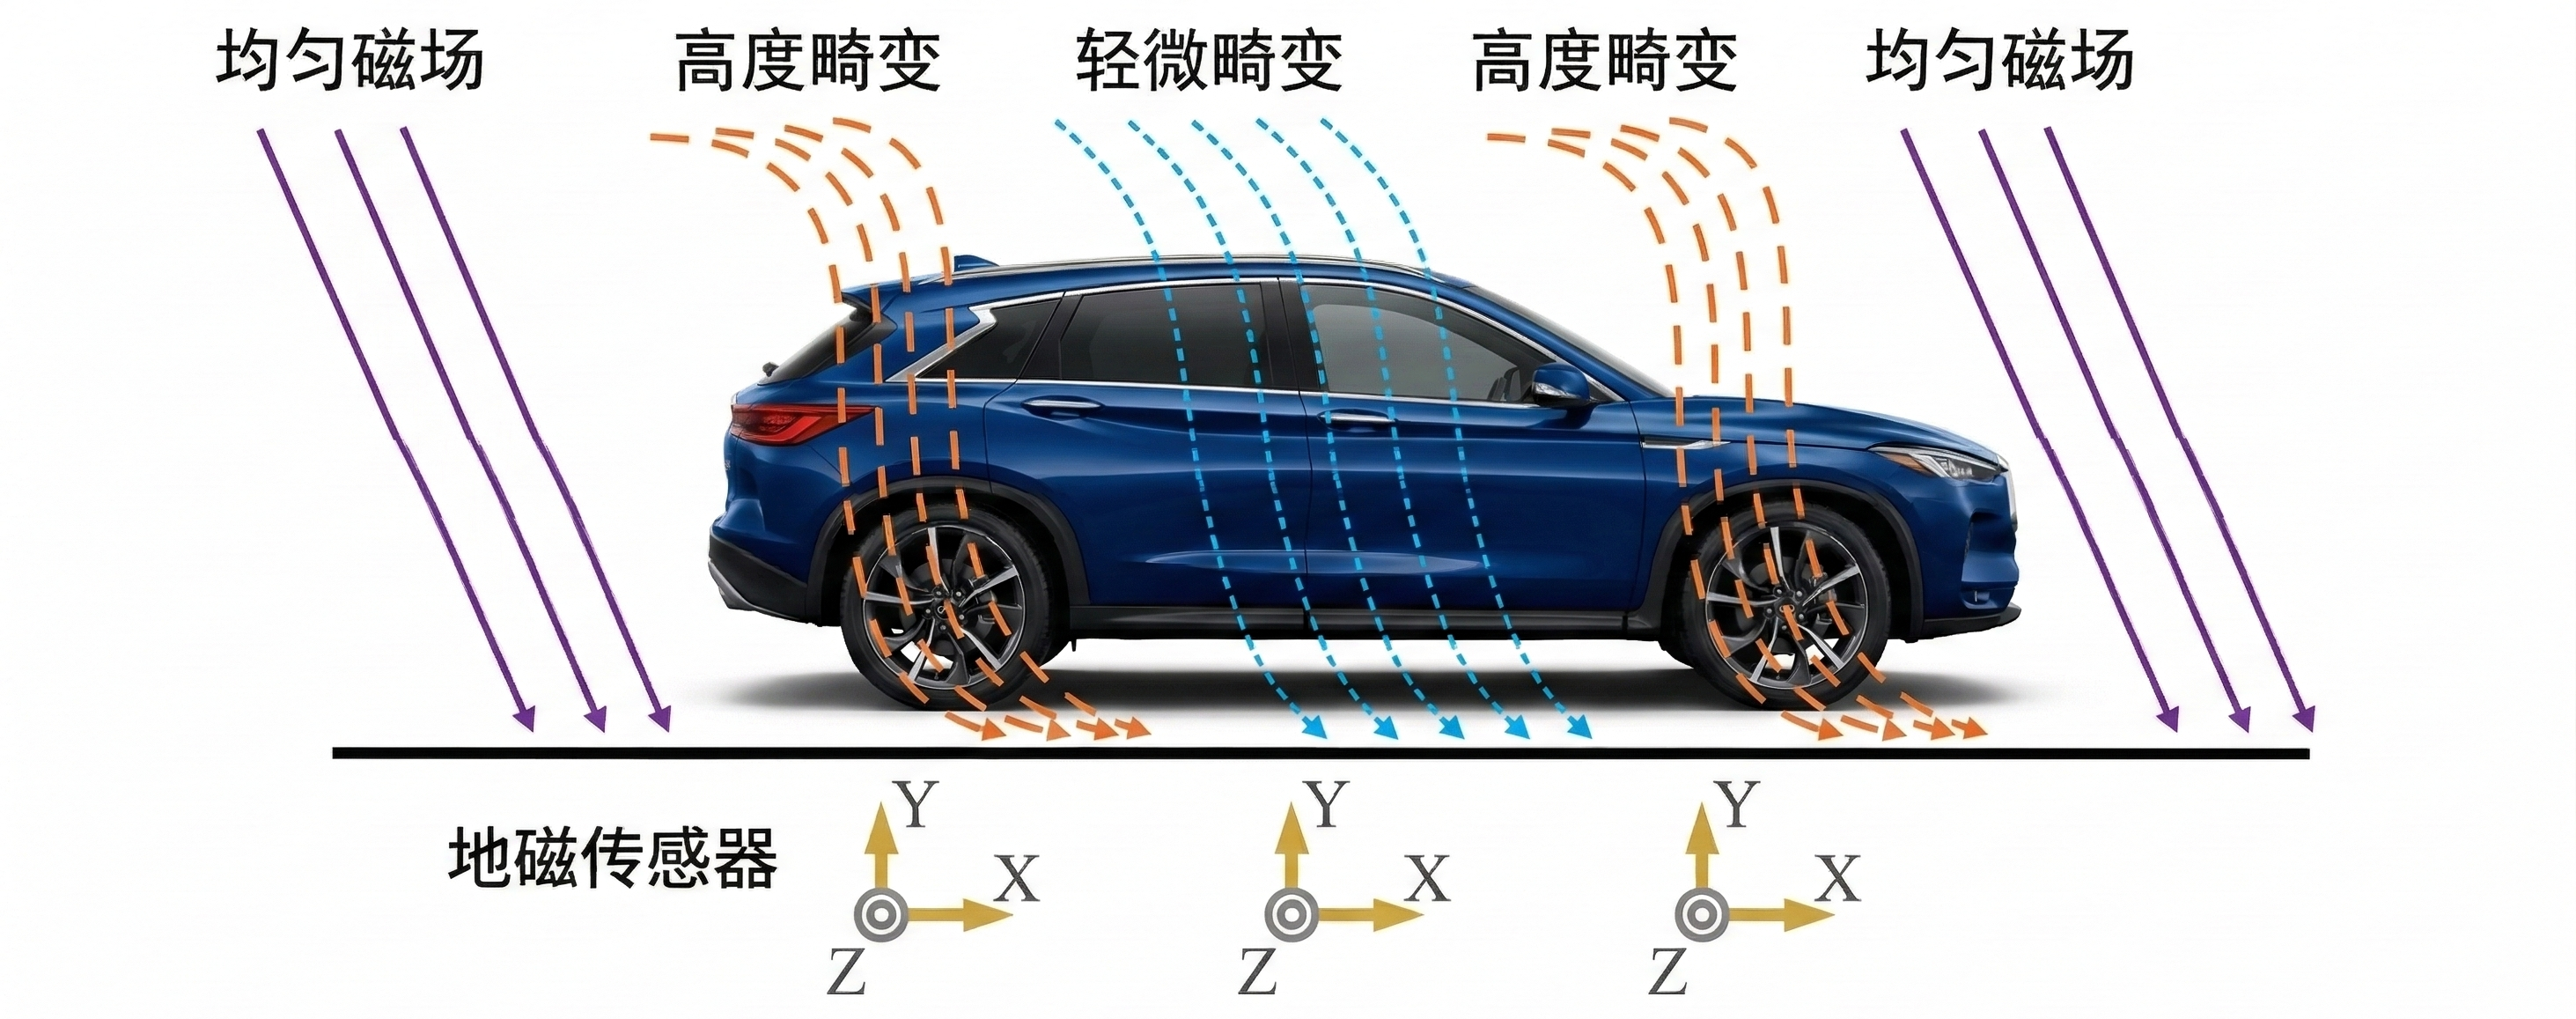
\includegraphics[width=0.85\textwidth]{images/chapter2/fig_2_1_mag_disturbance}
	\caption{车辆引起磁场扰动示意图}
	\label{fig:mag_disturbance}
\end{figure}

在上述机理基础上，车辆检测可进一步表述为事件化输出问题。通过估计无车基线并监测磁场偏移的变化，可确定车辆进入与离开对应的事件起止时刻，并由偏移幅值、持续时间及波形结构提取事件特征\cite{cheung2005traffic}。这类事件化描述不仅用于车辆存在性判定，也为后续速度估计、车辆分类以及跨传感器匹配提供基础输入，因此事件边界的稳定性与特征的一致性对后续目标跟踪具有直接影响。


\begin{figure}[htbp]
	\centering
	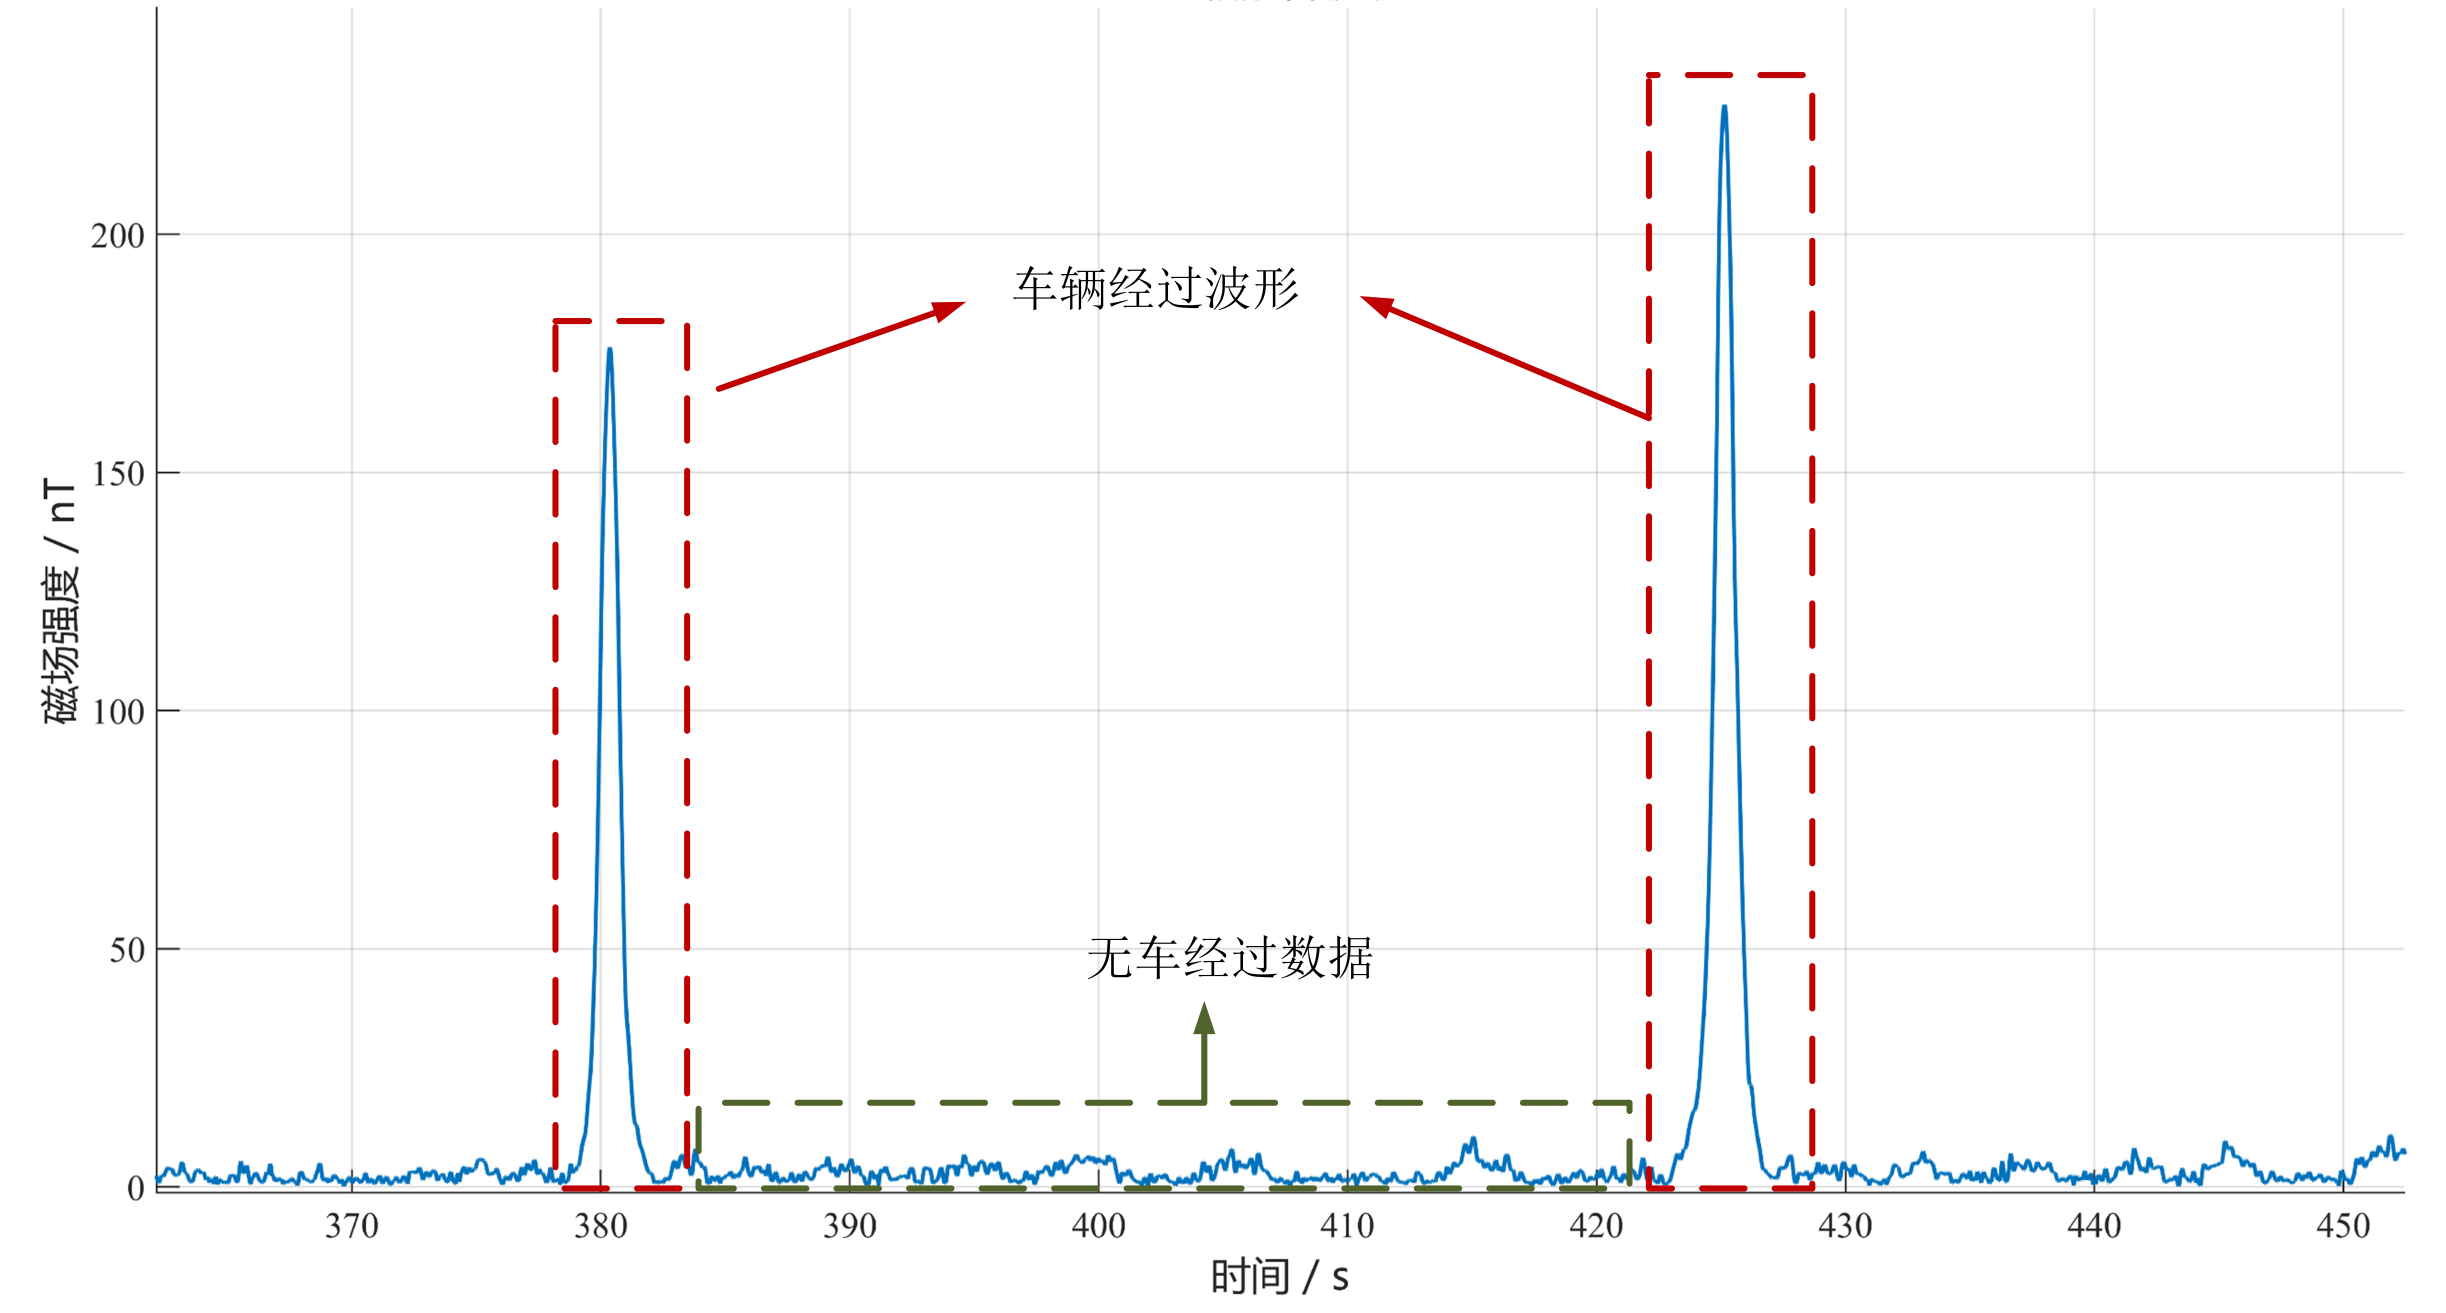
\includegraphics[width=0.85\textwidth]{images/chapter2/fig_2_2_mag_value}
	\caption{车辆经过时地磁传感器检测的磁场强度数据变化图}
	\label{fig:mag_value}
\end{figure}

同时需要注意，地磁扰动具有显著的空间衰减特性。车辆与传感器的横向距离增大时，扰动幅值会明显下降，信噪比随之降低，事件触发的可靠性与边界精度会受到影响，从而增加漏检风险。为获得更清晰的扰动响应与更稳定的事件特征，传感器通常布设在车道线附近，使车辆通过时具有更高的观测幅度与更可分的波形形态。



\subsection{地磁车辆检测算法}\label{sec:vehicle_detection}

地磁车辆检测的任务是在连续三轴磁场采样序列中识别由车辆通过引起的扰动区间，并在基线缓慢漂移与随机噪声叠加的条件下保持触发稳定。不同系统在采样频率、特征构造与上报字段上存在差异，但整体处理思路通常一致：先对原始观测进行平滑去噪并在线估计无车基线，再将三轴相对基线的偏移量压缩为标量检测统计量，最后通过判决逻辑确定车辆是否进入与离开，并据此生成检测记录。工程实现中，阈值判决与基于有限状态机的序列判决较为常见\cite{ding2004signalprocessing,sarcevic2022singlemagnetometer}。

为便于统一判决，设传感器在第 $k$ 个采样时刻的三轴磁场观测向量为
\[
\mathbf{B}(k)=
\begin{bmatrix}
	B_x(k)\\
	B_y(k)\\
	B_z(k)
\end{bmatrix},
\]
其中 $B_x(k)$、$B_y(k)$、$B_z(k)$ 分别表示 $x$、$y$、$z$ 三个轴向的磁场分量观测值；设 $\bar{\mathbf{B}}(k)$ 表示对应时刻的无车基线估计向量，通常由滑动平均、低通滤波或递推估计获得。基于此，可定义标量检测统计量：
\begin{equation}
	d(k)=\left\lVert \mathbf{B}(k)-\bar{\mathbf{B}}(k)\right\rVert_2
\end{equation}
其中，$d(k)$ 表示第 $k$ 个采样时刻的扰动强度，$\lVert\cdot\rVert_2$ 表示二范数。该统计量以幅值形式刻画三轴偏移的综合程度，能够将方向相关的波形差异转化为统一比较的幅值指标。由于 $d(k)$ 会随车型、车速、车辆相对传感器的通过位置以及姿态等因素产生幅值波动，同时基线也可能随温度或环境磁背景变化而缓慢漂移，因此检测阶段通常需要采用阈值自适应或引入序列一致性约束，以降低长期部署中阈值失配与抖动触发带来的稳定性下降\cite{sarcevic2022singlemagnetometer}。

在判决逻辑上，阈值判决通过比较 $d(k)$ 与阈值 $T$ 实现二值判定：当 $d(k)>T$ 时判为有车，否则判为无车，其中 $T$ 为判决阈值。该方法结构简单、计算代价低，适合在传感器端实时运行，但固定阈值对幅值变化与基线漂移较敏感。为提升不同工况下的可用性，可采用自适应阈值策略，根据近期噪声水平或统计量分布对 $T$ 进行在线更新，从而在车辆幅值变化或背景波动时维持较稳定的检出性能。

仅依赖逐点阈值比较时，$d(k)$ 在阈值附近的抖动可能引发重复触发或短脉冲误检。为抑制这类现象，常在阈值判决结果基础上引入状态机判决机制。有限状态机（Finite State Machine, FSM）是状态机判决的一种典型实现，其将检测过程划分为无车、进入确认、有车、离开确认等状态，并引入连续点数或最小持续时间约束：只有当进入条件持续满足一定长度时才确认车辆进入，同理只有离开条件持续满足一定长度时才确认车辆离开，从而提高对短时噪声与突发干扰的容忍度。在多车道环境下，还可结合多轴一致性、滞回阈值或车道约束等机制，降低相邻车道干扰引发的误检概率\cite{guilbert2016statemachine}。

当进入与离开时刻被稳定确定后，系统即可生成一条车辆检测记录。通常以进入时刻与离开时刻表征车辆在传感器有效探测区内的通过区间，并可进一步输出扰动峰值与持续时长等特征字段，为速度估计、占有率计算、车长推断以及跨点数据关联提供基础量测输入\cite{balid2018intelligent}。


\section{多地磁传感器部署模型及系统介绍}\label{sec:ch2_platform}

在完成地磁车辆检测并获得事件化输出后，多目标跟踪问题的输入不再是连续磁场波形，而是由多个地磁传感器节点在车辆通过时产生的离散量测序列。由于地磁传感器在空间上分布、节点时钟无法完全对齐且数据通过无线链路汇聚，量测在时间轴与空间轴上都呈现离散、异步和不完备特性。为使后续算法的推导具有统一的符号体系与明确的输入边界，本节从系统实现与数学建模两个层面给出多地磁车辆目标跟踪的基础描述。



\subsection{系统架构}
为将多地磁传感器采集到的车辆检测信息进一步用于目标跟踪，本文搭建了如图2.8所示的路侧感知与后台处理系统。系统的数据链路可以概括为三步：地磁传感器节点在路侧生成车辆检测数据，数据传输模块对多节点数据进行汇聚与回传，后台处理端在事件流输入条件下完成多目标跟踪与轨迹输出。系统由地磁传感器节点、数据传输模块和后台处理模块构成，各部分功能与数据流向如下。

\begin{figure}[htbp]
	\centering
	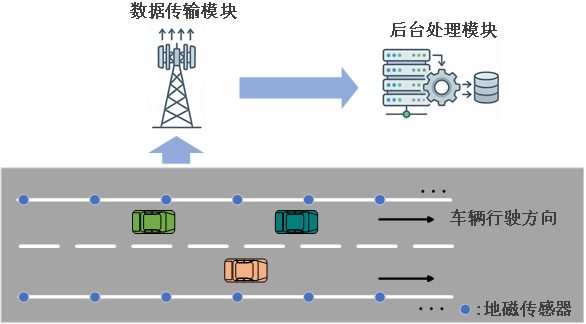
\includegraphics[width=0.65\textwidth]{images/chapter2/fig_2_5_system.png}
	\caption{地磁传感器车辆目标跟踪系统示意图}
	\label{fig:fig_2_5_system}
\end{figure}

首先，地磁传感器节点负责前端磁场连续采样与车辆通过检测。本系统采用一体化节点设计，将三轴地磁传感器 VCM5883、微控制单元 MCU、LoRa 通信模块以及太阳能供电与充电单元集成封装于同一设备中，实物如图2.9所示。VCM5883持续采集节点周围磁场变化并输出三轴磁场序列，MCU在端侧完成必要的预处理与判决，并运行状态机检测逻辑以识别车辆通过引起的磁扰动片段，从而生成车辆检测数据。检测数据以离散量测形式组织，通常包含触发时间戳、节点位置戳与反映磁扰动强度的特征量等字段。其中，触发时间戳与节点位置戳是后续时序组织与空间映射的基础信息，磁特征可作为补充线索用于提高复杂车流条件下的区分能力。节点生成检测记录后，经 LoRa 通信模块上报至路侧数据传输模块；太阳能供电与充电单元用于保障节点在无外接电源条件下的持续运行，提升长期部署的稳定性。需要指出的是，时间戳由节点本地时钟给出，不同节点之间可能存在静态或缓慢变化的时钟偏差，该偏差会表现为同一车辆在不同节点处量测时标的系统性错位，后续在量测建模与数据关联中需考虑其影响。

\begin{figure}[htbp]
	\centering
	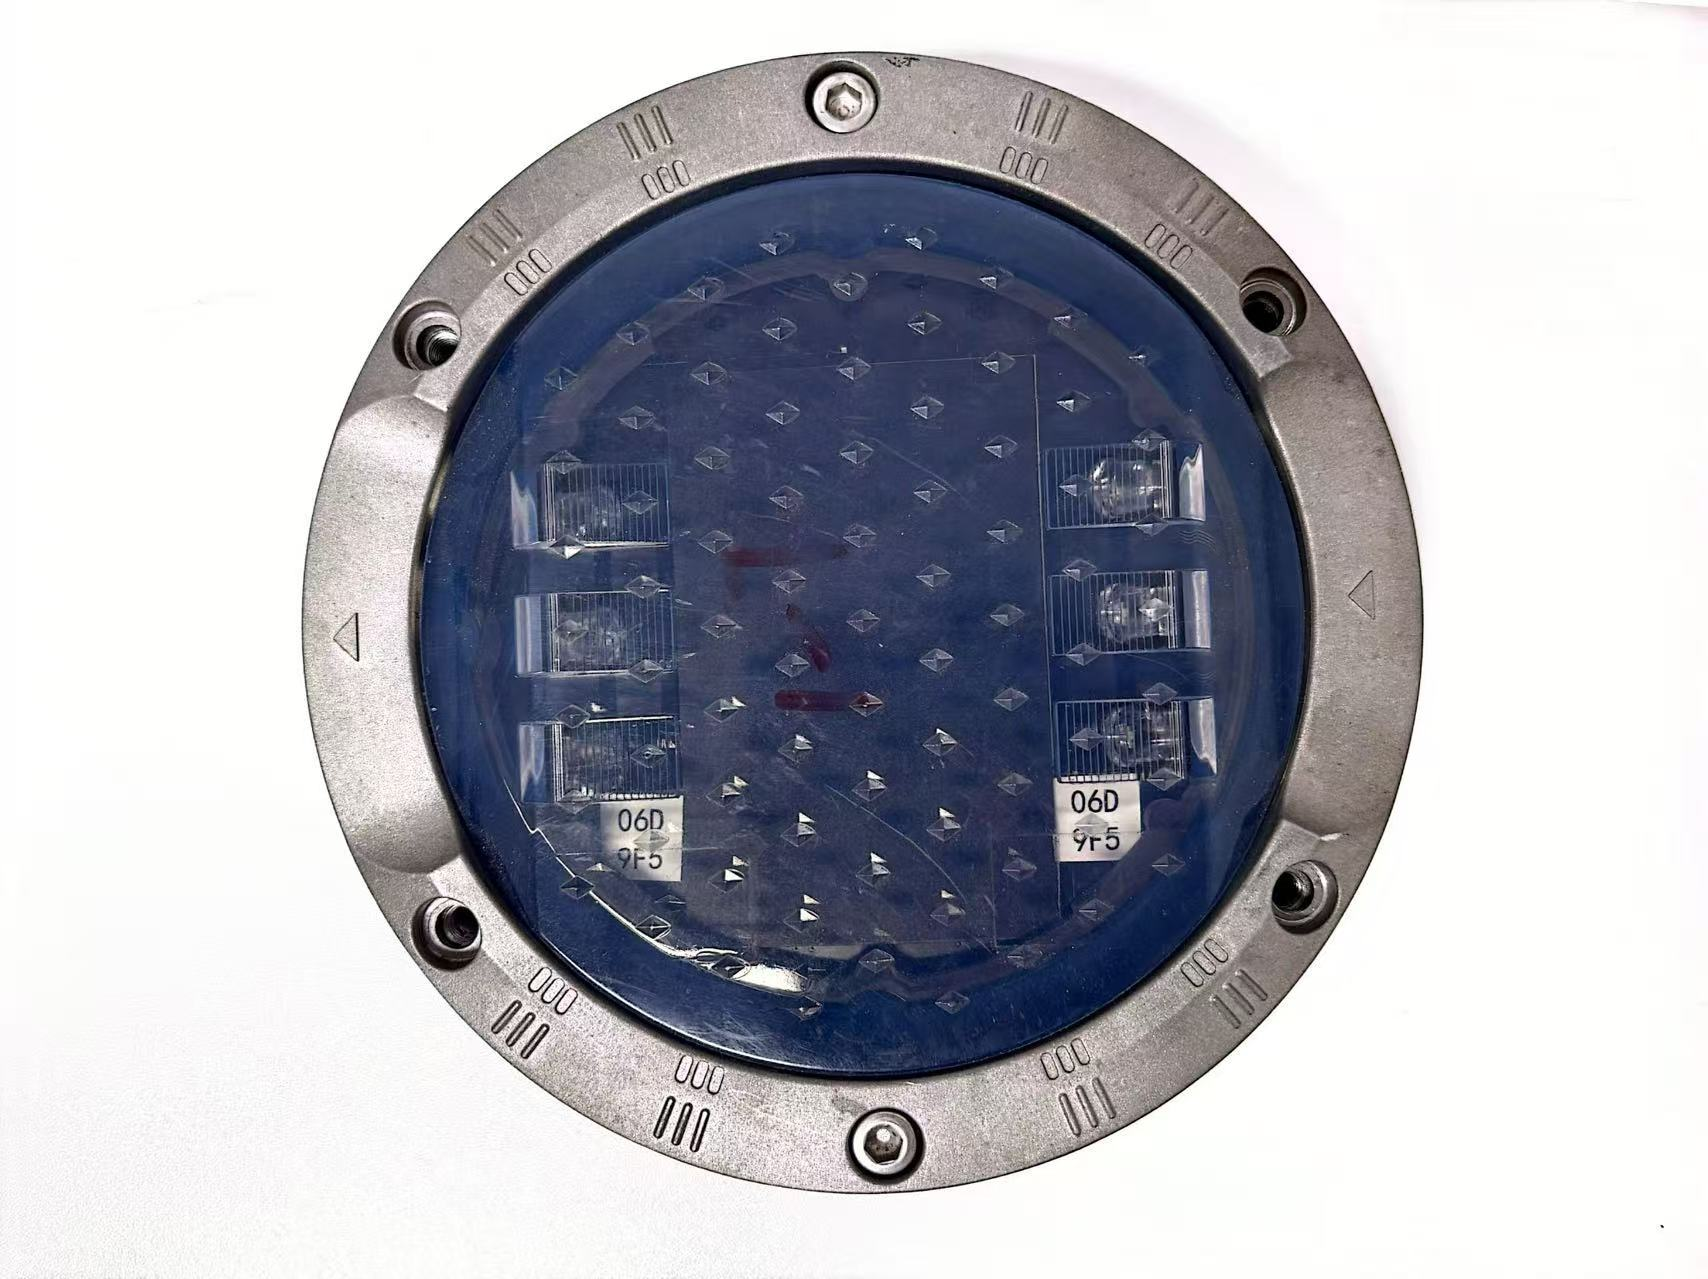
\includegraphics[width=0.45\textwidth]{images/chapter2/fig_2_4_geomagnetic_sensor}
	\caption{地磁传感器示意图}
	\label{fig_2_4_geomagnetic_sensor}
\end{figure}


其次，数据传输模块承担多节点数据汇聚与公网回传功能，其实物如图2.10所示。该模块为一体化物联网通信基站，具备 LoRa 近端通信与蜂窝网络远端回传两类能力。在近端通信侧，模块内置基于 LoRa 的私有协议，可与沿线部署的地磁传感器节点建立稳定无线连接，实现多节点检测记录的集中接入与可靠交互，有效通信距离可达约 5 km。在远端回传侧，通过插装物联网卡接入 4G 网络，模块与后台处理端建立通信链路，并按照预设周期将缓存的检测数据打包上传，从而实现多点事件数据的集中回传与后台统一接入。


\begin{figure}[htbp]
	\centering
	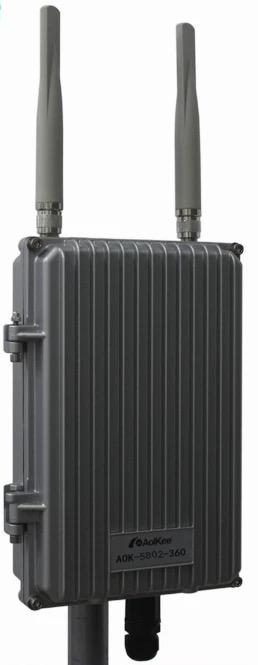
\includegraphics[width=0.15\textwidth]{images/chapter2/fig_2_1_base}
	\caption{物联网设备通信基站实物图}
	\label{fig_2_1_base}
\end{figure}

最后，后台处理模块承担数据流接入与在线跟踪计算两项核心任务，其作用是将数据传输模块回传的地磁检测信息转化为可持续更新的车辆跟踪结果。本文目前采用云服务器实现后台处理端，以便于集中管理、统一运行与后续扩展。在数据处理流程上，后台通过网络接口持续接收数据传输模块推送的事件数据流，完成数据解析与字段校验，并在多车并行条件下结合数据关联、状态估计与车道判别或实时聚类等处理，递推得到车辆在路段内的运动状态与行驶车道的时间序列估计，实现对车辆目标的连续跟踪。需要说明的是，检测数据流在后台侧按到达顺序进入处理链路，受无线链路时延与回传机制影响，部分观测可能出现随机延迟甚至迟到到达，导致观测到达顺序与实际触发时间顺序不一致，从而对关联与更新过程产生直接影响。这类时序不一致与缺测现象属于本文后续量测建模与算法设计需要显式考虑的非理想因素之一，相关方法将在后续章节中进一步展开。

\begin{figure}[htbp]
	\centering
	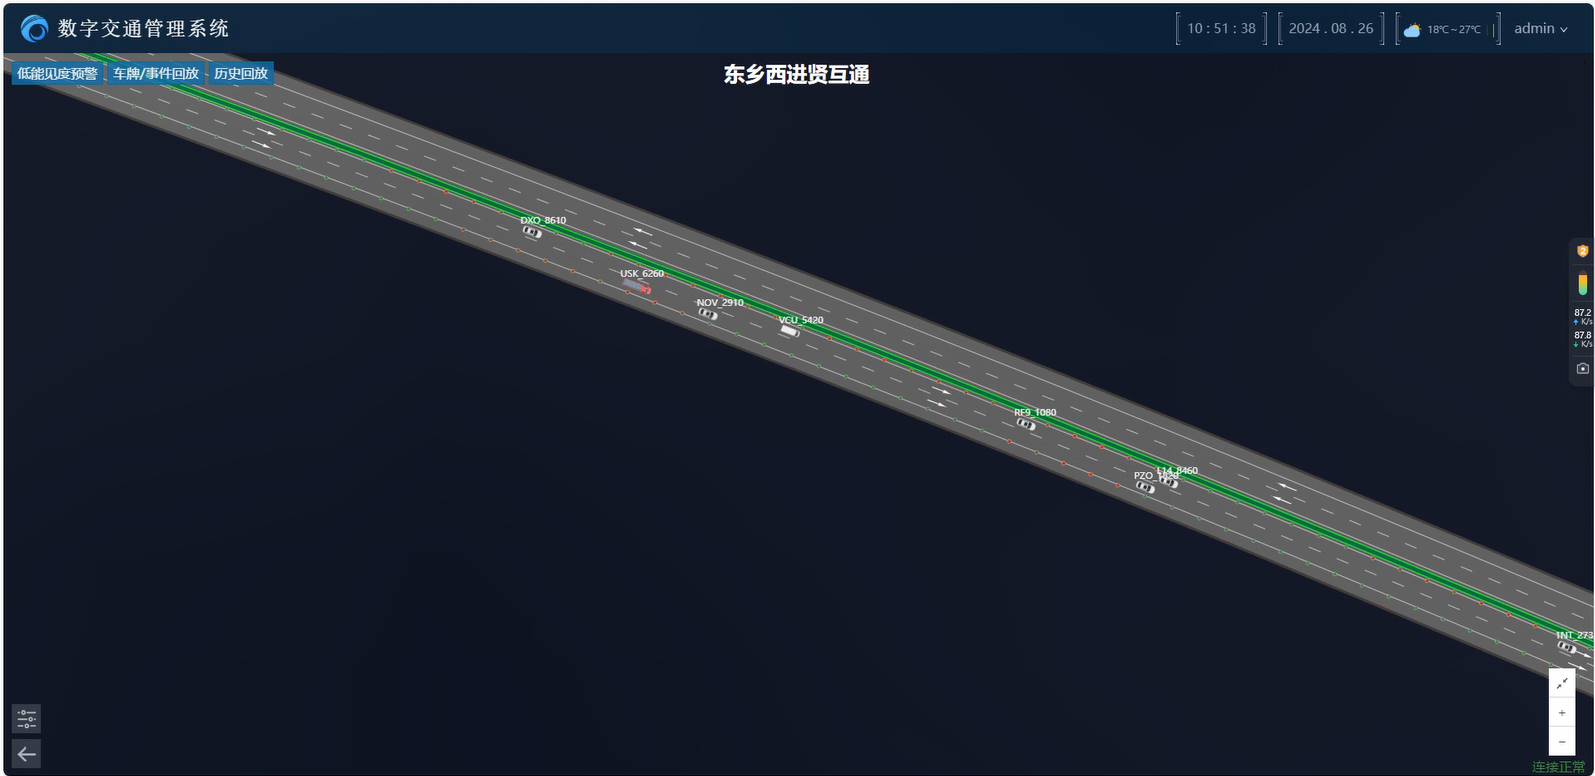
\includegraphics[width=0.85\textwidth]{images/chapter2/fig_2_7_platform}
	\caption{在线平台展示}
	\label{fig_2_7_platform}
\end{figure}



综上，图2.8所示系统贯通了数据流生成、无线汇聚回传与后台在线处理的完整流程，使多点地磁传感器检测记录能够以事件流形式进入目标跟踪算法。为进一步将检测记录形式化为可计算的时空量测，下一节将给出双车道场景下传感器空间布设与编号规则，并据此建立统一的量测表达。


\subsection{双车道多地磁传感器部署模型}\label{sec:ch2_summary}

图2.4给出了本文研究的单向双车道高速路段及其多地磁传感器布设方式。为获得可用于车辆目标跟踪的离散观测序列，本文沿车辆行驶方向以固定纵向间距布设多个观测位置；在每一个观测位置，分别在道路两侧边界车道线附近各布设一个地磁传感器节点，从而形成一组左右成对的观测点。图中实心圆点表示地磁传感器节点。车辆沿纵向行驶时将依次触发相邻观测位置处的节点并产生事件量测，这为后续的速度估计、数据关联与轨迹构建提供了基础输入。

\begin{figure}[htbp]
	\centering
	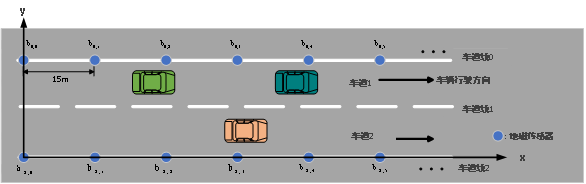
\includegraphics[width=0.85\textwidth]{images/chapter2/fig_2_8_road}
	\caption{单向双车道场景地磁传感器部署示意图}
	\label{fig_2_8_road}
\end{figure}

为便于后续建模与推导，建立道路坐标系：以车辆行驶方向为 $x$ 轴正方向，以横向跨车道方向为 $y$ 轴正方向，并取上游第一组传感器所在的纵向观测位置为坐标原点。本文仅考虑在两条边界车道线附近布设节点，并与后续车道线索引保持一致，将两条布设车道线编号为

\begin{equation}
	i \in \{0,2\}
	\tag{2-2}
\end{equation}

其中 $i=0$ 表示左侧边界车道线，$i=2$ 表示右侧边界车道线。沿行驶方向的观测位置按组编号记为

\begin{equation}
	k = 0,1,\ldots,K-1
	\tag{2-3}
\end{equation}

则位于车道线 $i$ 且属于第 $k$ 组观测位置的传感器记为 $b_{i,k}$。传感器节点的空间位置用二维坐标向量表示为

\begin{equation}
	\mathbf{s}_{i,k} =
	\begin{bmatrix}
		x_k \\
		y_i
	\end{bmatrix},
	\qquad
	i\in\{0,2\},\; k=0,1,\ldots,K-1
	\tag{2-4}
\end{equation}

其中 $x_k$ 为第 $k$ 个纵向观测位置的坐标，$y_i$ 为对应边界车道线的横向坐标。本文采用对称布设方式，即同一组中的 $b_{0,k}$ 与 $b_{2,k}$ 位于同一纵向观测位置（具有相同的 $x_k$），二者仅在横向位置 $y$ 上不同。相邻两组观测位置的纵向间距记为 $L_a$，则

\begin{equation}
	x_k = x_0 + kL_a,
	\qquad k=0,1,\ldots,K-1
	\tag{2-5}
\end{equation}

其中 $x_0$ 为第一组观测位置的纵向坐标，后续推导中通常取 $x_0=0$ 以简化表达。

需要指出的是，对称布设在工程实现与空间标定上更为直接，但在双车道并行行驶与换道条件下也会增强数据关联的歧义性：一方面，同一纵向观测位置同时存在左右两个观测点，多车并行时不同车辆的事件在时间轴上更易邻近甚至交叠；另一方面，车辆横向位置变化可能导致左右节点的触发强度与触发时刻出现偏移，从而使事件序列的对应关系更难仅凭时空邻近判定。基于上述部署模型，下一节将给出事件量测的统一表示，并结合理想与非理想事件流示例说明后续跟踪需要面对的主要不确定性来源。

\subsection{双车道多地磁传感器测量模型}

地磁传感器节点检测到车辆通过后，会向后台上报一条检测记录。将后台按到达顺序接收的第 $j$ 条记录记为量测向量 $\mathbf z_j$，结合本文系统的上报格式，量测可定义为
\begin{equation}
	\mathbf z_j=
	\begin{bmatrix}
		t_j &
		id_j &
		x_{id_j} &
		y_{id_j} &
		\ell_{id_j} &
		Mpeak_j
	\end{bmatrix}^{\mathrm T},
	\label{eq:ch3_zj_v2}
\end{equation}
其中，$t_j$ 为触发时间戳，$id_j$ 为地磁传感器设备编号，$x_{id_j}$ 和 $y_{id_j}$ 分别为该设备在道路坐标系下的纵向和横向安装坐标，$\ell_{id_j}$ 为该设备所属边界车道线编号，$Mpeak_j$ 为该次触发片段上报的地磁峰值。式~\eqref{eq:ch3_zj_v2} 描述了车辆在时刻 $t_j$ 于观测点 $(x_{id_j},y_{id_j})$ 附近形成的一次离散量测。

\subsubsection{ 理想检测数据流形态}


图2.5(a)给出了理想情况下检测数据流的典型形态。图中以时间戳为横轴、设备编号为纵轴，每一个散点对应一条检测记录。

\begin{figure}[htbp]
	\centering
	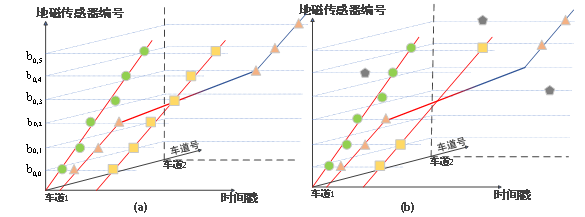
\includegraphics[width=0.85\textwidth]{images/chapter2/fig_2_9_data}
	\caption{地磁传感器数据理想情况与非理想情况}
	\label{fig_2_9_data}
\end{figure}

如图所示，同一车辆沿路段向下游行驶时，其检测点会随纵向布设顺序逐步出现在更下游的观测位置上，在 $\text{Time--SensorID}$ 平面内呈现近似单调上升的轨迹结构。当车速变化不剧烈时，同一车辆在相邻两个纵向观测位置处的触发时间差满足近似关系

\begin{equation}
	t_{k+1}-t_k \approx \frac{L_a}{v}
	\tag{2-7}
\end{equation}

其中 $L_a$ 为相邻观测位置的纵向间距，$v$ 为车辆纵向速度。由此可见，理想条件下检测点在时间轴与空间轴上具有较强的连续性，这为后续门控与数据关联提供了几何先验。此外，车辆在车道内保持直行时，其检测点通常持续出现在同一侧传感器序列上，如图2.5(a)中绿色圆形、黄色方形所连接轨迹所示；而发生换道时，检测点会在两侧传感器序列之间出现切换或过渡，如图2.5(a)中橙色三角所连接跨车道轨迹所示。

\subsubsection{非理想检测数据流形态}


真实道路环境下，检测数据流通常表现为图2.5(b)所示的非理想形态，与图2.5(a)相比主要差异可归纳为以下三类。

首先是漏检导致的量测缺失。部分观测位置未产生检测点，既可能是单次缺失，也可能在若干相邻观测位置上连续缺失，从而使同一车辆的检测点出现明显空档并导致轨迹结构断裂，如橙色三角所连轨迹在变道过程中丢失关键数据点 $b_{2,3}$，而黄色方形所连接轨迹连续丢失 $b_{1,3}$、$b_{1,4}$、$b_{1,5}$ 三个数据点。这会直接削弱由时间差推得的速度约束，并增大关联不确定性。

其次是虚警导致的杂波量测。相邻车道干扰、环境噪声或异常电磁扰动可能产生与真实车辆无关的检测点，其分布通常较为离散且缺乏连续结构。图2.5(b)中的灰色五边形散点即为典型杂波样本，它们会扩大候选关联集合，增加误关联风险，尤其在车流密集时更为突出。

最后是时间戳误差与迟到到达。节点时钟偏差与链路延迟会导致时间戳偏移或观测迟到，从而使同一车辆的检测点在时间轴上出现错位或局部乱序。

根据图2.7所示的测量模型，本文研究的多地磁传感器多车辆目标跟踪算法的目标是利用车辆经过多个地磁传感器时所产生的检测时间以及车辆磁场强度等测量值，在存在传感器时间误差、漏检和虚警等条件下，实现车辆与地磁传感器测量数据之间的可靠关联，并对车辆运动状态以及车辆行驶车道等信息进行准确估计。同时进一步探讨在系统长期运行导致连续多次漏检情况下的鲁棒车辆跟踪方法。


\section{卡尔曼滤波算法}

由于杂波干扰以及传感器本身存在的测量不准确性，传感器提供的测量值与目标的真实值之间通常存在偏差，因此需要采用滤波算法对目标状态进行估计，减小不确定性带来的影响。卡尔曼滤波是多目标领域中重要的跟踪滤波算法，其主要用于线性动态系统的目标跟踪。卡尔曼滤波的基本流程如图~2.11 所示，通过建立目标的运动模型，卡尔曼滤波将目标运动状态的预测值与传感器测量值进行加权融合，得到对目标运动状态的估计。卡尔曼滤波估计的优点是其只需要保留前一时刻的估计状态，运算的复杂性不高，同时在线性系统中具有良好的跟踪性能。

\subsection{卡尔曼滤波算法的过程}

在卡尔曼滤波过程中，首先需要建立目标运动模型与观测模型，目标运动模型与观测模型的离散时间状态方程分别表示为：
\begin{equation}
	x(k)=F(k-1)x(k-1)+W(k-1)
	\tag{2-2}
\end{equation}

\begin{equation}
	z(k)=H(k)x(k)+V(k)
	\tag{2-3}
\end{equation}

其中，$x(k)$ 表示 $k$ 时刻目标运动状态，$F(k-1)$ 为目标的状态转移矩阵。$z(k)$ 表示 $k$ 时刻的测量，$H(k)$ 为系统的观测矩阵。$W(k-1)$ 为系统的过程噪声，$V(k)$ 为系统测量噪声，假设过程噪声与测量噪声之间相互独立，且均服从均值为零的高斯分布，则有以下约束条件成立：
\begin{equation}
	E\!\left(W(k)W^{T}(j)\right)=Q(k)\delta_{kj}
	\tag{2-4}
\end{equation}

\begin{equation}
	E\!\left(V(k)V^{T}(j)\right)=R(k)\delta_{kj}
	\tag{2-5}
\end{equation}

\begin{equation}
	E\!\left(W(k)V^{T}(k)\right)=0
	\tag{2-6}
\end{equation}

其中，$Q(k)$ 为 $k$ 时刻系统过程噪声协方差矩阵，$R(k)$ 为 $k$ 时刻系统测量噪声协方差矩阵。$\delta_{kj}$ 为 Delta 函数，有：
\begin{equation}
	\delta_{kj}=
	\begin{cases}
		1, & k=j,\\
		0, & k\neq j.
	\end{cases}
	\tag{2-7}
\end{equation}

卡尔曼滤波器的估计过程分为状态预测和测量更新两个步骤。其中状态预测是通过当前目标的状态估计预测下一时刻的目标状态，公式为：
\begin{equation}
	\hat{x}(k|k-1)=F(k-1)\hat{x}(k-1|k-1)
	\tag{2-8}
\end{equation}

\begin{equation}
	P(k|k-1)=F(k-1)P(k-1|k-1)F^{T}(k-1)+Q(k-1)
	\tag{2-9}
\end{equation}

其中，$\hat{x}(k|k-1)$ 代表由 $k-1$ 时刻的信息对 $k$ 时刻目标的状态预测，$P(k|k-1)$ 代表状态预测的协方差矩阵。

测量更新的作用是将测量信息与状态预测进行融合，以获得更优的后验估计。在测量更新过程中，新息向量的计算公式为：
\begin{equation}
	\eta(k)=z(k)-H(k)\hat{x}(k|k-1)
	\tag{2-10}
\end{equation}

新息的协方差矩阵为：
\begin{equation}
	S(k)=H(k)P(k|k-1)H^{T}(k)+R(k)
	\tag{2-11}
\end{equation}

卡尔曼滤波增益为：
\begin{equation}
	K(k)=P(k|k-1)H^{T}(k)S^{-1}(k)
	\tag{2-12}
\end{equation}

最终滤波结果如下：
\begin{equation}
	\hat{x}(k|k)=\hat{x}(k|k-1)+K(k)\eta(k)
	\tag{2-13}
\end{equation}

\begin{equation}
	P(k|k)=P(k|k-1)-K(k)H(k)P(k|k-1)
	\tag{2-14}
\end{equation}

其中，$\hat{x}(k|k)$ 即为卡尔曼滤波融合目标预测值与测量值得到的在 $k$ 时刻关于目标运动状态的后验估计，$P(k|k)$ 为 $k$ 时刻对应的状态估计的协方差矩阵。

卡尔曼滤波器的性能很大程度上受到目标运动模型选择的影响。下面介绍卡尔曼滤波器中常见的运动模型与过程噪声的选取。

\subsection{目标运动模型}

卡尔曼滤波以及大多数跟踪器都是基于目标运动模型进行的，目标运动模型描述了目标的运动状态随时间的变化情况，选择合适的目标运动模型有助于目标状态的准确估计。根据目标的运动学特征，常见的目标运动模型包括常速度（Constant Velocity，CV）模型、常加速度（Constant Acceleration，CA）模型以及匀速转弯（Constant Turn，CT）模型等。

\subsubsection{CV 模型}

常速度模型假设目标进行匀速直线运动，即目标的加速度在理想情况下应为零，但是由于实际应用中干扰的存在，目标的加速度不可能严格为零，因此 CV 模型将加速度认为是均值为零的高斯白噪声来描述加速度带来的干扰。

状态转移矩阵表示为：
\begin{equation}
	F(k)=
	\begin{bmatrix}
		1 & T_k\\
		0 & 1
	\end{bmatrix}
	\tag{2-15}
\end{equation}

噪声增益向量表示为：
\begin{equation}
	\Gamma(k)=
	\begin{bmatrix}
		\dfrac{1}{2}T_k^2\\
		T_k
	\end{bmatrix}
	\tag{2-16}
\end{equation}

过程噪声的协方差矩阵计算公式为：
\begin{equation}
	Q(k)=\Gamma(k)\sigma_w^2\Gamma^{T}(k)=
	\begin{bmatrix}
		\dfrac{1}{4}T_k^4 & \dfrac{1}{2}T_k^3\\[6pt]
		\dfrac{1}{2}T_k^3 & T_k^2
	\end{bmatrix}\sigma_w^2
	\tag{2-17}
\end{equation}

其中，$T_k$ 为 $k-1$ 时刻与 $k$ 时刻之间的时间间隔，$\sigma_w$ 表示过程噪声的标准差。在文献[19]中提到 CV 模型中 $\sigma_w$ 的取值与目标的最大加速度 $a_M$ 的数量级有关，在实际使用中，其取值范围可以考虑为
\[
0.5a_M \leq \sigma_w \leq a_M.
\]

\subsubsection{CA 模型}

常加速度模型假设过程噪声 $W(k)$ 为加速度的增量，这种增量是均值为零的白噪声序列，也就是说，加速度为离散时间维纳过程。以目标在一维空间内运动为例，状态向量为目标的位置、速度和加速度。

状态转移矩阵表示为：
\begin{equation}
	F(k)=
	\begin{bmatrix}
		1 & T_k & \dfrac{T_k^2}{2}\\
		0 & 1   & T_k\\
		0 & 0   & 1
	\end{bmatrix}
	\tag{2-18}
\end{equation}

噪声增益向量表示为：
\begin{equation}
	\Gamma(k)=
	\begin{bmatrix}
		\dfrac{T_k^2}{2}\\
		T_k\\
		1
	\end{bmatrix}
	\tag{2-19}
\end{equation}

过程噪声的协方差矩阵计算公式为：
\begin{equation}
	Q(k)=\Gamma(k)\sigma_q^2\Gamma^{T}(k)=
	\begin{bmatrix}
		\dfrac{1}{4}T_k^4 & \dfrac{1}{2}T_k^3 & \dfrac{1}{2}T_k^2\\[6pt]
		\dfrac{1}{2}T_k^3 & T_k^2 & T_k\\[6pt]
		\dfrac{1}{2}T_k^2 & T_k & 1
	\end{bmatrix}\sigma_q^2
	\tag{2-20}
\end{equation}

在文献[19]有关 CA 模型的讨论中，$\sigma_q$ 的取值与在两次更新时刻时间内目标的最大加速度增量 $\Delta a_M$ 有关，在实际使用中其取值范围可以考虑为
\[
0.5\Delta a_M \leq \sigma_q \leq \Delta a_M.
\]

\subsubsection{CT 模型}

CT 模型主要用来描述目标运动过程中的转弯运动，其假设目标在转弯过程中以匀角速度运动，通过设置转弯角速度对目标的转弯运动中的状态进行估计。令 $\omega$ 代表目标的转弯角速度，在二维坐标系中，目标的状态向量为
\[
x(k+1)=[x,\ v_x,\ y,\ v_y]^T,
\]
则 CT 模型的离散状态方程表示为：
\begin{equation}
	x(k+1)=
	\begin{bmatrix}
		1 & \dfrac{\sin \omega T}{\omega} & 0 & -\dfrac{1-\cos \omega T}{\omega}\\[8pt]
		0 & \cos \omega T & 0 & -\sin \omega T\\[6pt]
		0 & \dfrac{1-\cos \omega T}{\omega} & 1 & \dfrac{\sin \omega T}{\omega}\\[8pt]
		0 & \sin \omega T & 0 & \cos \omega T
	\end{bmatrix}
	x(k)
	+
	\begin{bmatrix}
		\dfrac{T^2}{2}\\
		T\\
		\dfrac{T^2}{2}\\
		T
	\end{bmatrix}
	w(k)
	\tag{2-21}
\end{equation}

目标转弯角速度 $\omega$ 控制了目标的转弯速度以及转弯方向，通过引入 $\omega$，使得 CT 模型可以用来描述正在进行转弯的机动目标。



\section{数据关联算法}\label{sec:orm}
多目标跟踪中，滤波器负责在给定量测来源的前提下递推估计目标状态，而数据关联负责在每次更新时刻确定量测与目标航迹之间的对应关系。由于实际环境中存在杂波、漏检以及目标数目随时间变化等因素，量测的来源往往无法直接判定，导致关联决策成为影响跟踪精度与身份稳定性的关键环节。工程上常用的数据关联流程通常包括三步。首先根据各航迹的预测信息在量测空间构造跟踪波门，剔除显然不可能来自该航迹的量测。其次在波门内计算量测与航迹之间的一致性度量，例如欧氏距离、马氏距离或基于似然的代价。最后在互斥约束下完成量测分配并进行航迹更新，同时对未分配量测与未更新航迹按管理规则处理。后续章节将在该通用框架下，引入软关联与多扫描一致性推断，以降低密集场景下的误关联与身份切换。

为避免与第2.3节传感器沿纵向的索引符号混淆，下文以$t_k$表示第$k$次更新对应的时间戳，$k=1,2,\ldots$仅表示更新序号。记目标状态在$t_k$处的离散表示为$\mathbf{x}_k \triangleq \mathbf{x}(t_k)$。在更新时刻$t_k$，滤波器根据上一时刻$t_{k-1}$的后验估计对各条活动航迹进行预测，得到预测航迹集合

\begin{equation}
	\mathcal{T}_{k|k-1}=\left\{\mathcal{T}^{(i)}_{k|k-1}\right\}_{i=1}^{N_k},
\end{equation}

其中$N_k$为参与本次更新的预测航迹条数，$\mathcal{T}^{(i)}_{k|k-1}$表示第$i$条预测航迹。通常用$\hat{\mathbf{x}}^{(i)}_{k|k-1}$与$\mathbf{P}^{(i)}_{k|k-1}$分别表示其预测状态均值与预测协方差。同一更新时刻用于更新的量测构成量测集合

\begin{equation}
	\mathcal{Z}_k=\left\{\mathbf{z}^{(j)}_k\right\}_{j=1}^{M_k},
\end{equation}

其中$M_k$为量测数，$\mathbf{z}^{(j)}_k$为第$j$个量测。一般情况下，$\mathcal{Z}_k$包含真实目标量测与杂波量测，且真实目标可能发生漏检。

为描述航迹与量测之间的一对一指派关系，引入关联变量

\begin{equation}
	\theta_k^{(i)}\in\left\{0,1,2,\ldots,M_k\right\},
\end{equation}

其中$\theta_k^{(i)}=j$表示第$i$条航迹与量测$\mathbf{z}^{(j)}_k$建立关联，$\theta_k^{(i)}=0$表示第$i$条航迹在$t_k$未获得有效量测更新。等价地，可用二值指派矩阵$\mathbf{A}_k=[a_{i,j}]$表示指派结果，其元素定义为

\begin{equation}
	a_{i,j}=
	\begin{cases}
		1, & \text{量测 }\mathbf{z}^{(j)}_k \text{分配给航迹 } i,\\
		0, & \text{否则}.
	\end{cases}
\end{equation}

在经典的一对一关联假设下，指派矩阵需满足互斥约束

\begin{equation}
	\sum_{j=1}^{M_k} a_{i,j}\le 1,\qquad i=1,\ldots,N_k,
\end{equation}
\begin{equation}
	\sum_{i=1}^{N_k} a_{i,j}\le 1,\qquad j=1,\ldots,M_k.
\end{equation}

其中第一式表示每条航迹至多选择一个量测，第二式表示每个量测至多分配给一条航迹。未被分配的量测通常视为杂波，未获得量测的航迹对应漏检或暂不更新情形。

\subsection{跟踪波门}

跟踪波门用于在进入关联求解之前剔除明显不可能的轨迹与量测候选对，从而减少候选规模、降低误关联风险，并提高后续关联计算的效率与稳定性。其基本思想是依据目标轨迹的预测量测及其不确定性，在量测空间内构造一个有限候选区域，仅保留落入该区域的量测参与后续关联。工程中常见的波门形式包括矩形波门、扇形波门和椭球波门，其中矩形波门实现简单，扇形波门适用于方向约束较强的场景，而椭球波门能够同时反映预测误差与量测噪声的统计特性，因此在目标跟踪中应用最为广泛。结合本文后续关联建模过程，采用椭球波门进行候选量测筛选。

设轨迹 $i$ 在时刻 $t_k$ 的预测量测为 $\hat{\mathbf{z}}^{(i)}_{k|k-1}$，第 $j$ 个量测为 $\mathbf{z}^{(j)}_k$，则对应的创新向量可写为
\begin{equation}
	\boldsymbol{\nu}^{(i,j)}_k
	=
	\mathbf{z}^{(j)}_k-\hat{\mathbf{z}}^{(i)}_{k|k-1}.
\end{equation}
在卡尔曼滤波框架下，其创新协方差为
\begin{equation}
	\mathbf{S}^{(i)}_k
	=
	\mathbf{H}_k \mathbf{P}^{(i)}_{k|k-1}\mathbf{H}_k^\top+\mathbf{R}_k.
\end{equation}
进一步定义平方马氏距离为
\begin{equation}
	d_k^2(i,j)
	=
	\left(\boldsymbol{\nu}^{(i,j)}_k\right)^\top
	\left(\mathbf{S}^{(i)}_k\right)^{-1}
	\boldsymbol{\nu}^{(i,j)}_k .
\end{equation}
给定波门概率 $P_G$，取门限 $\gamma=\chi_m^2(P_G)$，则椭球波门可表示为
\begin{equation}
	\mathcal{G}^{(i)}_k
	=
	\left\{
	j \,\big|\, d_k^2(i,j)\le \gamma
	\right\}.
\end{equation}
由此，仅保留满足门限约束的候选量测进入后续关联求解。该波门形式能够根据预测协方差自适应调节候选区域大小，在候选筛选效率与真实量测保留能力之间取得较好的平衡。

\subsection{硬关联方法与匈牙利算法}

硬关联方法在每个更新时刻输出确定的一对一指派结果。设 $c_{i,j}$ 为将量测 $j$ 分配给航迹 $i$ 的代价。令 $\mathbf{A}_k=[a_{i,j}]$ 为指派矩阵，则单时刻一对一指派可表述为线性指派问题
\begin{align}
	\min_{\mathbf{A}_k}\quad 
	& \sum_{i=1}^{N_k}\sum_{j=1}^{M_k} c_{i,j}\,a_{i,j} \\
	\text{s.t.}\quad
	& a_{i,j}\in\{0,1\}, \\
	& \sum_{j=1}^{M_k} a_{i,j}\le 1, \\
	& \sum_{i=1}^{N_k} a_{i,j}\le 1 .
\end{align}

当候选对 $(i,j)$ 落在跟踪波门外时，通常将 $c_{i,j}$ 置为较大值以避免不合理匹配。匈牙利算法是求解线性指派问题的经典方法，能够在多项式时间内得到全局最优的一对一指派解，因此常作为在线跟踪系统的单时刻硬关联基线。

\subsection{概率数据关联方法}

概率数据关联方法在波门内存在多个候选量测且难以可靠做出硬决策时，引入关联概率对候选量测进行加权更新，从而降低误关联对状态估计的破坏。PDA用于单目标情形，JPDA扩展到多目标并显式考虑互斥约束。二者均以关联概率为核心，通过对候选量测进行加权实现状态更新。


\subsubsection{PDA的基本形式}

对航迹 $i$，门内量测 $j\in\mathcal{G}^{(i)}_k$ 的量测似然可写为
\begin{equation}
	L_{i,j}
	=
	\mathcal{N}\!\left(
	\mathbf{z}^{(j)}_k;
	\hat{\mathbf{z}}^{(i)}_{k|k-1},
	\mathbf{S}^{(i)}_k
	\right),
\end{equation}
其中 $\mathcal{N}(\mathbf{z};\boldsymbol{\mu},\mathbf{\Sigma})$ 表示均值为 $\boldsymbol{\mu}$、协方差为 $\mathbf{\Sigma}$ 的高斯概率密度。考虑漏检与杂波，引入检测概率 $P_D$ 以及杂波空间密度 $\lambda$。若以 $V_k^{(i)}$ 表示航迹 $i$ 在 $t_k$ 的波门体积，则门内杂波的期望数量为 $\lambda V_k^{(i)}$。常用的归一化关联概率可写为
\begin{equation}
	\beta_{i,j}
	=
	\frac{P_D\,L_{i,j}}
	{\lambda V_k^{(i)} + P_D\sum\limits_{\ell\in\mathcal{G}^{(i)}_k}L_{i,\ell}},
\end{equation}
并定义漏检概率质量为
\begin{equation}
	\beta_{i,0}
	=
	1-\sum_{j\in\mathcal{G}^{(i)}_k}\beta_{i,j}.
\end{equation}
其中，$\beta_{i,j}$ 表示量测 $j$ 来自航迹 $i$ 的关联概率，$\beta_{i,0}$ 表示航迹 $i$ 在 $t_k$ 未获得有效量测更新的概率。

在线性高斯条件下，航迹 $i$ 对应的卡尔曼增益为
\begin{equation}
	\mathbf{K}^{(i)}_k
	=
	\mathbf{P}^{(i)}_{k|k-1}\mathbf{H}_k^\top
	\left(\mathbf{S}^{(i)}_k\right)^{-1}.
\end{equation}
定义加权创新为
\begin{equation}
	\bar{\boldsymbol{\nu}}^{(i)}_k
	=
	\sum_{j\in\mathcal{G}^{(i)}_k}\beta_{i,j}\,\boldsymbol{\nu}^{(i,j)}_k,
\end{equation}
则均值更新可写为
\begin{equation}
	\hat{\mathbf{x}}^{(i)}_{k|k}
	=
	\hat{\mathbf{x}}^{(i)}_{k|k-1}
	+
	\mathbf{K}^{(i)}_k\,\bar{\boldsymbol{\nu}}^{(i)}_k.
\end{equation}
协方差更新除常规项外，还需考虑关联不确定性引入的扩张项，常用表达为
\begin{equation}
	\mathbf{P}^{(i)}_{k|k}
	=
	\mathbf{P}^{(i)}_{k|k-1}
	-
	\left(1-\beta_{i,0}\right)\mathbf{K}^{(i)}_k\mathbf{S}^{(i)}_k\left(\mathbf{K}^{(i)}_k\right)^\top
	+
	\mathbf{K}^{(i)}_k \mathbf{C}^{(i)}_k \left(\mathbf{K}^{(i)}_k\right)^\top,
\end{equation}
其中
\begin{equation}
	\mathbf{C}^{(i)}_k
	=
	\sum_{j\in\mathcal{G}^{(i)}_k}\beta_{i,j}\,
	\boldsymbol{\nu}^{(i,j)}_k
	\left(\boldsymbol{\nu}^{(i,j)}_k\right)^\top
	-
	\bar{\boldsymbol{\nu}}^{(i)}_k
	\left(\bar{\boldsymbol{\nu}}^{(i)}_k\right)^\top.
\end{equation}
$\mathbf{C}^{(i)}_k$ 刻画波门内创新的离散程度：候选量测越分散，$\mathbf{C}^{(i)}_k$ 越大，航迹不确定性随之增大，从而有助于在关联不确定时避免过度自信的更新。

\subsubsection{JPDA的基本形式}

当多条航迹同时竞争同一批量测时，若对每条航迹独立应用 PDA，则会忽略互斥约束，并可能产生不一致的指派结果。JPDA 通过联合考虑所有航迹的关联事件并进行边缘化，得到每条航迹与各量测之间的边缘关联概率。

定义联合关联变量向量为
\begin{equation}
	\boldsymbol{\theta}_k
	=
	\left[
	\theta_k^{(1)},\ldots,\theta_k^{(N_k)}
	\right]^\top,
\end{equation}
并令 $\Theta_k$ 表示满足互斥约束且通过跟踪波门筛选后的可行联合假设集合。对任一 $\boldsymbol{\theta}_k\in\Theta_k$，其后验概率可写为
\begin{equation}
	p(\boldsymbol{\theta}_k\mid \mathcal{Z}_k)
	\propto
	p(\mathcal{Z}_k\mid \boldsymbol{\theta}_k)\,p(\boldsymbol{\theta}_k),
\end{equation}
其中，$\propto$ 表示忽略归一化常数，$p(\mathcal{Z}_k\mid \boldsymbol{\theta}_k)$ 由航迹--量测似然与杂波模型共同决定，$p(\boldsymbol{\theta}_k)$ 由检测概率与先验约束给出。JPDA 的关键输出是边缘关联概率
\begin{equation}
	\beta_{i,j}
	=
	\sum_{\boldsymbol{\theta}_k\in\Theta_k:\,\theta_k^{(i)}=j}
	p(\boldsymbol{\theta}_k\mid \mathcal{Z}_k),
\end{equation}
以及
\begin{equation}
	\beta_{i,0}
	=
	\sum_{\boldsymbol{\theta}_k\in\Theta_k:\,\theta_k^{(i)}=0}
	p(\boldsymbol{\theta}_k\mid \mathcal{Z}_k).
\end{equation}
对每条航迹 $i$，均有
\begin{equation}
	\beta_{i,0}+\sum_{j=1}^{M_k}\beta_{i,j}=1.
\end{equation}
得到 $\beta_{i,j}$ 后，各航迹仍可按 PDA 的形式完成加权更新，因此，JPDA 可理解为在互斥约束下对联合假设进行边缘化后得到的软关联更新。

JPDA 的主要难点在于，$\Theta_k$ 的规模会随航迹数与波门内候选量测数快速增长，直接枚举联合假设通常难以满足在线计算约束。因此，实际系统往往需要采用近似推断或剪枝策略来控制计算量。

\subsection{多扫描关联与一致性推断}

单扫描数据关联通常仅利用当前更新时刻的量测集合 $\mathcal{Z}_k$ 作出关联决策。当多个航迹的门控区域发生重叠或杂波较强时，仅依赖单时刻信息往往难以稳定消歧。多扫描数据关联利用目标运动的时间连续性，将关联决策扩展到多个更新时刻。

固定滞后窗口长度记为 $L$，窗口内量测序列定义为
\begin{equation}
	\mathcal{Z}_{k-L+1:k}
	=
	\left\{
	\mathcal{Z}_{k-L+1},\ldots,\mathcal{Z}_k
	\right\}.
\end{equation}

窗口内关联变量序列记为
\begin{equation}
	\boldsymbol{\theta}_{k-L+1:k}
	=
	\left\{
	\boldsymbol{\theta}_{k-L+1},\ldots,\boldsymbol{\theta}_k
	\right\}.
\end{equation}

多扫描关联的MAP估计可写为
\begin{equation}
	\hat{\boldsymbol{\theta}}_{k-L+1:k}
	=
	\arg\max_{\boldsymbol{\theta}_{k-L+1:k}}
	p\left(
	\boldsymbol{\theta}_{k-L+1:k}
	\mid
	\mathcal{Z}_{k-L+1:k}
	\right).
\end{equation}

\section{实时聚类算法}

长时间连续缺测会使事件流驱动的在线处理结果表现为若干相互独立的短序列，进而带来后续分析与应用上的不连续性问题。面向数据流场景，在线聚类通过一遍扫描和有限存储的方式，对持续到达的数据进行增量组织与结构维护，是解决此类问题的一类重要工具。

\subsection{在线数据流聚类问题描述}

在线聚类面向的数据通常以流的形式持续到达。记数据流为
\[
\{ \mathbf{x}_t \}_{t=1}^{\infty},
\]
其中 $\mathbf{x}_t\in\mathbb{R}^d$ 表示在时刻 $t$ 到达的 $d$ 维样本。

与离线聚类不同，在线聚类一般受到两类约束。

第一类约束来自在线处理方式本身。数据以单向流式到达，算法往往只能对数据进行一遍扫描，难以多次遍历历史样本；同时在线系统对单样本处理延迟有要求，内存与计算预算也受到限制。因此，在线聚类需要以增量更新为主，依靠紧凑的数据结构记录必要信息，而不是保存全部历史数据。

第二类约束来自数据分布的时间演化。实际数据流往往存在概念漂移（concept drift），即数据的中心位置、尺度、密度甚至簇的数量会随时间缓慢变化，且可能出现阶段性的生成、消失、合并与分裂。如果仍按静态点集假设进行建模，聚类结构容易被早期数据束缚，难以反映近期分布。为此，在线聚类通常需要引入时间敏感机制，使近期样本对当前结构贡献更大，而较早样本的影响逐渐减弱。

在上述约束下，在线聚类通常在任意时刻 $t$ 维护当前簇集合
\begin{equation}
	\mathcal{C}_t
	=
	\left\{
	C_t^{(1)},C_t^{(2)},\ldots,C_t^{(K_t)}
	\right\},
\end{equation}
其中 $K_t$ 为时刻 $t$ 的簇数，$C_t^{(k)}$ 表示第 $k$ 个簇。

为了体现聚类结果对时间的敏感性，常用的时间处理机制主要包括两类。

一类是滑动窗口（sliding window）。算法只保留最近长度为 $W$ 的样本集合
\[
\{\mathbf{x}_{t-W+1},\ldots,\mathbf{x}_t\}
\]
用于更新与查询。

另一类是衰减机制（fading function）。其基本思想是对历史样本赋予随时间衰减的权重，使得较早样本对当前簇结构的影响逐步降低。



\subsection{微簇摘要表示与增量更新}

在数据流场景中，直接对原始样本做全局聚类通常难以控制存储与计算开销，代价较高。为兼顾效率与表达能力，许多经典方法采用两层结构，将在线维护的对象从宏簇转为微簇（micro-cluster）。微簇用于刻画局部密度或局部结构，从而在有限存储条件下保留数据分布的主要信息；当需要输出更高层次的聚类结果时，再对微簇进行宏聚类（macro-clustering）或结构连接，从而实现在线维护与输出阶段的解耦。

\subsubsection{微簇的统计摘要表示}

一种在数据流聚类中广泛使用的微簇摘要形式是聚类特征向量（clustering feature，CF）。在不考虑复杂权重的基本形式下，微簇摘要可写为

\begin{equation}
	\mathrm{CF}=\left(w,\ \mathbf{LS},\ \mathbf{SS},\ t_{\max}\right),
\end{equation}

其中，$w$为微簇的权重，用于刻画该微簇在近期数据中的支持度。在无衰减、每个样本权重相同的情况下，$w$可理解为微簇包含的样本数；在存在衰减时，$w$一般为非整数，可理解为近期样本加权累积后的等效样本数。$\mathbf{LS}\in\mathbb{R}^d$为线性和（linear sum），定义为微簇内样本向量的逐维求和；$\mathbf{SS}\in\mathbb{R}^d$为逐维平方和（squared sum），定义为微簇内样本向量逐维平方后的求和；$t_{\max}$表示该微簇最近一次被更新的时间索引，用于后续的衰减与维护。


在上述定义下，若微簇包含样本集合$\{\mathbf{x}_i\}$，则可写为

\begin{equation}
	\mathbf{LS}=\sum_i \mathbf{x}_i,\qquad
	\mathbf{SS}=\sum_i \left(\mathbf{x}_i\odot \mathbf{x}_i\right).
\end{equation}

其中，符号$\odot$表示Hadamard积，即逐元素乘法。

由$\mathrm{CF}$可以直接计算微簇中心（簇均值）

\begin{equation}
	\boldsymbol{\mu}=\frac{\mathbf{LS}}{w}.
\end{equation}



\subsubsection{尺度信息与离散程度}

除了中心位置，微簇还需要提供一定的尺度信息，用于判断新样本是否应并入该微簇，或用于后续宏聚类阶段的密度与距离计算。常见做法是利用二阶统计量构造微簇的离散程度。以均方半径为例，可定义

\begin{equation}
	r^2=\frac{1}{w}\sum_i\left\|\mathbf{x}_i-\boldsymbol{\mu}\right\|^2.
\end{equation}

该量反映微簇内样本围绕中心的平均扩散程度，$r$越大说明微簇更松散。进一步展开可得

\begin{equation}
	r^2=\frac{1}{w}\sum_i\left\|\mathbf{x}_i\right\|^2-\left\|\boldsymbol{\mu}\right\|^2.
\end{equation}

其中$\sum_i\|\mathbf{x}_i\|^2$可由$\mathbf{SS}$得到。因为$\mathbf{SS}$记录了每一维的平方和，故有

\begin{equation}
	\sum_i\left\|\mathbf{x}_i\right\|^2
	=\sum_i \sum_{\ell=1}^{d} x_{i,\ell}^2
	=\sum_{\ell=1}^{d} \mathbf{SS}_{\ell}.
\end{equation}

因此，在不保存全部样本的情况下，微簇仍可计算中心与尺度等关键统计量，这也是微簇摘要在数据流聚类中被广泛采用的原因。



\subsubsection{增量更新与衰减}

当新样本$\mathbf{x}_t$到达并被并入某个微簇时，微簇摘要需要进行增量更新。若采用指数衰减（exponential fading），设$\lambda\in(0,1)$为衰减因子，则在时刻$t$对该微簇的递推更新可写为

\begin{align}
	w_t &= \lambda w_{t-1}+1,\\
	\mathbf{LS}_t &= \lambda \mathbf{LS}_{t-1}+\mathbf{x}_t,\\
	\mathbf{SS}_t &= \lambda \mathbf{SS}_{t-1}+\left(\mathbf{x}_t\odot \mathbf{x}_t\right),\\
	t_{\max} &= t.
\end{align}

衰减因子$\lambda$使得旧样本的贡献按几何级数逐步降低，从而使微簇更能反映近期数据分布；同时每个新样本以单位权重加入，使微簇能够随数据流演化而更新。



\subsection{典型聚类方法概述}

本节选取三类与数据流场景高度相关的方法进行概述，分别为CEDAS、CluStream与DenStream。在数据流场景中，研究通常通过引入微簇与衰减机制，将密度聚类思想改造为可在线运行的形式。CEDAS属于此类思路中较具代表性的完全在线方法，而CluStream与DenStream则体现了数据流聚类中经典的微簇框架与密度扩展路径。

\subsubsection{CEDAS}

CEDAS（Clustering of Evolving Data-streams into Arbitrary Shapes）是一类面向数据流的完全在线聚类方法。其核心思想是使用固定半径 $r_0$ 的微簇覆盖数据空间，并通过微簇之间的连接关系形成宏簇。

若两个微簇中心分别为 $\mathbf{c}_p$ 与 $\mathbf{c}_q$，则连接条件为

\begin{equation}
	\left\|
	\mathbf{c}_p-\mathbf{c}_q
	\right\|
	\le
	\frac{3}{2}r_0 .
\end{equation}

\begin{figure}[htbp]
	\centering
	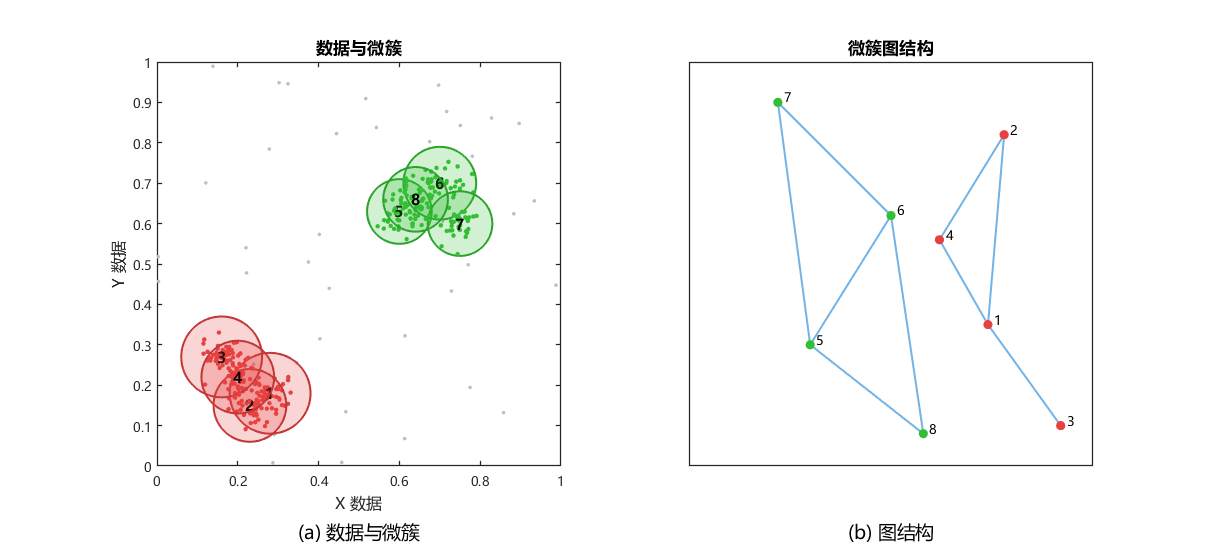
\includegraphics[width=0.85\textwidth]{images/chapter2/CEDAS}
	\caption{CEDAS微簇与图结构示意图}
	\label{fig_2_8_road}
\end{figure}

\subsubsection{CluStream}

CluStream 是经典的两阶段数据流聚类方法。在线阶段维护有限数量的微簇并持续更新其统计摘要；查询阶段再利用这些微簇执行宏聚类，例如通过 $k$-means 算法获得最终聚类结果。

该方法的优势在于在线计算开销较小，但宏簇输出依赖第二阶段重聚类操作，因此在需要高频输出时可能带来额外计算负担。



\subsubsection{DenStream}

DenStream 可以视为 CluStream 框架的密度扩展版本。其在线阶段维护两类微簇：

- 潜在微簇（potential micro-cluster）
- 离群微簇（outlier micro-cluster）

微簇权重随时间衰减，使长期缺乏新样本支持的结构逐渐消失，从而适应概念漂移。

宏簇输出阶段通常采用 DBSCAN 式密度连接，对潜在微簇中心进行聚合，从而能够刻画任意形状的簇结构。



\subsection{本章小结}

本章首先介绍了数据流聚类问题的基本特性与约束条件，并在此基础上给出了微簇摘要表示及其增量更新机制。随后对 CEDAS、CluStream 与 DenStream 三类典型方法进行了概述，为后续章节中面向地磁事件流的在线聚类方法设计提供了理论基础。


\chapter{基于节点状态自适应与场景概率判别的在线多车辆目标跟踪方法}
\label{chap:online_tracking}

\section{引言}

在单向双车道高速公路路段内，基于多地磁传感器的车辆目标跟踪系统会受到数据随机延迟到达、漏检以及噪声干扰等非理想因素的影响；同时，由于车辆行驶行为复杂，邻道干扰与双车长距离并行通过在上报量测的时空特性上又具有较强相似性，难以简单依据单条量测特征判断区分，从而影响车辆实时跟踪的准确性与稳定性。针对上述问题，本文面向系统常态工况下存在的量测到达时序错乱、短时漏检、噪声干扰以及复杂并行车况，提出一种基于节点状态自适应与场景概率判别的在线多车辆目标跟踪方法。

本章内容按照在线处理流程展开。首先，在量测进入关联与滤波之前，利用时间窗口缓存对量测到达时序进行矫正，并通过固定滞后窗口接纳迟到到达的量测，在必要时触发局部回放，从而提高轨迹可利用信息的完整性。其次，在量测时序矫正的基础上，建立与双车道地磁事件流相匹配的车辆运动模型与观测模型，给出状态初始化、状态预测与量测更新方法，形成统一的事件级状态估计框架。随后，围绕多车辆目标的数据关联问题，依次构建跟踪波门、关联似然与软关联权重计算方法，并结合节点检测概率与杂波强度的在线估计提升复杂工况下的关联鲁棒性；同时，针对邻道干扰与真实双车并行易混淆的问题，引入三状态场景判别模型，对局部交通场景进行概率解释。最后，在轨迹管理阶段，结合目标存在概率递推与基于场景后验的车道状态更新机制，实现轨迹的起始、确认、维持、删除以及车道状态修正，形成完整的在线跟踪流程。

\section{量测时序矫正}

多地磁传感器系统产生的是跨节点、异步到达的事件流。若直接按照数据到达顺序进行处理，则迟到量测会破坏事件真实发生的时间关系，进而影响后续状态预测、量测关联和轨迹维护。为此，本文首先对量测进行时间组织，并在有限滞后范围内允许迟到量测回插到历史扫描，从而保证进入后续状态估计与关联模块的数据尽可能满足时间一致性。

\subsection{时间窗口缓存与量测时序重排}

设单条地磁事件量测记为
\begin{equation}
	\mathbf z_j=\left(id_j,\,t_j,\,\ell_j,\,Mpeak_j,\ldots\right),
	\label{eq:ch3_event_def}
\end{equation}
其中，$id_j$ 为触发节点编号，$t_j$ 为事件触发时间戳，$\ell_j$ 为与该节点对应的边界车道线编号，$Mpeak_j$ 为地磁扰动峰值。为便于在线处理，将事件流按固定时间片 $\Delta T$ 组织为离散扫描序列。给定参考时刻 $t_0$，事件 $\mathbf z_j$ 所属的扫描序号定义为
\begin{equation}
	n(j)=\left\lfloor \frac{t_j-t_0}{\Delta T} \right\rfloor +1.
	\label{eq:ch3_scan_index}
\end{equation}
于是，第 $n$ 个扫描内的量测集合可写为
\begin{equation}
	\mathcal Z_n=
	\left\{
	\mathbf z_j\,\big|\, n(j)=n
	\right\}.
	\label{eq:ch3_scan_set}
\end{equation}

考虑到同一扫描内不同节点上报的量测仍可能存在到达顺序与真实触发顺序不一致的情况，本文在扫描内部再按触发时间戳升序进行排序，得到
\begin{equation}
	\mathcal Z_n^{\uparrow}=\mathrm{Sort}\left(\mathcal Z_n; t_j\uparrow\right).
	\label{eq:ch3_scan_sort}
\end{equation}
后续的状态预测、量测关联和轨迹更新均按照 $\mathcal Z_n^{\uparrow}$ 中的顺序逐条执行。由此，系统首先在扫描层面完成粗粒度时间对齐，再在扫描内部恢复事件的真实先后关系，为后续的事件级递推提供统一的时间组织基础。

\subsection{固定滞后窗口与局部回放}

仅依靠扫描内排序仍不足以解决迟到量测问题。当量测在其真实触发扫描已经处理完成后才到达系统时，若直接忽略该量测或将其并入当前扫描，都会破坏既有轨迹的时间一致性。为此，本文引入固定滞后窗口，对最近 $L$ 个扫描保持可回溯状态。定义时刻 $n$ 的活动窗口为
\begin{equation}
	\mathcal W_n=
	\left\{
	\mathcal Z_{n-L+1},\ldots,\mathcal Z_n
	\right\}.
	\label{eq:ch3_lag_window}
\end{equation}
同时，在窗口左端保留快照状态
\begin{equation}
	\mathcal S_{n-L}=
	\left\{
	\hat{\mathbf x}_{i,k|k},\mathbf P_{i,k|k},\gamma_i,
	\boldsymbol\pi_i^{\mathrm{lane}},
	\boldsymbol\pi_g^{\mathrm{scene}},
	\alpha_{D,b},\beta_{D,b},a_{\kappa,b},b_{\kappa,b}
	\right\},
	\label{eq:ch3_snapshot_reorg}
\end{equation}
其中分别包含轨迹状态与协方差、轨迹存在概率、车道后验、场景后验以及节点检测概率与杂波强度的后验参数。

当新到达量测 $\mathbf z_j$ 满足
\begin{equation}
	n(j)\in\{n-L+1,\ldots,n\},
	\label{eq:ch3_late_condition}
\end{equation}
则认为其属于固定滞后窗口内的迟到量测。此时，系统将该量测回插至对应历史扫描的量测集合中，并从快照 $\mathcal S_{n-L}$ 出发，按时间顺序重新执行窗口内的“状态预测--场景判别--数据关联--量测更新--轨迹管理”流程。若量测所属扫描早于窗口左端，则说明其已超出在线可修正范围，不再纳入本章在线跟踪流程，而留待后续离线分析或长缺测轨迹重构阶段处理。通过固定滞后窗口与局部回放机制，本文在有限计算复杂度下利用未来信息对近期历史关联进行修正，从而提高短时乱序与迟到条件下轨迹输出的稳定性与完整性。

在完成量测时序矫正后，系统获得了按真实时间顺序组织的事件流输入。下面在此基础上建立事件级车辆状态估计算法，为后续关联与场景判别提供统一的状态表达。

\section{基于双车道地磁传感器数据的车辆状态估计算法}
\label{sec:ch3_state_estimation}

经过时间组织后的地磁量测仍然是离散事件，而不是可直接递推的连续轨迹状态。因此，需要建立与事件流形式相匹配的车辆状态估计模型，将“车辆在某一时刻通过某一已知节点”这一事件事实转化为可用于滤波更新的状态约束。本节按照“模型建立--初始化--预测--更新”的顺序给出事件级状态估计算法。

\subsection{车辆运动模型与地磁事件观测模型}

由于双车道地磁系统并不直接提供车辆横向连续坐标，本文仅对车辆沿道路纵向的连续状态进行递推估计，而将横向安装位置、边界车道线编号和地磁扰动峰值等信息作为离散证据保留，用于后续的数据关联与车道状态判别。考虑到车辆在高速路段沿车道纵向行驶，且相邻地磁节点之间的通过时间通常处于较短时间尺度内，本文采用常速度（CV）模型作为车辆纵向运动的基础模型。设轨迹 $i$ 在第 $k$ 次有效更新后的状态向量为
\begin{equation}
	\mathbf x_{i,k}=
	\begin{bmatrix}
		p_{i,k}\\
		v_{i,k}
	\end{bmatrix},
	\label{eq:ch3_state_vec}
\end{equation}
其中，$p_{i,k}$ 与 $v_{i,k}$ 分别表示车辆在道路纵向上的位置与速度。

若轨迹 $i$ 在相邻两次有效更新之间的时间间隔为 $\Delta t_{i,k+1}$，则其状态转移模型写为
\begin{equation}
	\mathbf x_{i,k+1}=
	\mathbf F\left(\Delta t_{i,k+1}\right)\mathbf x_{i,k}+\mathbf w_{i,k},
	\label{eq:ch3_state_transition}
\end{equation}
其中，状态转移矩阵为
\begin{equation}
	\mathbf F\left(\Delta t_{i,k+1}\right)=
	\begin{bmatrix}
		1 & \Delta t_{i,k+1}\\
		0 & 1
	\end{bmatrix},
	\label{eq:ch3_F}
\end{equation}
过程噪声满足 $\mathbf w_{i,k}\sim\mathcal N(\mathbf 0,\mathbf Q(\Delta t_{i,k+1}))$。考虑短时机动和时间戳抖动对纵向传播误差的影响，过程噪声协方差写为
\begin{equation}
	\mathbf Q\left(\Delta t_{i,k+1}\right)
	=
	q_a
	\begin{bmatrix}
		\dfrac{\Delta t_{i,k+1}^{4}}{4} & \dfrac{\Delta t_{i,k+1}^{3}}{2}\\[6pt]
		\dfrac{\Delta t_{i,k+1}^{3}}{2} & \Delta t_{i,k+1}^{2}
	\end{bmatrix}
	+
	\begin{bmatrix}
		\gamma_t \hat v_{i,k+1|k}^{\,2}\sigma_t^2 & 0\\
		0 & 0
	\end{bmatrix}.
	\label{eq:ch3_Q}
\end{equation}

当地磁事件最终被关联到轨迹后，事件“车辆在时刻 $t_j$ 通过节点 $id_j$”这一事实可转化为纵向位置约束。记节点 $id_j$ 的纵向安装坐标为 $x_{id_j}$，则定义伪位置观测
\begin{equation}
	\tilde p_{i,k+1}=x_{id_j}.
	\label{eq:ch3_pseudo_meas}
\end{equation}
相应的观测模型写为
\begin{equation}
	\tilde p_{i,k+1}=\mathbf H\mathbf x_{i,k+1}+e_{i,k+1},
	\qquad
	\mathbf H=
	\begin{bmatrix}
		1 & 0
	\end{bmatrix},
	\qquad
	e_{i,k+1}\sim\mathcal N(0,R_{id_j}),
	\label{eq:ch3_measurement_k}
\end{equation}
其中，$R_{id_j}$ 为与节点 $id_j$ 相关的观测方差。需要说明的是，$R_{id_j}$ 反映的是节点触发区间宽度、安装标定误差以及节点工作状态不稳定性折算到位置约束上的不确定性，而不是时间戳误差方差。后文将根据节点检测概率与杂波强度的在线估计结果，对 $R_{id_j}$ 进行自适应调整。

\subsection{状态初始化}

新生轨迹只对当前扫描中未被任何已确认轨迹吸收的量测执行初始化，而不会反过来参与当前时刻已有轨迹的关联竞争。设事件 $\mathbf z_{j_0}$ 触发了新候选轨迹 $i$，则其初始位置取为对应节点的纵向坐标
\begin{equation}
	p_{i,0}=x_{id_{j_0}}.
	\label{eq:ch3_init_pos}
\end{equation}
由于单条地磁事件无法可靠提供速度信息，本文采用道路历史平均速度或经验速度 $\bar v_0$ 作为初始速度先验，从而得到初始状态均值
\begin{equation}
	\hat{\mathbf x}_{i,0|0}=
	\begin{bmatrix}
		p_{i,0}\\
		\bar v_0
	\end{bmatrix}.
	\label{eq:ch3_init_state}
\end{equation}
对应的初始协方差取为
\begin{equation}
	\mathbf P_{i,0|0}=\mathrm{diag}\left(\sigma_{p0}^{2},\sigma_{v0}^{2}\right),
	\label{eq:ch3_init_cov}
\end{equation}
其中，$\sigma_{p0}^{2}$ 与节点位置观测方差同量级，$\sigma_{v0}^{2}$ 取较大的先验值，以反映新生轨迹在初始阶段速度不确定性较高。

为使地磁扰动峰值信息能够进入后续关联计算，本文同时维护轨迹级对数磁峰值统计量。设新生事件的对数峰值为
\begin{equation}
	m_{i,0}=\log(Mpeak_{j_0}+\varepsilon_M),
	\label{eq:ch3_init_mag}
\end{equation}
则初始化其磁特征均值与方差为
\begin{equation}
	\mu_{i,0}^{M}=m_{i,0},
	\qquad
	(\sigma_{i,0}^{M})^{2}=\sigma_{M0}^{2}.
	\label{eq:ch3_init_mag_stat}
\end{equation}
这样设置的目的在于，使新生轨迹除了具备位置与速度先验外，还保留可供后续关联使用的地磁特征先验。

\subsection{状态预测}

设轨迹 $i$ 在第 $k$ 次有效更新后的后验状态均值与协方差分别为
\begin{equation}
	\hat{\mathbf x}_{i,k|k},
	\qquad
	\mathbf P_{i,k|k}.
	\label{eq:ch3_post_state}
\end{equation}
若后续某条事件最终对应其第 $k+1$ 次有效更新，则该事件触发时间记为 $t_j$，相邻两次有效更新之间的时间间隔定义为
\begin{equation}
	\Delta t_{i,k+1}=t_j-t_{i,k}.
	\label{eq:ch3_dt_update}
\end{equation}
于是，轨迹 $i$ 在第 $k+1$ 次更新前的预测状态均值与预测协方差分别为
\begin{equation}
	\hat{\mathbf x}_{i,k+1|k}
	=
	\mathbf F\left(\Delta t_{i,k+1}\right)\hat{\mathbf x}_{i,k|k},
	\label{eq:ch3_predict_state}
\end{equation}
\begin{equation}
	\mathbf P_{i,k+1|k}
	=
	\mathbf F\left(\Delta t_{i,k+1}\right)
	\mathbf P_{i,k|k}
	\mathbf F^{\mathrm T}\left(\Delta t_{i,k+1}\right)
	+
	\mathbf Q\left(\Delta t_{i,k+1}\right).
	\label{eq:ch3_predict_cov}
\end{equation}
由此可将轨迹状态传播到候选事件触发时刻，为后续量测关联和滤波更新提供统一的预测先验。

\subsection{量测更新}

若轨迹 $i$ 最终被分配到事件 $\mathbf z_j$，则由伪位置观测模型可得创新为
\begin{equation}
	\nu_{i,k+1}=\tilde p_{i,k+1}-\mathbf H\hat{\mathbf x}_{i,k+1|k},
	\label{eq:ch3_innovation_event}
\end{equation}
对应的创新方差为
\begin{equation}
	S_{i,k+1}=\mathbf H\mathbf P_{i,k+1|k}\mathbf H^{\mathrm T}+R_{id_j}.
	\label{eq:ch3_S_event}
\end{equation}
于是，Kalman 增益写为
\begin{equation}
	\mathbf K_{i,k+1}
	=
	\mathbf P_{i,k+1|k}\mathbf H^{\mathrm T}
	\left(
	\mathbf H\mathbf P_{i,k+1|k}\mathbf H^{\mathrm T}+R_{id_j}
	\right)^{-1},
	\label{eq:ch3_K_event}
\end{equation}
相应的状态均值与协方差更新为
\begin{equation}
	\hat{\mathbf x}_{i,k+1|k+1}
	=
	\hat{\mathbf x}_{i,k+1|k}
	+
	\mathbf K_{i,k+1}\nu_{i,k+1},
	\label{eq:ch3_update_state_event}
\end{equation}
\begin{equation}
	\mathbf P_{i,k+1|k+1}
	=
	\left(\mathbf I-\mathbf K_{i,k+1}\mathbf H\right)\mathbf P_{i,k+1|k}.
	\label{eq:ch3_update_cov_event}
\end{equation}
若轨迹在当前扫描内未获得有效关联，则不执行量测更新，而仅保留预测结果，并将该次未命中事实作为后续目标存在概率递推和节点检测概率统计更新的输入证据。至此，本文建立了与地磁事件流相匹配的事件级状态估计框架。下面进一步解决多车辆共享事件流条件下的量测归属与场景消歧问题。

\section{多车辆目标数据关联与并行场景判别}
\label{sec:ch3_association}

在完成车辆状态估计模型之后，下一步需要处理事件流中的量测来源不确定性问题。对于双车道地磁系统而言，量测归属不仅取决于时间一致性，还受到节点检测能力差异、杂波水平变化以及邻道干扰与真实双车并行混淆的共同影响。因此，本节围绕跟踪波门、关联似然与软关联权重、节点状态自适应以及并行场景判别四个方面构建统一的概率建模框架。

\subsection{跟踪波门设置}

由于地磁量测在时间轴上异步到达，系统无法像同步采样传感器那样在单一采样时刻统一判断所有事件的来源。因此，本文首先基于时间一致性构造轨迹门控。对任意候选事件 $\mathbf z_j$，记其触发节点编号为 $id_j$，对应节点的纵向安装坐标为 $x_{id_j}$，触发时间戳为 $t_j$。若轨迹 $i$ 在当前状态下可能继续前进至该节点，则由常速度模型可得到其预测通过节点 $id_j$ 的时刻
\begin{equation}
	\hat t_{i\rightarrow id_j}
	=
	t_{i,k}+\frac{x_{id_j}-\hat p_{i,k|k}}{\hat v_{i,k|k}}.
	\label{eq:ch3_pred_time}
\end{equation}
于是，事件 $\mathbf z_j$ 与轨迹 $i$ 之间的时间残差定义为
\begin{equation}
	\nu^{t}_{i,j}=t_j-\hat t_{i\rightarrow id_j}.
	\label{eq:ch3_time_residual}
\end{equation}
由式~\eqref{eq:ch3_pred_time} 对状态变量 $(p,v)$ 作一阶线性化，可得雅可比向量
\begin{equation}
	\mathbf J_{i,j}
	=
	\begin{bmatrix}
		-\dfrac{1}{\hat v_{i,k|k}} & -\dfrac{x_{id_j}-\hat p_{i,k|k}}{\hat v_{i,k|k}^{\,2}}
	\end{bmatrix},
	\label{eq:ch3_time_jacobian}
\end{equation}
从而时间残差方差写为
\begin{equation}
	S^{t}_{i,j}=\mathbf J_{i,j}\mathbf P_{i,k|k}\mathbf J_{i,j}^{\mathrm T}+\sigma_{t,id_j}^{2},
	\label{eq:ch3_time_var}
\end{equation}
其中，$\sigma_{t,id_j}^{2}$ 表示节点 $id_j$ 的时间戳误差方差。基于此，定义时间域归一化距离
\begin{equation}
	d^{t\,2}_{i,j}=\frac{\left(\nu^{t}_{i,j}\right)^2}{S^{t}_{i,j}}.
	\label{eq:ch3_time_maha}
\end{equation}
当 $d^{t\,2}_{i,j}\le \gamma_t$ 时，认为事件 $\mathbf z_j$ 落入轨迹 $i$ 的时间门控范围内，其中 $\gamma_t$ 为时间门控阈值。对应的门控宽度可写为
\begin{equation}
	V^{t}_{i,j}=2\sqrt{\gamma_t S^{t}_{i,j}}.
	\label{eq:ch3_gate_width_time}
\end{equation}
该门控机制为后续关联求解提供了候选事件集合，并显著降低了不合理匹配进入关联阶段的概率。

\subsection{关联似然建模与软关联权重计算}

在跟踪波门筛选出候选事件之后，本文进一步构造融合运动学一致性、地磁扰动峰值一致性和车道/场景一致性的关联似然。对轨迹 $i$ 与事件 $\mathbf z_j$，定义总似然为
\begin{equation}
	g(\mathbf z_j\mid \hat{\mathbf x}_{i,k|k})
	=
	g_{i,j}^{\mathrm{time}}
	\phi_{i,j}^{\mathrm{mag}}
	\phi_{i,j}^{\mathrm{lane}},
	\label{eq:ch3_total_likelihood}
\end{equation}
其中，基于时间残差的运动学一致性项为
\begin{equation}
	g_{i,j}^{\mathrm{time}}
	=
	\frac{1}{\sqrt{2\pi S^{t}_{i,j}}}
	\exp\left(-\frac{1}{2}d^{t\,2}_{i,j}\right),
	\label{eq:ch3_g_time}
\end{equation}
地磁扰动峰值一致性项采用轨迹历史对数峰值统计建模：
\begin{equation}
	\phi_{i,j}^{\mathrm{mag}}
	=
	\exp\left[
	-\frac{
		\left(
		\log(Mpeak_j+\varepsilon_M)-\mu_i^{M}
		\right)^2
	}{2\left((\sigma_i^{M})^2+\varepsilon_M\right)}
	\right],
	\label{eq:ch3_phi_mag}
\end{equation}
车道/场景一致性项定义为
\begin{equation}
	\phi_{i,j}^{\mathrm{lane}}
	=
	\sum_{\beta\in\{1,2\}}
	p\!\left(\ell_j\middle|\beta,\boldsymbol\pi_{g(j),n}^{\mathrm{scene}}\right)
	\pi_{i,n}^{\mathrm{lane}}(\beta),
	\label{eq:ch3_phi_lane}
\end{equation}
其中，$g(j)$ 表示事件 $\mathbf z_j$ 所属的左右节点对编号。

为使不同节点、不同车流密度和不同杂波条件下的关联代价具有可比性，本文采用显式包含节点检测概率与节点杂波强度的标准化关联似然比。记事件 $\mathbf z_j$ 所属节点 $id_j$ 在扫描 $n$ 开始时冻结的检测概率后验均值和杂波强度后验均值分别为 $\hat p_D^{(id_j)}(n^-)$ 与 $\hat\kappa_{id_j}(n^-)$，则定义
\begin{equation}
	\Lambda_{i,j}(n)
	=
	\frac{\hat p_D^{(id_j)}(n^-)\,g(\mathbf z_j\mid \hat{\mathbf x}_{i,k|k})}{\hat\kappa_{id_j}(n^-)},
	\label{eq:ch3_assoc_ratio}
\end{equation}
相应的全局分配代价写为
\begin{equation}
	C_{i,j}(n)=-\log \Lambda_{i,j}(n).
	\label{eq:ch3_assoc_cost}
\end{equation}

进一步地，为向节点后验更新和目标存在概率更新提供软统计证据，对每条轨迹 $i$ 在其验证门内定义局部软关联权重。设轨迹 $i$ 在扫描 $n$ 中的候选事件集合为 $\mathcal G_i(n)$，则对任意 $\mathbf z_j\in\mathcal G_i(n)$，定义
\begin{equation}
	\beta_{i,j}(n)=
	\frac{\Lambda_{i,j}(n)}{1-\bar p_{D,i}(n)P_G+\sum\limits_{\mathbf z_\ell\in\mathcal G_i(n)}\Lambda_{i,\ell}(n)},
	\label{eq:ch3_beta_soft}
\end{equation}
对应的未检出权重为
\begin{equation}
	\beta_{i,0}(n)=
	\frac{1-\bar p_{D,i}(n)P_G}{1-\bar p_{D,i}(n)P_G+\sum\limits_{\mathbf z_\ell\in\mathcal G_i(n)}\Lambda_{i,\ell}(n)}.
	\label{eq:ch3_beta_miss}
\end{equation}
式中，$\bar p_{D,i}(n)$ 表示轨迹 $i$ 在当前扫描预测对应节点上的平均检测概率，$P_G$ 表示时间门控概率。本文在工程实现上保留“全局分配 + 局部补关联”的总体骨架，而式~\eqref{eq:ch3_beta_soft} 与式~\eqref{eq:ch3_beta_miss} 则用于构造软统计量，供后续节点状态在线估计与目标存在概率递推使用。

\subsection{节点检测概率与杂波强度在线估计}
\label{subsec:ch3_node_stats}

在关联似然建立之后，还需要根据已经发生的事件对节点检测能力和杂波水平进行在线修正。由于当前扫描的关联结果本身依赖节点后验，因此若在同一扫描中立即利用本扫描结果反向更新节点参数，会引入明显的循环依赖。为此，本文采用“扫描冻结 + 定稿后更新”的两阶段策略。

具体地，在扫描 $n$ 开始时，先冻结全体节点的检测概率与杂波强度后验均值，记为
\begin{equation}
	\Theta_n^{-}=
	\left\{
	\hat p_D^{(b)}(n^-),\hat\kappa_b(n^-):b\in\mathcal B
	\right\},
	\label{eq:ch3_theta_frozen}
\end{equation}
其中，$\mathcal B$ 表示节点集合。扫描 $n$ 内的全部门控、关联和轨迹管理均使用 $\Theta_n^{-}$ 完成，而不会在处理中途改变节点参数。只有当某一扫描在固定滞后窗口回放之后被正式定稿时，才利用该扫描的软统计量更新节点后验。

对节点 $b$ 的检测概率，采用 Beta 先验建模：
\begin{equation}
	p_D^{(b)}\sim \mathrm{Beta}\bigl(\alpha_{D,b},\beta_{D,b}\bigr),
	\label{eq:ch3_beta_prior}
\end{equation}
对节点 $b$ 的杂波强度，采用 Gamma 先验建模：
\begin{equation}
	\kappa_b\sim \mathrm{Gamma}\bigl(a_{\kappa,b},b_{\kappa,b}\bigr),
	\label{eq:ch3_gamma_prior}
\end{equation}
其中，Gamma 分布采用形状--率参数化，其数学期望为
\begin{equation}
	\mathbb E[\kappa_b]=\frac{a_{\kappa,b}}{b_{\kappa,b}}.
	\label{eq:ch3_kappa_mean}
\end{equation}

设扫描 $m$ 完成固定滞后回放并被定稿后，定义节点 $b$ 在该扫描上的高置信通过轨迹集合为 $\mathcal E_b(m)$。集合中的轨迹满足其存在概率超过阈值 $\tau_E$，并且按预测状态在扫描 $m$ 内与节点 $b$ 具有可达一致性。记轨迹 $i\in\mathcal E_b(m)$ 对节点 $b$ 的通过机会指示为
\begin{equation}
	\omega_{i,b}(m)=\mathbb I\left\{d^{t\,2}_{i,b}(m)\le \gamma_t\right\},
	\label{eq:ch3_pass_indicator}
\end{equation}
则节点 $b$ 在扫描 $m$ 上的软命中计数和软期望计数分别定义为
\begin{equation}
	N_{\mathrm{hit}}^{(b)}(m)
	=
	\sum_{i\in\mathcal E_b(m)}
	\omega_{i,b}(m)
	\sum_{\mathbf z_j\in \mathcal Z_m:id_j=b}
	\beta_{i,j}(m),
	\label{eq:ch3_soft_hit}
\end{equation}
\begin{equation}
	N_{\mathrm{exp}}^{(b)}(m)
	=
	\sum_{i\in\mathcal E_b(m)}
	\omega_{i,b}(m).
	\label{eq:ch3_soft_exp}
\end{equation}
据此，节点检测概率的后验递推写为
\begin{equation}
	\alpha_{D,b}(m)=\lambda_D\alpha_{D,b}(m-1)+N_{\mathrm{hit}}^{(b)}(m),
	\qquad
	\beta_{D,b}(m)=\lambda_D\beta_{D,b}(m-1)+N_{\mathrm{exp}}^{(b)}(m)-N_{\mathrm{hit}}^{(b)}(m),
	\label{eq:ch3_beta_update}
\end{equation}
其中，$\lambda_D\in(0,1]$ 为遗忘因子。相应的检测概率后验均值为
\begin{equation}
	\hat p_D^{(b)}(m)=\frac{\alpha_{D,b}(m)}{\alpha_{D,b}(m)+\beta_{D,b}(m)}.
	\label{eq:ch3_pD_mean}
\end{equation}

对于节点杂波强度，利用未被任何轨迹解释的软剩余概率构造软杂波计数：
\begin{equation}
	N_{\mathrm{clu}}^{(b)}(m)
	=
	\sum_{\mathbf z_j\in \mathcal Z_m:id_j=b}
	\left[1-\sum_{i\in\mathcal E_b(m)}\beta_{i,j}(m)\right],
	\label{eq:ch3_soft_clutter}
\end{equation}
对应的总暴露时间门控宽度定义为
\begin{equation}
	V_b(m)=
	\sum_{i\in\mathcal E_b(m)}
	\omega_{i,b}(m)V^{t}_{i,b}(m),
	\label{eq:ch3_exposure_volume}
\end{equation}
于是，节点杂波强度的后验递推为
\begin{equation}
	a_{\kappa,b}(m)=\lambda_{\kappa}a_{\kappa,b}(m-1)+N_{\mathrm{clu}}^{(b)}(m),
	\qquad
	b_{\kappa,b}(m)=\lambda_{\kappa}b_{\kappa,b}(m-1)+V_b(m),
	\label{eq:ch3_kappa_update}
\end{equation}
对应的杂波强度后验均值为
\begin{equation}
	\hat\kappa_b(m)=\frac{a_{\kappa,b}(m)}{b_{\kappa,b}(m)}.
	\label{eq:ch3_kappa_mean_v2}
\end{equation}

进一步地，将节点后验传递到位置更新的观测方差中，定义
\begin{equation}
	R_b(n)=R_0\left[1+c_D\bigl(1-\hat p_D^{(b)}(n)\bigr)+c_{\kappa}\hat\kappa_b(n)\right],
	\label{eq:ch3_Rb}
\end{equation}
其中，$R_0$ 为基准观测方差，$c_D$ 和 $c_{\kappa}$ 为调节系数。式~\eqref{eq:ch3_Rb} 表明：当节点检测概率下降或节点杂波强度升高时，其观测方差自动增大，从而降低该节点量测对状态更新的牵引强度。

\subsection{邻道干扰与双车并行场景判别模型}

在节点状态在线估计之后，还需要进一步解决双车道场景中最难区分的一类情况，即邻道干扰与真实双车并行的混淆。现有规则系统通常依赖单次时间差阈值和磁峰值比值来区分这两类情形，但在真实道路中确实存在少量两车长时间并行且相对时间差持续较小的情况，此时若仅依赖单帧规则，系统容易把真实双车并行误判为邻道干扰。

为此，本文显式引入场景状态变量
\begin{equation}
	s_{g,n}\in\left\{\mathcal I_1,\mathcal I_2,\mathcal P\right\},
	\label{eq:ch3_scene_state}
\end{equation}
其中，$\mathcal I_1$ 表示“1车道真实车辆、2车道为邻道干扰”，$\mathcal I_2$ 表示“2车道真实车辆、1车道为邻道干扰”，$\mathcal P$ 表示“真实双车并行”。对节点对 $g$ 在扫描 $n$ 的场景后验概率向量记为
\begin{equation}
	\boldsymbol\pi_{g,n}^{\mathrm{scene}}=
	\begin{bmatrix}
		\pi_{g,n}^{\mathrm{scene}}(\mathcal I_1) &
		\pi_{g,n}^{\mathrm{scene}}(\mathcal I_2) &
		\pi_{g,n}^{\mathrm{scene}}(\mathcal P)
	\end{bmatrix}.
	\label{eq:ch3_scene_vector}
\end{equation}
采用一阶马尔可夫模型描述场景转移，则预测步写为
\begin{equation}
	\boldsymbol\pi_{g,n|n-1}^{\mathrm{scene}}=
	\boldsymbol\pi_{g,n-1|n-1}^{\mathrm{scene}}\mathbf A_s,
	\label{eq:ch3_scene_predict}
\end{equation}
其中
\begin{equation}
	\mathbf A_s=
	\begin{bmatrix}
		1-\lambda_c-\rho_{1P} & \lambda_c & \rho_{1P}\\
		\lambda_c & 1-\lambda_c-\rho_{2P} & \rho_{2P}\\
		\rho_{P1} & \rho_{P2} & 1-\rho_{P1}-\rho_{P2}
	\end{bmatrix}.
	\label{eq:ch3_As}
\end{equation}

在观测层面，提取如下场景观测向量：
\begin{equation}
	\mathbf o_{g,n}=
	\begin{bmatrix}
		\Delta t_{g,n}^{\mathrm{adj}} &
		\alpha_{g,n} &
		e_{g,n}^{\mathrm{opp}} &
		d_{g,n,\mathrm{opp}}^2
	\end{bmatrix}^{\mathrm T},
	\label{eq:ch3_scene_obs}
\end{equation}
其中，$\Delta t_{g,n}^{\mathrm{adj}}$ 表示左右两侧节点触发时间差，$\alpha_{g,n}$ 表示两侧地磁扰动峰值对数比值，$e_{g,n}^{\mathrm{opp}}\in\{0,1\}$ 表示对侧是否存在触发，$d_{g,n,\mathrm{opp}}^2$ 表示对侧触发被另一车道现有轨迹解释的最小时间域门控距离。若对侧不存在可解释轨迹，则令 $d_{g,n,\mathrm{opp}}^2=d_0^2$，其中 $d_0^2$ 为较大的常数。

采用条件独立近似构造场景观测似然：
\begin{equation}
	p(\mathbf o_{g,n}\mid s_{g,n})
	=
	p(\Delta t_{g,n}^{\mathrm{adj}}\mid s_{g,n})\,
	p(\alpha_{g,n}\mid s_{g,n})\,
	p(e_{g,n}^{\mathrm{opp}}\mid s_{g,n})\,
	p(d_{g,n,\mathrm{opp}}^2\mid s_{g,n}),
	\label{eq:ch3_scene_likelihood}
\end{equation}
从而场景后验递推为
\begin{equation}
	\pi_{g,n|n}^{\mathrm{scene}}(s)
	=
	\frac{p(\mathbf o_{g,n}\mid s)\,\pi_{g,n|n-1}^{\mathrm{scene}}(s)}{\sum\limits_{s'\in\{\mathcal I_1,\mathcal I_2,\mathcal P\}}p(\mathbf o_{g,n}\mid s')\,\pi_{g,n|n-1}^{\mathrm{scene}}(s')},
	\qquad s\in\{\mathcal I_1,\mathcal I_2,\mathcal P\}.
	\label{eq:ch3_scene_update}
\end{equation}
该模型的关键意义在于：它不再依赖单帧时间差阈值，而是利用多步时序信息持续判断对侧触发更像是邻道干扰还是另一条真实轨迹的连续观测，从而为后续轨迹级车道状态更新提供更稳定的场景解释。

\section{轨迹管理与车道状态在线判别}
\label{sec:ch3_track_management}

经过状态估计、数据关联和场景判别之后，系统已经获得“当前量测属于哪条轨迹”以及“当前局部场景更可能是哪一种”的概率解释。为了持续输出身份一致且车道状态稳定的在线轨迹，还需要进一步完成轨迹起始、存在概率递推、删除决策以及基于场景后验的车道状态更新。

\subsection{轨迹起始与确认}

当扫描 $n$ 中存在未被任何已确认轨迹吸收的量测，或者其与所有已确认轨迹的关联似然比均低于阈值 $\Lambda_{\min}$ 时，系统以该量测触发新候选轨迹。候选轨迹仅记录首条量测、初始车道证据和初始场景上下文，不立即输出。为抑制杂波触发假轨迹，本文采用 $M/N$ 确认策略：若候选轨迹在最近 $N$ 个扫描内获得至少 $M$ 次有效关联，且其平均关联似然比不低于给定阈值，则转为已确认轨迹；否则在超过 $N$ 个扫描仍未满足条件时予以删除。

与仅依赖命中计数的规则不同，本文对候选轨迹的确认同时考察运动学一致性、节点可靠性和场景一致性。当候选轨迹主要由高杂波节点触发，或其长期处于“邻道干扰概率占优”的场景后验下时，即使短时获得若干次命中，也不会立即提升为已确认状态。只有当其在多步时序上能稳定维持较高的关联似然比和存在概率时，才执行确认。

\subsection{目标存在概率更新与删除策略}

为避免轨迹因单次未检出而立即终止，本文显式维护每条轨迹的存在概率 $\gamma_{t,n}$。设轨迹 $t$ 在第 $n$ 次扫描前的存在概率预测值为 $\gamma_{t,n|n-1}$，则其递推写为
\begin{equation}
	\gamma_{t,n|n-1}=p_S\gamma_{t,n-1|n-1}+p_B\left(1-\gamma_{t,n-1|n-1}\right),
	\label{eq:ch3_exist_predict_v2}
\end{equation}
其中，$p_S$ 为轨迹存活概率，$p_B$ 为新生概率。

若轨迹 $t$ 在扫描 $n$ 中通过全局分配被分配到量测 $\mathbf z_j$，则用标准化关联似然比完成存在概率更新：
\begin{equation}
	\gamma_{t,n|n}=
	\frac{\Lambda_{t,j}(n)\gamma_{t,n|n-1}}{\Lambda_{t,j}(n)\gamma_{t,n|n-1}+1-\gamma_{t,n|n-1}}.
	\label{eq:ch3_exist_hit_v2}
\end{equation}
若轨迹在当前扫描中未获得有效关联，则利用预测对应节点上的平均检测概率完成未检出更新：
\begin{equation}
	\gamma_{t,n|n}=
	\frac{\left[1-\bar p_{D,t}(n)P_G\right]\gamma_{t,n|n-1}}{\left[1-\bar p_{D,t}(n)P_G\right]\gamma_{t,n|n-1}+1-\gamma_{t,n|n-1}}.
	\label{eq:ch3_exist_miss_v2}
\end{equation}
在工程实现中，存在概率与连续漏检计数联合用于轨迹维持与删除。设连续漏检计数为 $N_{\mathrm{miss}}(t)$，则当
\begin{equation}
	\gamma_{t,n|n}<\gamma_{\mathrm{del}}
	\qquad\text{或}\qquad
	N_{\mathrm{miss}}(t)>N_{\mathrm{del}},
	\label{eq:ch3_delete_v2}
\end{equation}
时，判定轨迹终止。这里，$N_{\mathrm{del}}$ 需与固定滞后窗口长度 $L$ 协同设置：当 $N_{\mathrm{miss}}(t)\le L$ 时，系统优先等待局部回放结果；当连续缺测长度超过 $L$ 且存在概率持续下降时，说明当前在线方法已难以可靠维持身份一致性，此时将轨迹转为轨迹片段并交由下一章进一步拼接。

\subsection{基于场景后验的车道状态更新与修正}

场景概率判别解决的是“当前量测对应的是哪种局部交通场景”，而轨迹级车道状态更新解决的是“某条轨迹当前属于哪条车道以及是否需要进行车道状态修正”。虽然地磁系统无法直接给出车辆横向连续位置，但量测携带的边界车道线编号仍提供了稳定的离散车道证据。设轨迹 $t$ 在第 $n$ 次扫描时的车道状态为 $c_{t,n}\in\{1,2\}$，其车道后验概率向量记为
\begin{equation}
	\boldsymbol\pi_{t,n}^{\mathrm{lane}}=
	\begin{bmatrix}
		\pi_{t,n}^{\mathrm{lane}}(1) &
		\pi_{t,n}^{\mathrm{lane}}(2)
	\end{bmatrix}.
	\label{eq:ch3_lane_vector_v2}
\end{equation}
预测步采用两状态马尔可夫模型：
\begin{equation}
	\boldsymbol\pi_{t,n|n-1}^{\mathrm{lane}}
	=
	\boldsymbol\pi_{t,n-1|n-1}^{\mathrm{lane}}
	\begin{bmatrix}
		1-p_c & p_c\\
		p_c & 1-p_c
	\end{bmatrix},
	\label{eq:ch3_lane_predict_v2}
\end{equation}
其中，$p_c$ 为单步换道概率。

若轨迹 $t$ 在当前扫描中关联到量测 $\mathbf z_j$，则其车道后验按 Bayes 规则更新：
\begin{equation}
	\pi_{t,n|n}^{\mathrm{lane}}(\beta)
	=
	\frac{p(\ell_j\mid \beta,\boldsymbol\pi_{g(j),n}^{\mathrm{scene}})\pi_{t,n|n-1}^{\mathrm{lane}}(\beta)}{\sum\limits_{\beta'=1}^{2}p(\ell_j\mid \beta',\boldsymbol\pi_{g(j),n}^{\mathrm{scene}})\pi_{t,n|n-1}^{\mathrm{lane}}(\beta')},
	\qquad \beta\in\{1,2\}.
	\label{eq:ch3_lane_update_v2}
\end{equation}
当轨迹未获得关联时，保持预测结果不变。由于式~\eqref{eq:ch3_lane_update_v2} 将场景后验显式纳入车道更新过程，因此系统在邻道高干扰时不会仅凭一次对侧触发就轻易切换车道，而在真实双车并行和稳定换道阶段又能够逐步累积正确证据。

在输出层面，本文采用稳定性优先原则。当某一车道后验概率连续多次超过阈值 $\tau_{\mathrm{lane}}$ 且持续时间超过 $T_{\mathrm{lane}}$ 时，输出该车道；当两车道后验发生持续且显著翻转时，判定换道事件，并将换道时刻对齐到固定滞后窗口提交的最早扫描，以降低单帧波动对换道时刻标注的影响。

\subsection{算法流程汇总}

综合上述各节，本章在线多车辆目标跟踪方法在每个扫描周期的主要处理流程如下：
\begin{enumerate}
	\item 接收异步地磁事件流，并按时间片 $\Delta T$ 组织为扫描量测集合；在扫描内部按触发时间戳升序重排，形成时间一致的量测处理序列；
	\item 对新到达量测判断其是否属于固定滞后窗口，若属于窗口内迟到量测，则将其回插到对应历史扫描，并从窗口左端快照出发执行局部回放；
	\item 对所有活动轨迹执行状态预测，得到候选事件触发时刻的预测状态及其不确定性；
	\item 基于预测触发时间与实际触发时间构造时间域跟踪波门，筛选候选轨迹--量测对；
	\item 对门内候选对计算关联似然与标准化关联代价，并结合节点检测概率、杂波强度以及软关联权重完成多轨迹事件归属；
	\item 根据当前扫描的双侧触发模式、时间差和地磁扰动峰值等信息更新邻道干扰/双车并行三状态场景后验；
	\item 对获得有效关联的轨迹执行量测更新，对未获得关联的轨迹更新目标存在概率，并根据规则完成轨迹的起始、确认、维持与删除；
	\item 利用场景后验和边界车道线编号对轨迹车道状态进行在线更新与修正，并在满足条件时输出换道事件；
	\item 当窗口左端扫描不再可能受更早迟到量测影响时，将其定稿并利用该扫描的软统计量更新节点检测概率与杂波强度后验，然后将其移出活动窗口。
\end{enumerate}

通过上述处理流程，系统能够在量测乱序、短时漏检、节点状态变化以及邻道干扰与双车并行易混淆等复杂条件下，持续输出较为连续且身份一致的车辆轨迹，并为后续实验验证提供完整的方法实现基础。

\section{实验设计与结果分析}
\label{sec:ch3_experiment}

\subsection{实验目的与验证点}

本章实验围绕“标准化关联的有效性”“节点后验的稳定性”“场景判别能力”“漏检容忍边界”和“在线实时性”五个问题展开，重点验证以下内容：
\begin{enumerate}
	\item 显式引入检测概率、量测似然和杂波强度后，关联代价在不同车流密度和杂波水平下是否比规则打分更稳定；
	\item 节点检测概率与节点杂波强度的“冻结参数—软计数—窗口定稿后更新”策略是否能够避免错误自强化；
	\item 三状态场景判别是否能够在邻道干扰和真实双车并行场景下减少误关联和车道判别抖动；
	\item 本章方法对轻度漏检和短连漏检的稳定容忍范围是多少，其失效边界如何自然引出第~4~章的轨迹片段在线聚类；
	\item 在保持现有系统主干不变的前提下，所提方法是否满足在线运行要求。
\end{enumerate}

\subsection{数据集、实验平台与预处理}

本章实验所使用的实测数据来源于双车道地磁检测系统采集的两天事件流数据，分别记为 \texttt{streamIn1215} 与 \texttt{streamIn1216}。两份数据均为按事件触发记录的异步原始流，每条记录至少包含触发时间戳 \texttt{date}、入队时间 \texttt{inQueueTime}、车道编号 \texttt{lane}、节点编号 \texttt{devSort}、地磁峰值 \texttt{geomPeak} 以及事件持续时长 \texttt{timeLength} 等字段。由于原始事件流仅反映节点级触发过程，并不包含车辆级真值轨迹 ID、真实场景标签以及完整的连续漏检标注，因此其不能直接支撑场景判别准确率、身份切换次数、轨迹碎片数等监督指标的精确统计。

基于上述特点，本文将 \texttt{streamIn1215} 与 \texttt{streamIn1216} 作为本章实验的唯一实测数据源，但其作用主要体现在\textbf{经验统计标定}而非直接作为全部评测样本。具体而言，首先分别按车道统计地磁峰值 $\texttt{geomPeak}$ 与事件持续时长 $\texttt{timeLength}$ 的经验分布，用于刻画不同车道下地磁响应强度与触发持续时间的统计特征；其次，利用到达延迟
\[
\Delta t_{\mathrm{delay}}=\texttt{inQueueTime}-\texttt{date}
\]
的经验分布刻画异步通信与系统缓冲带来的时间乱序特性；最后，结合节点编号 \texttt{devSort} 与双车道节点布设关系，将原始事件流映射为后续仿真器中的节点拓扑、车道结构及时间组织参数。

在完成上述经验统计标定后，本文进一步构造与实测数据统计特性一致的可控仿真事件流。仿真器沿道路纵向按照实地系统一致的双车道节点拓扑进行布设，车辆到达过程、纵向运行速度、磁峰值幅度、事件持续时长以及迟到量测扰动均由实测数据标定结果驱动生成。同时，在仿真过程中可按需注入连续漏检、邻道干扰、双车并行、节点退化、虚警事件和迟到量测等非理想因素，从而获得带有完整车辆级真值轨迹和场景标签的评测数据。这样处理的目的在于：一方面保留实测系统在磁响应幅值、持续时长和时间乱序上的统计真实性；另一方面又能够获得原始事件流中缺失的监督标签，以支持本章各项实验指标的精确计算。

据此，本章实验数据可分为两部分：其一为实测统计标定数据，即streamIn1215 和 streamIn1216 两份原始事件流；其二为基于实测分布标定生成的可控仿真数据，用于实验二至实验五及消融实验中的定量评测。其中，节点后验在线更新稳定性、邻道干扰与双车并行判别、连续漏检容忍范围以及各类消融实验均主要依赖带真值标签的可控仿真数据完成；而时间组织与回放一致性实验则在实测延迟分布约束下，对事件到达顺序进行扰动与回放，以评估在线处理结果与离线触发顺序之间的一致程度。

实验程序统一采用 Python 实现，主要使用 \texttt{NumPy}、\texttt{Pandas} 与 \texttt{Matplotlib} 完成数据处理、统计分析与结果可视化。所有实验图中所使用的参数、事件生成逻辑以及评价指标口径在整个第三章中保持一致，以保证不同实验之间具有可比性和可复现性。


\subsection{对比算法与参数设置}

为客观评估所提方法的有效性，本文设置以下对比算法：
\begin{enumerate}
	\item \textbf{规则基线}：采用现有代码中的固定检测概率、固定邻道触发率和经验规则进行关联与轨迹管理；
	\item \textbf{耿英凡方法复现口径}：采用固定概率模型、车道贝叶斯递推以及双车道多目标关联方法；
	\item \textbf{郭洛庚方法复现口径}：采用自适应卡尔曼滤波、全局分配和固定概率轨迹管理；
	\item \textbf{本文方法（去节点自适应）}：保留场景模型，但将节点检测概率和节点杂波强度固定为全局常数；
	\item \textbf{本文方法（去场景判别）}：保留节点自适应，但用单帧阈值规则代替三状态场景模型；
	\item \textbf{本文方法（去软计数定稿更新）}：保留其余模块，但将节点统计改为当前扫描硬计数即时更新；
	\item \textbf{本文完整方法}：节点级检测概率/杂波强度自适应 + 三状态场景判别 + 标准化关联似然 + 固定滞后窗口回放。
\end{enumerate}

参数设置方面，需要统一各方法的状态模型、门控阈值和轨迹起始/删除规则。对本文方法，需重点给出以下参数：时间片长度 $\Delta T$、门控阈值 $\gamma$、遗忘因子 $\lambda_D,\lambda_{\kappa}$、场景转移矩阵参数、车道转移概率 $p_c$、固定滞后窗口长度 $L$、轨迹确认参数 $M/N$ 以及删除阈值 $\gamma_{\mathrm{del}},N_{\mathrm{del}}$。
\subsection{评价指标}

本章采用以下指标评价算法性能：

\textbf{1）状态估计误差。} 采用位置均方根误差和速度均方根误差分别评价纵向位置与速度估计精度：
\begin{equation}
	RMSE_p=
	\sqrt{\frac{1}{N_s}\sum_{k=1}^{N_s}(\hat p_k-p_k^{\ast})^2},
	\qquad
	RMSE_v=
	\sqrt{\frac{1}{N_s}\sum_{k=1}^{N_s}(\hat v_k-v_k^{\ast})^2}.
	\label{eq:ch3_rmse_v2}
\end{equation}

\textbf{2）多目标跟踪指标。} 统计身份切换次数（IDSW）、轨迹碎片数（Frag）、轨迹召回率（Track Recall）和轨迹精确率（Track Precision）。

\textbf{3）车道与场景判别指标。} 对车道输出报告车道判别准确率和换道检测 $F_1$ 值；对场景判别报告三状态识别准确率以及“邻道干扰/双车并行”二分类准确率。

\textbf{4）时间组织一致性指标。} 统计乱序到达比例 $\rho_{\mathrm{oo}}$、迟到量测回放吸收率、同一扫描内相邻节点同车触发概率以及回放前后结果一致率，用于验证混合扫描化处理的合理性。

\textbf{5）实时性指标。} 统计平均单扫描处理耗时、95\%分位耗时以及回放触发时的附加计算开销。

\subsection{实验一：标准化关联代价的密度适应性}

该实验用于验证显式引入检测概率、关联兼容度和杂波强度后，关联代价在不同车流密度与杂波水平下的稳定性。实验中逐步提高道路车流密度和节点杂波事件强度，并比较规则基线、固定概率方法与本文方法在 RMSE、IDSW 和 Frag 指标上的变化趋势。通过该实验可分析不同方法在复杂交通条件下的关联鲁棒性及其统计一致性。

\subsection{实验二：节点后验在线更新的稳定性验证}

为验证节点自适应后验更新机制在节点性能波动条件下的稳定性与有效性，本文采用“真实数据分布标定 + 可控仿真”的方式开展实验。具体而言，首先利用两天真实事件流对磁峰值、事件持续时长以及到达延迟分布进行统计标定，然后在此基础上构造双车道事件流仿真，并对代表性节点施加分段退化，使其在指定时间区间内检测概率下降、杂波强度上升，从而考察后验估计对节点状态变化的响应能力以及其对后续跟踪性能的影响。

\begin{figure}[htbp]
	\centering
	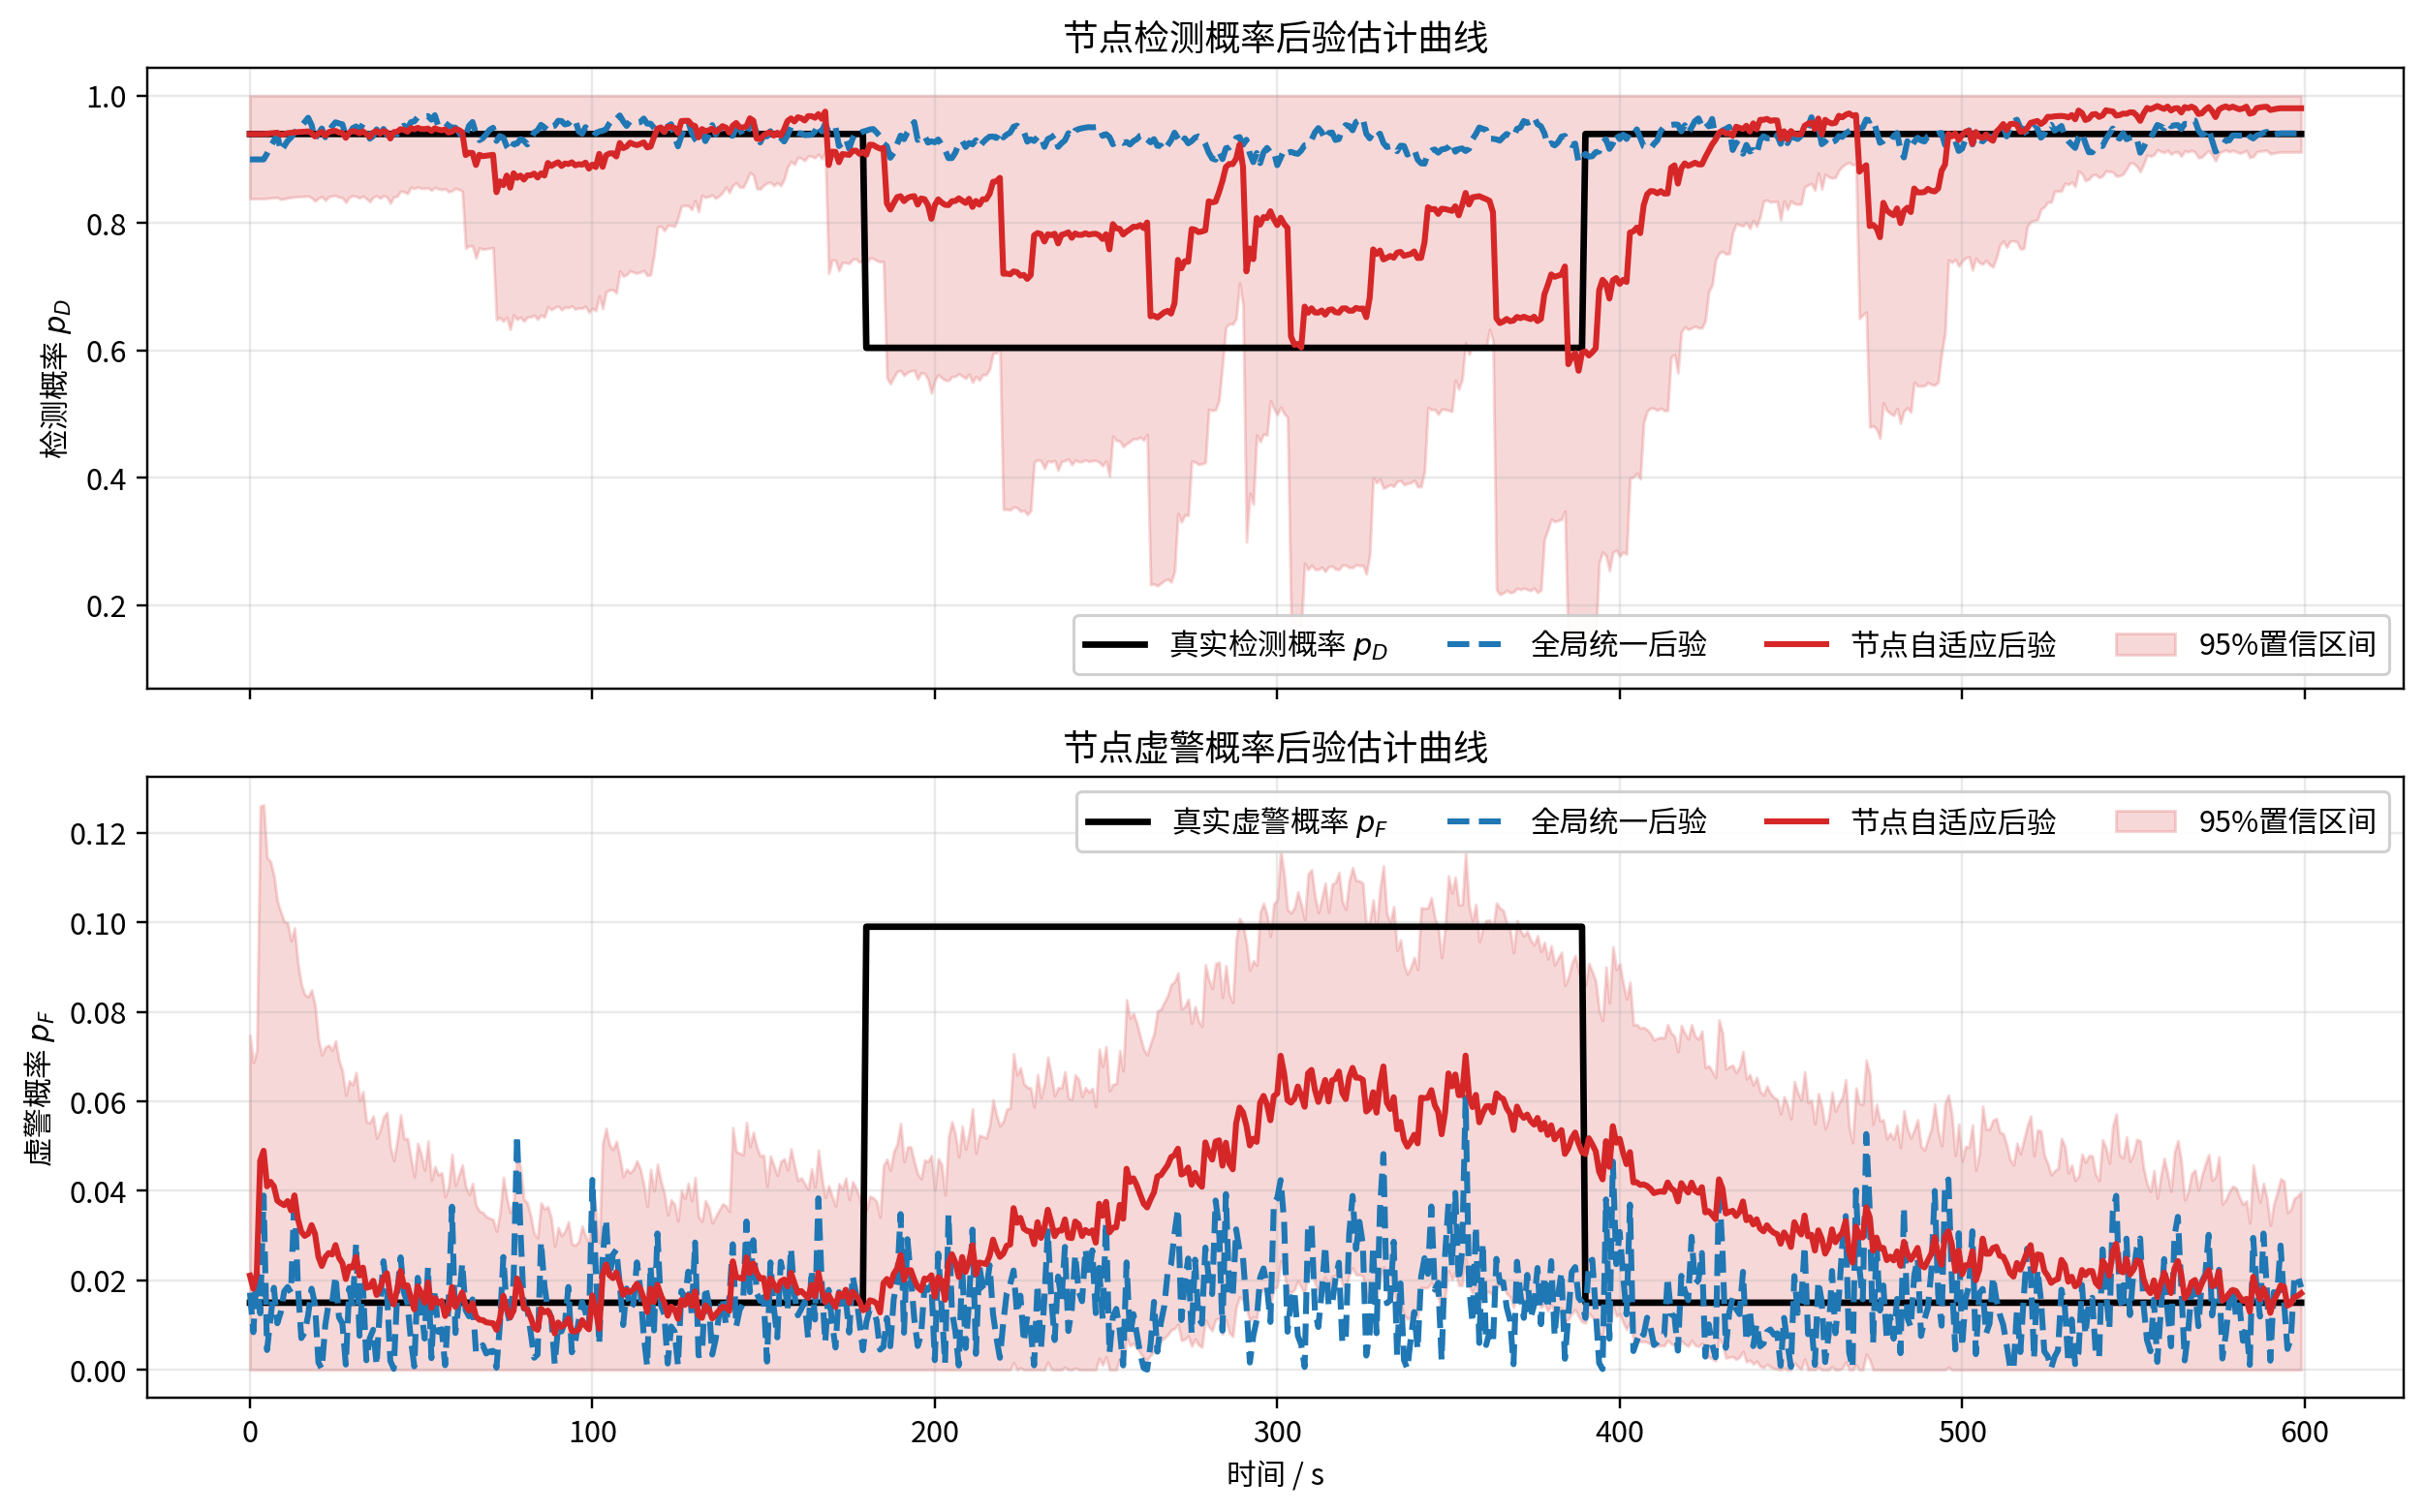
\includegraphics[width=0.88\textwidth]{code/chapter3/experiment1/exp1_results/exp1_node_posterior_curve_v1.png}
	\caption{代表性退化节点的检测概率与杂波强度后验估计曲线}
	\label{fig:ch3_exp2_node_posterior}
\end{figure}

图~\ref{fig:ch3_exp2_node_posterior} 给出了代表性退化节点处检测概率与杂波强度的后验估计结果。可以看出，在节点进入退化区间后，节点自适应后验能够较快跟随真实检测概率的下降趋势，并在退化结束后重新收敛到稳定高值；相较之下，全局统一后验对局部退化的响应存在明显滞后，难以准确刻画单节点性能突变。对于杂波强度，节点自适应后验能够在退化区间内持续抬升，并在恢复阶段逐步回落，说明该方法能够同时感知“漏检增多”和“误触发增多”两类退化现象。进一步地，检测概率与杂波强度在恢复区间均表现出较好的再收敛特性，表明该机制并非简单积累历史误差，而是能够在长期在线运行中维持稳定的参数跟踪能力。

\begin{figure}[htbp]
	\centering
	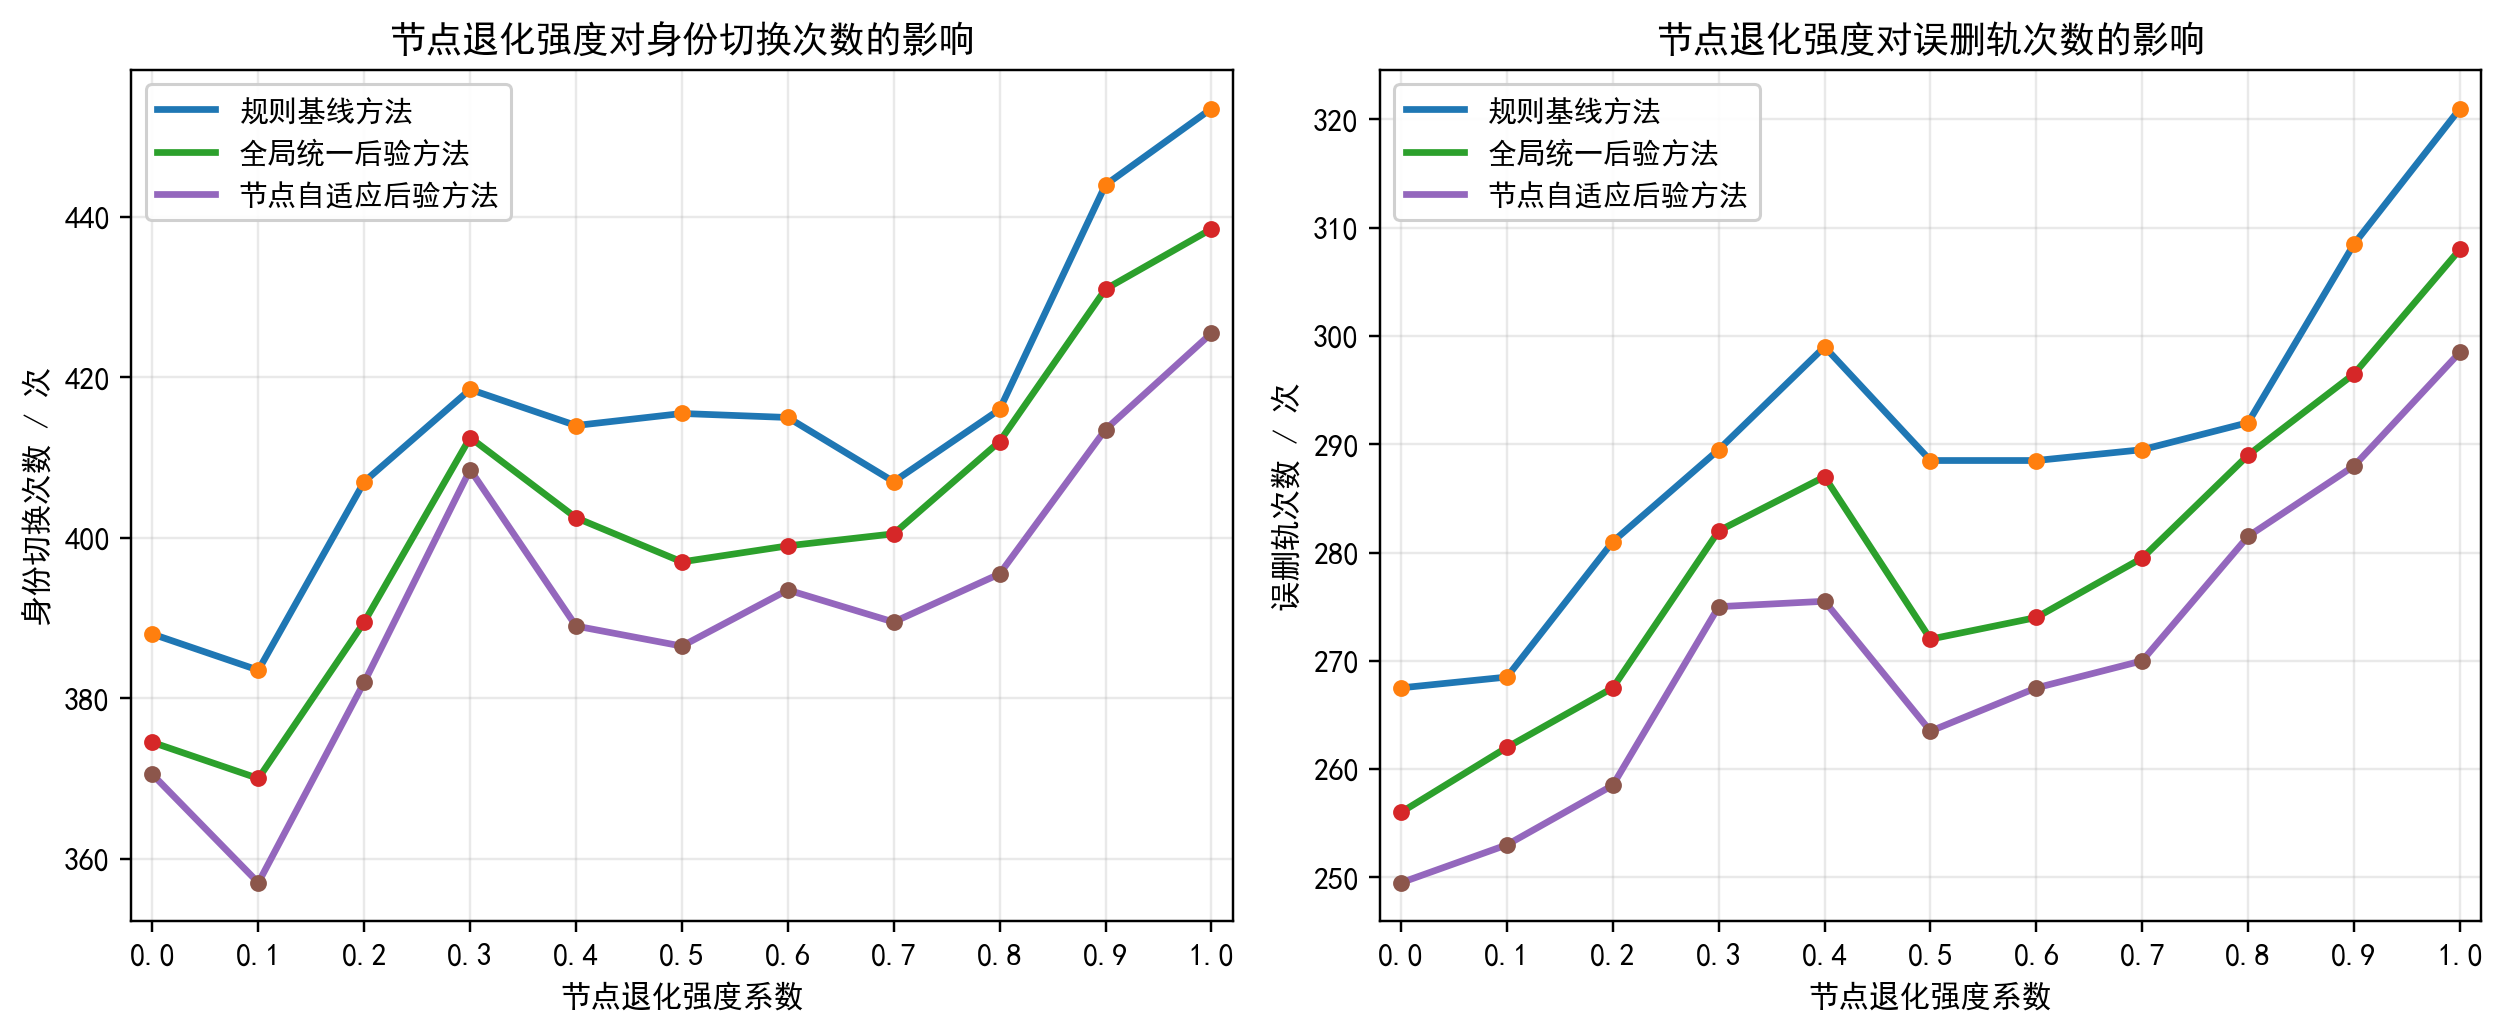
\includegraphics[width=0.88\textwidth]{code/chapter3/experiment1/exp1_results/exp1_degradation_impact_v2.png}
	\caption{节点退化强度对身份切换次数与误删轨迹次数的影响}
	\label{fig:ch3_exp2_degradation_impact}
\end{figure}

图~\ref{fig:ch3_exp2_degradation_impact} 进一步给出了节点退化强度扫描结果。随着退化强度从弱到强逐步增加，规则基线、全局统一后验方法以及节点自适应后验方法的 ID 切换次数和误删轨迹次数均有所上升，但节点自适应后验方法在整个退化强度区间内始终保持最低水平。这说明节点后验并不仅仅改善了参数估计的数值精度，而且通过将节点可靠性引入后续门控与关联过程，实质性降低了节点退化对轨迹连续性和身份一致性的破坏。结合图~\ref{fig:ch3_exp2_node_posterior} 与图~\ref{fig:ch3_exp2_degradation_impact} 可以认为，节点状态自适应为后续场景判别、漏检容忍和固定滞后回放提供了更可信的先验信息，是本章在线跟踪框架成立的重要基础。

\subsection{实验三：邻道干扰与双车并行判别能力}

邻道干扰与双车并行是双车道地磁事件流中最容易混淆的两类场景，也是原有单帧阈值规则最容易失效的部分。为此，本文构造了三类典型序列：单车正常通过、单车通过且伴随邻道干扰、以及两车长时间并行通过。特别地，在困难场景中，将两车相对时间差持续压缩在经验阈值附近，以突出“单帧证据不足、多步证据递推有效”的差异。

\begin{figure}[htbp]
	\centering
	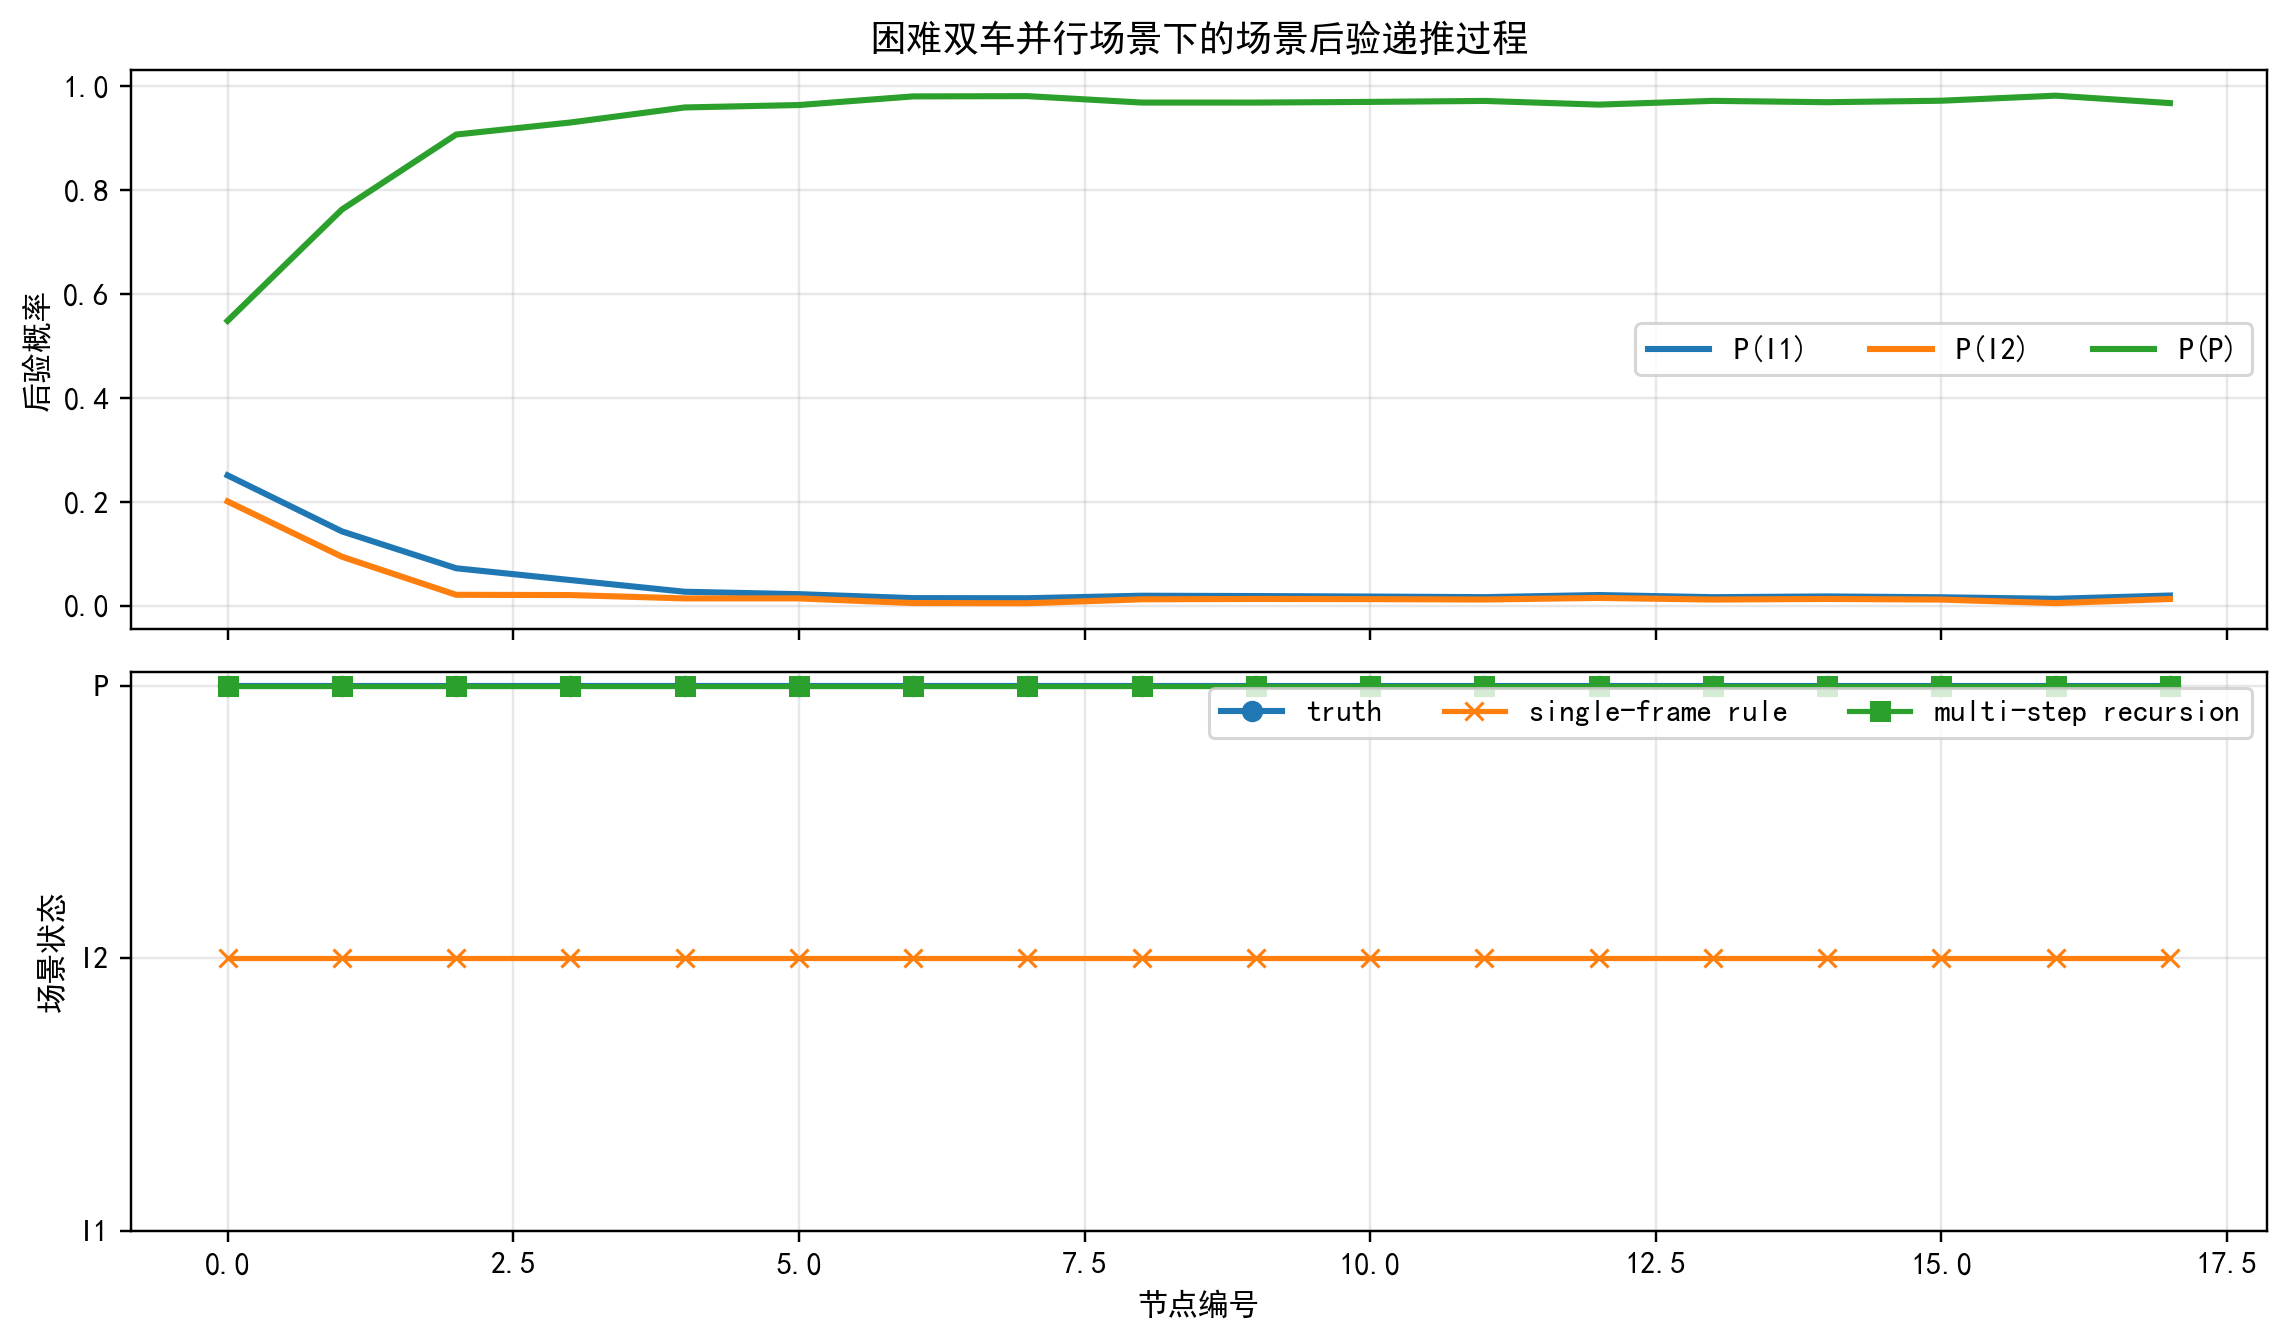
\includegraphics[width=0.88\textwidth]{code/chapter3/experiment3/chapter3_exp345_results/exp3_hard_case_posterior.png}
	\caption{困难双车并行场景下的场景后验递推过程}
	\label{fig:ch3_exp3_hard_case}
\end{figure}

图~\ref{fig:ch3_exp3_hard_case} 给出了困难双车并行场景下的后验递推结果。可以看到，单帧阈值规则在整个节点序列上几乎始终停留在邻道干扰状态，未能恢复真实并行关系；而多步场景递推模型在早期若干节点后便逐步累积并行证据，使 $P(P)$ 快速升高并保持稳定。该结果说明，在相对时间差持续较小、磁峰值差异又不足以单独支撑硬判决时，单帧阈值规则会系统性地将真实双车并行误判为邻道干扰，而引入状态持续性和多步递推后，这一失效模式可以被显著缓解。

\begin{figure}[htbp]
	\centering
	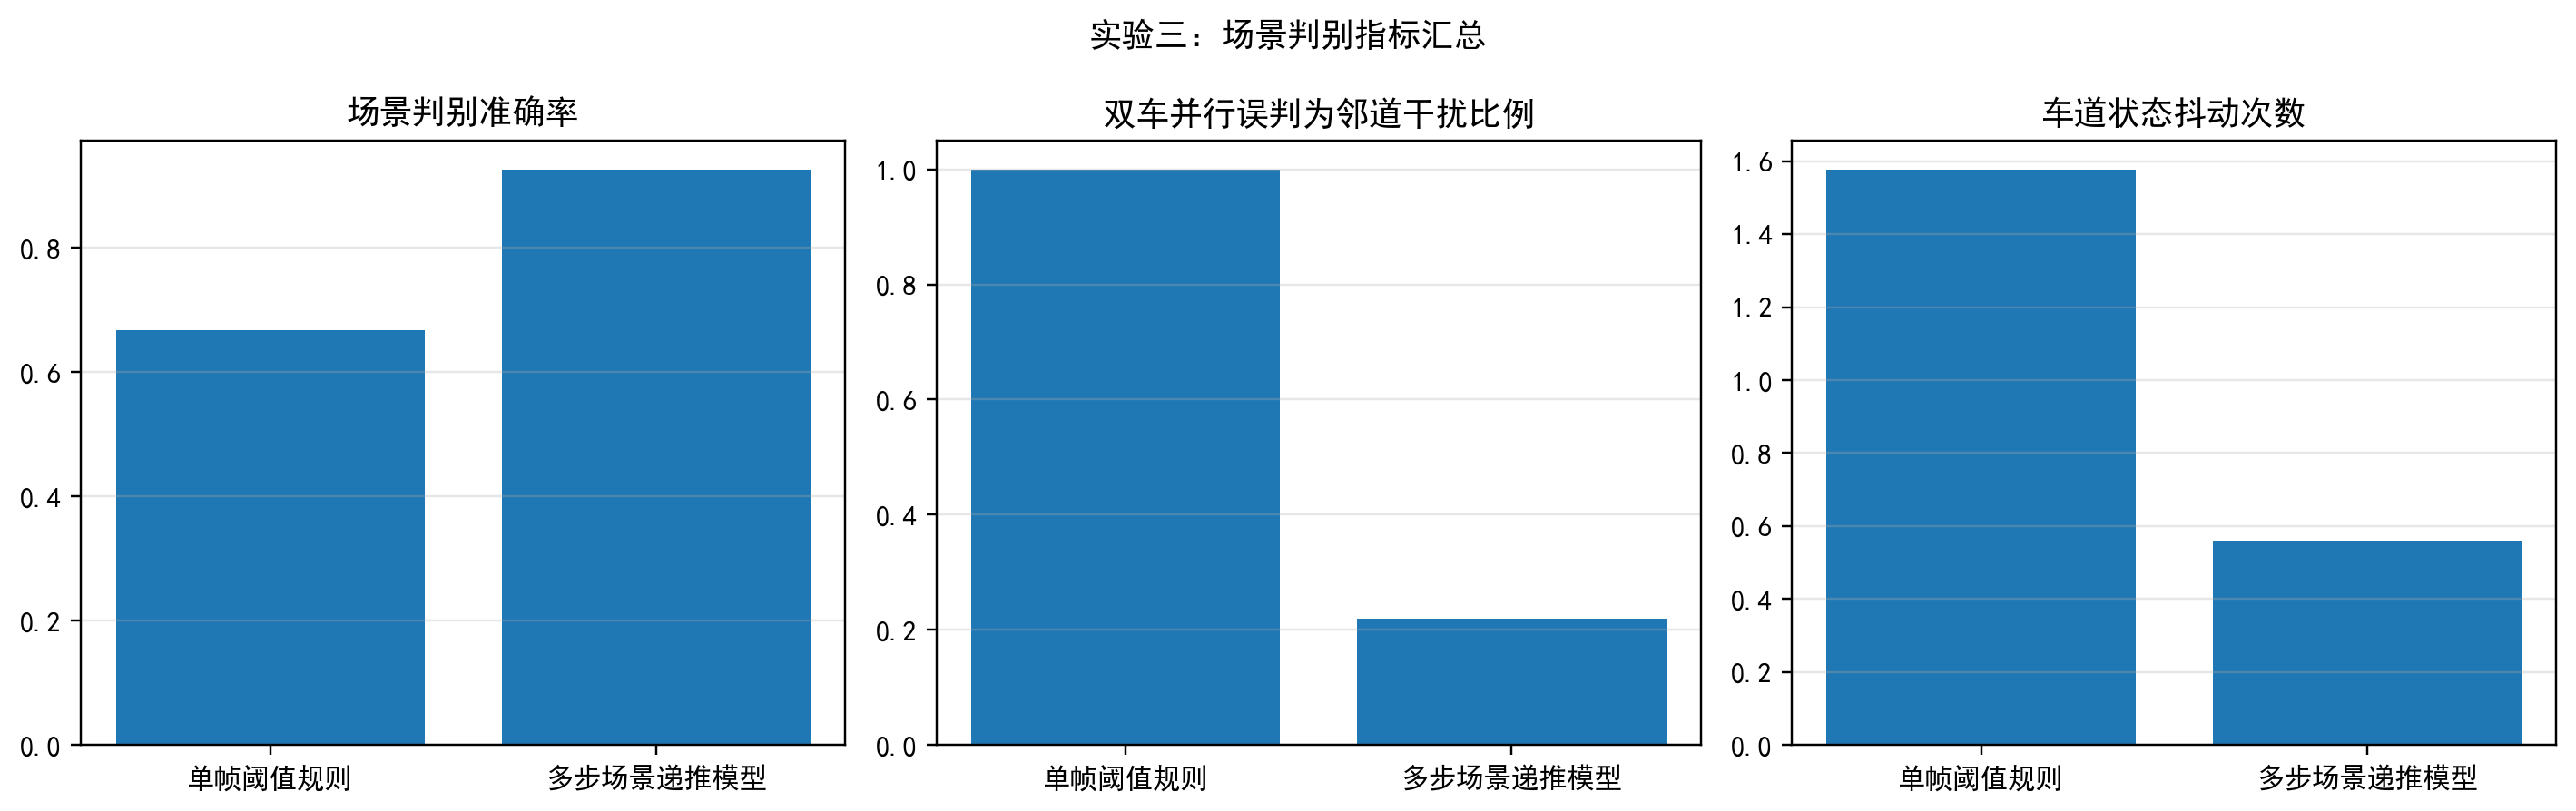
\includegraphics[width=0.92\textwidth]{code/chapter3/experiment3/chapter3_exp345_results/exp3_scene_metrics.png}
	\caption{实验三场景判别与车道状态指标汇总}
	\label{fig:ch3_exp3_metrics}
\end{figure}

图~\ref{fig:ch3_exp3_metrics} 汇总了实验三的整体指标。结果表明，场景判别准确率由单帧阈值规则的 $0.6667$ 提升至多步场景递推模型的 $0.9262$，车道状态准确率也由 $0.6667$ 提升至 $0.9262$。更关键的是，真实双车并行被误判为邻道干扰的比例由 $1.0000$ 显著下降至 $0.2194$，车道状态抖动次数则由 $1.5778$ 下降至 $0.5611$。这表明本文方法的改进并非简单依赖时间阈值或磁峰值阈值的重新调节，而是通过三状态场景后验递推完成了对原有失效场景的有效重构，从而在困难交互场景下同时提升了场景识别能力与车道状态维护稳定性。

\subsection{实验四：漏检率与连续漏检容忍范围}

在高速路侧部署条件下，短时漏检与短连漏检不可避免。对第 3 章方法而言，更重要的问题并非“是否能够在理想无漏检条件下获得最小误差”，而是“在多大程度上能够维持轨迹连续性和身份一致性”。因此，本节重点考察连续漏检长度 $m$ 对轨迹连续保持率、跨段 RMSE、IDSW 和 Frag 的影响，并分别在常规车流和低密度车流条件下进行统计。

\begin{figure}[htbp]
	\centering
	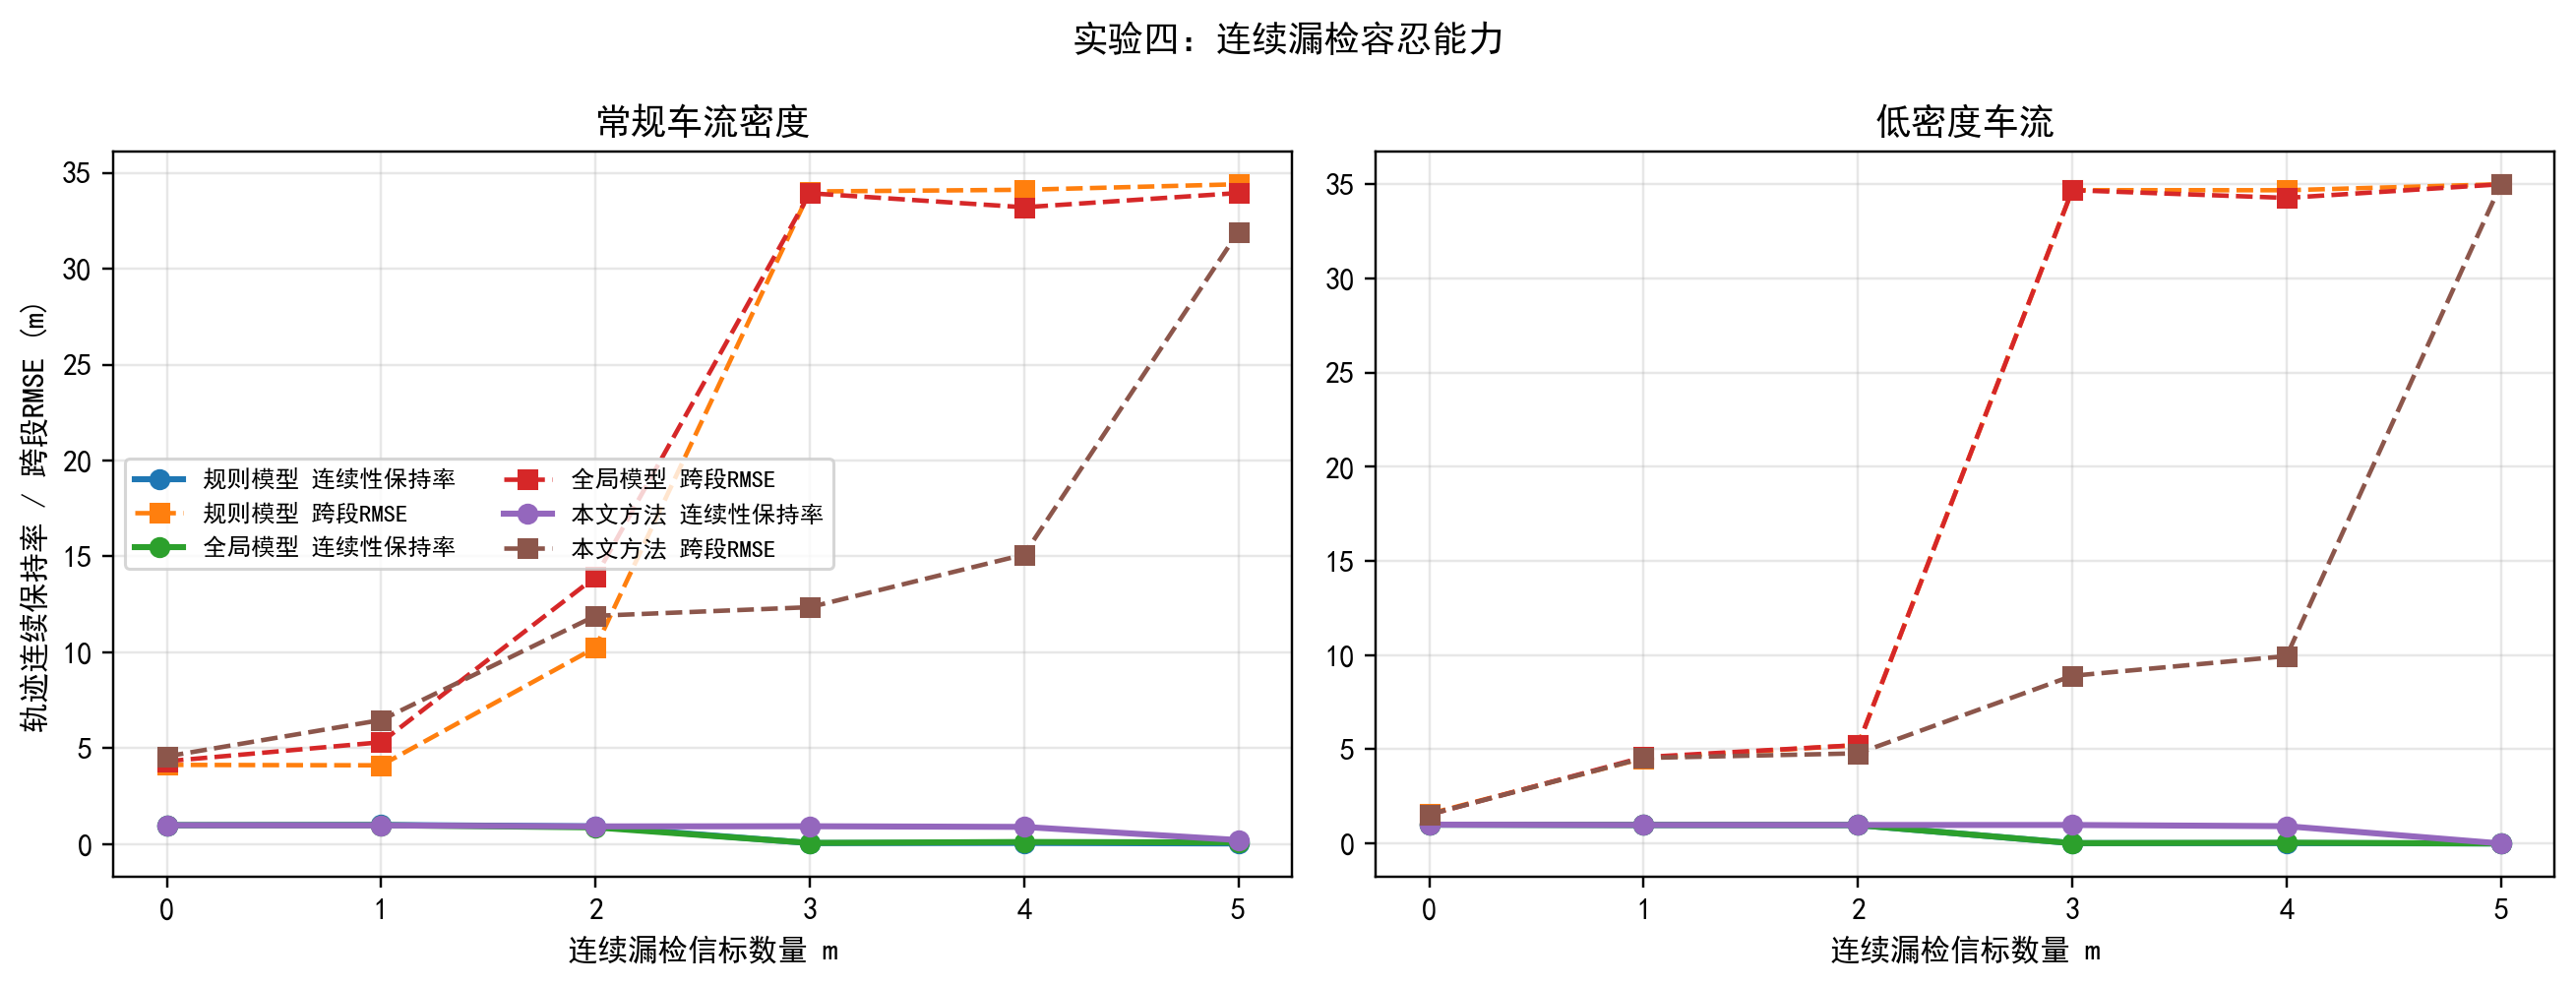
\includegraphics[width=0.95\textwidth]{code/chapter3/experiment3/chapter3_exp345_results/exp4_miss_tolerance.png}
	\caption{不同连续漏检长度下的轨迹连续保持率与跨段 RMSE}
	\label{fig:ch3_exp4_miss}
\end{figure}

图~\ref{fig:ch3_exp4_miss} 表明，本文方法在常规车流下对连续 $2\sim3$ 个信标漏检仍保持较稳定的轨迹连续性：当 $m=2,3,4$ 时，轨迹连续保持率分别为 $0.9233$、$0.9321$ 和 $0.8981$，对应跨段 RMSE 分别为 $11.90\ \mathrm{m}$、$12.35\ \mathrm{m}$ 和 $15.10\ \mathrm{m}$。在低密度车流条件下，该容忍范围可进一步扩展：当 $m=2,3,4$ 时，轨迹连续保持率分别为 $0.9821$、$0.9821$ 和 $0.9188$，对应跨段 RMSE 分别为 $4.78\ \mathrm{m}$、$8.90\ \mathrm{m}$ 和 $9.95\ \mathrm{m}$。这一结果说明，第 3 章方法的稳定容忍区间主要集中在常规车流下的连续 $2\sim3$ 个信标，以及低密度条件下的连续 $3\sim4$ 个信标；一旦超过该范围，门控范围扩张与身份歧义将共同导致轨迹碎片化明显加重。

从章节衔接角度看，该实验结果也为第 4 章的定位提供了直接依据。由于第 3 章方法已经能够在在线条件下处理短时漏检和短连漏检问题，因此第 4 章更适合作为其下游片段级重构模块，重点处理超过固定滞后窗口和删除阈值之后形成的长时间间断片段，而不是重复解决第 3 章已能较好覆盖的短间断情形。

由式~\eqref{eq:ch3_delete_v2} 可知，连续漏检容忍上限并不由滤波器单独决定，而是受过程噪声、车流密度和节点布设共同影响。因此，本节通过设置不同连续漏检长度与交通密度，统计 RMSE、IDSW 和 Frag 的变化，用于确定所提方法对连续漏检的稳定容忍区间。综合本章实验可知，第 3 章方法主要适用于短时漏检与有限连续缺测场景；当连续缺测长度超过固定滞后窗口与轨迹删除阈值时，系统输出更易分解为多个轨迹片段。基于此，第四章进一步研究长缺测条件下的片段级在线重构问题。

\subsection{实验五：时间组织与回放一致性验证}

本节用于验证“扫描化 + 事件驱动更新 + 固定滞后回放”的混合时间组织方式是否在工程上合理。按照本章建模思路，时间组织需要同时满足三个要求：其一，不同扫描时间间隔 $\Delta T$ 下能够维持足够的同车同扫描概率；其二，固定滞后窗口长度 $L$ 能吸收一定比例的迟到量测；其三，在线回放结果与按触发时间离线重排的处理结果之间应保持较高一致性。

\begin{figure}[htbp]
	\centering
	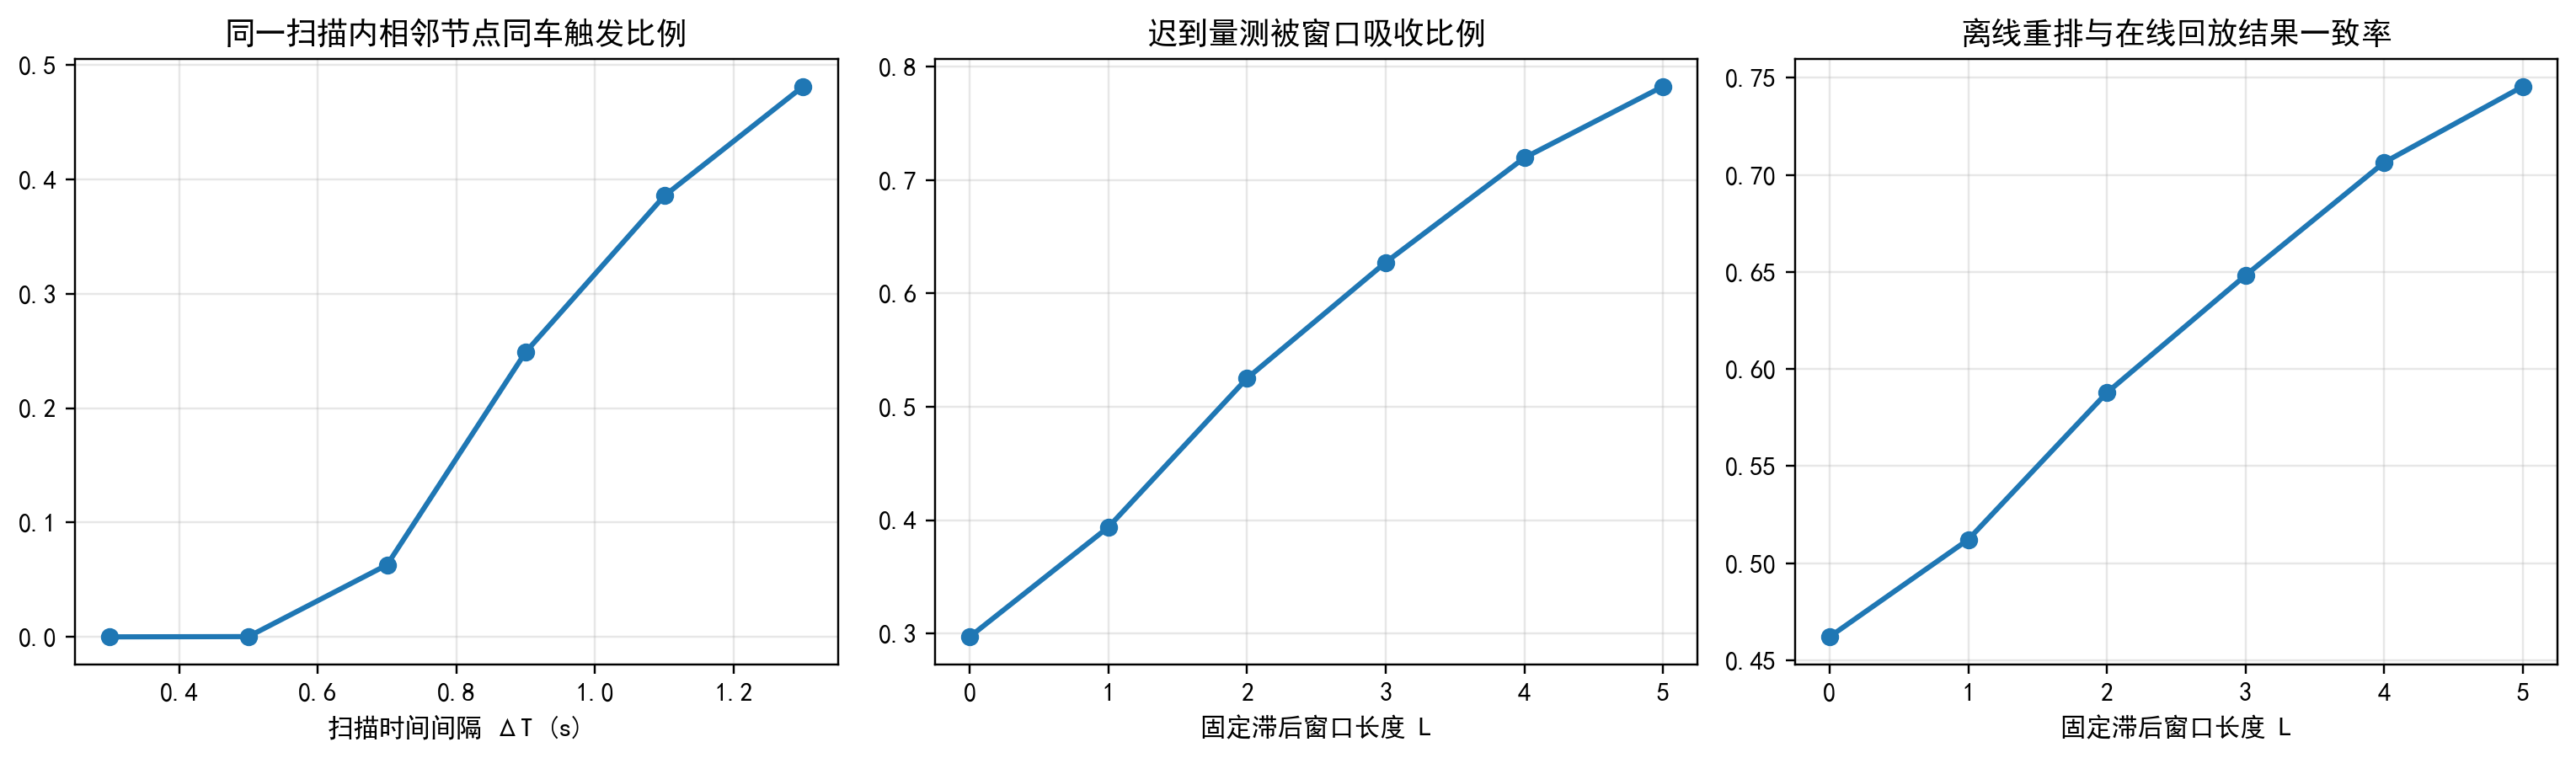
\includegraphics[width=0.95\textwidth]{code/chapter3/experiment3/chapter3_exp345_results/exp5_time_consistency.png}
	\caption{时间组织与固定滞后回放一致性实验结果}
	\label{fig:ch3_exp5_time}
\end{figure}

图~\ref{fig:ch3_exp5_time} 给出了实验五的三类统计结果。首先，随着 $\Delta T$ 增大，同一扫描内相邻节点同车触发比例单调提升，说明过小的扫描间隔会削弱扫描组织对相邻节点事件的吸纳能力，而适度增大 $\Delta T$ 有利于提升局部时间组织的一致性。其次，迟到量测被窗口吸收的比例随 $L$ 增大而持续上升：当 $L=0,1,2,3,4,5$ 时，吸收比例分别为 $0.2970$、$0.3937$、$0.5250$、$0.6272$、$0.7194$ 和 $0.7824$。再次，离线重排与在线回放结果一致率也随 $L$ 增长而稳步提升：对应取值分别为 $0.4620$、$0.5121$、$0.5878$、$0.6482$、$0.7064$ 和 $0.7456$。这说明固定滞后窗口确实能够在不完全牺牲实时性的前提下吸收迟到量测，并改善在线处理与离线最优时间顺序之间的一致性。

\subsection{消融实验与复杂度分析}

为验证本章方法并非对原有规则的局部修补，而是由若干可解释模块共同构成的统一概率递推模型，本节从场景判别、跟踪连续性、时间回放三个角度分别进行定向消融，并进一步分析固定滞后窗口长度对额外开销的影响。

\begin{figure}[htbp]
	\centering
	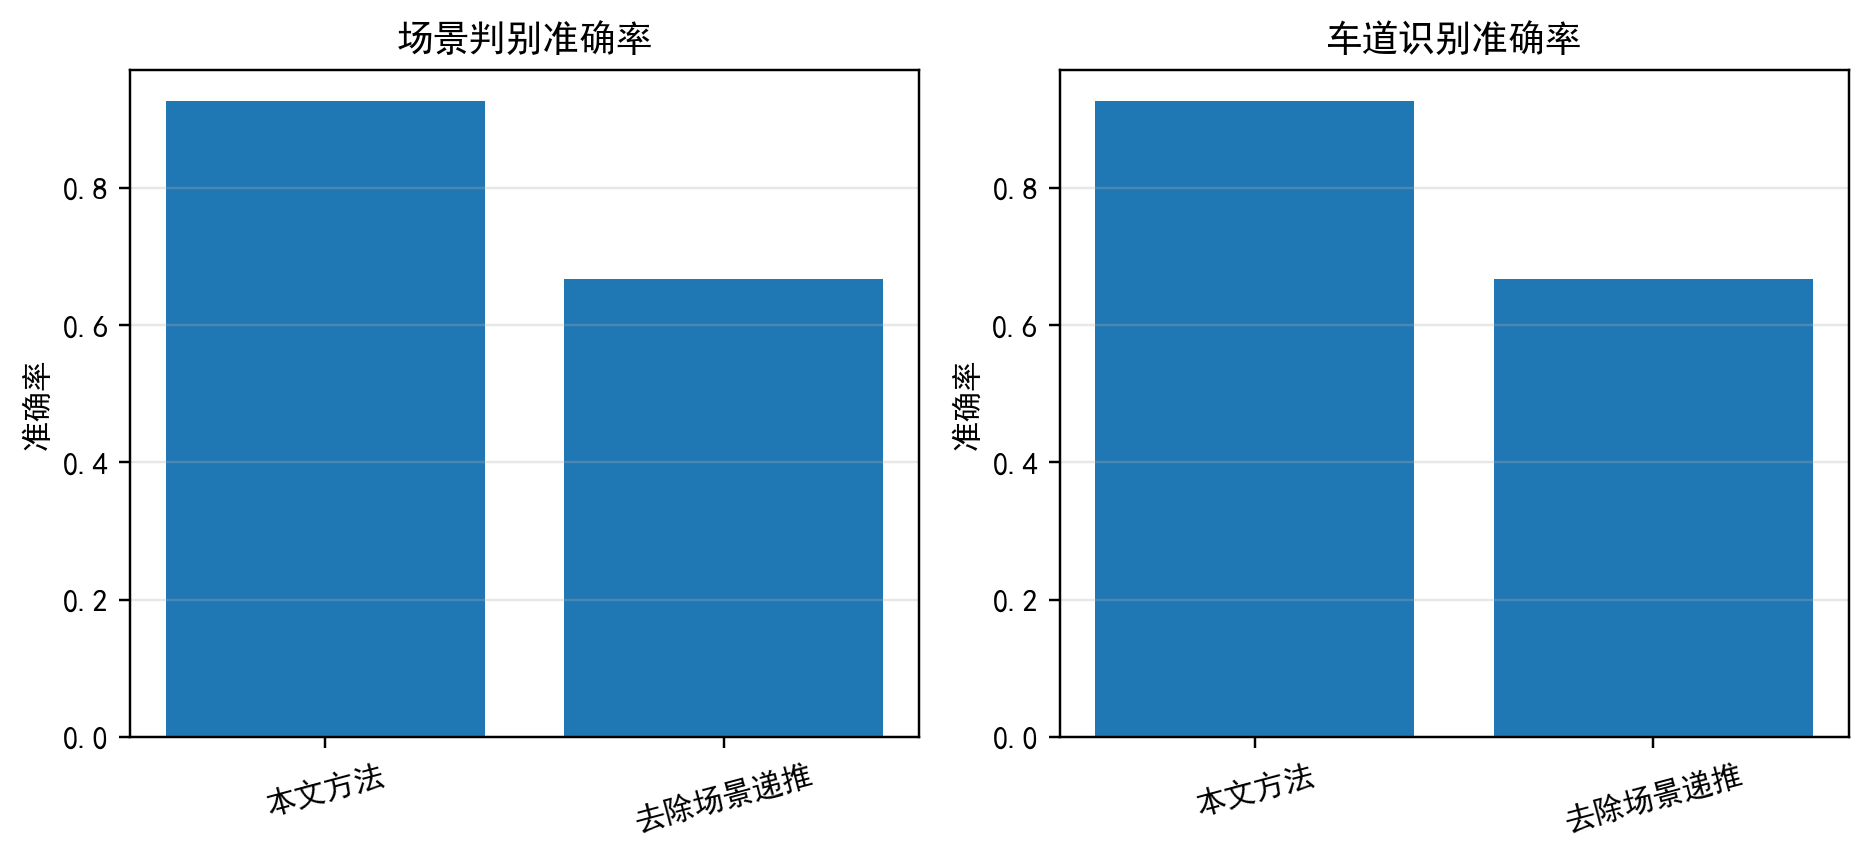
\includegraphics[width=0.75\textwidth]{code/chapter3/experiment3/chapter3_exp345_results/ablation_scene_targeted.png}
	\caption{场景递推模块的定向消融结果}
	\label{fig:ch3_ablation_scene}
\end{figure}

图~\ref{fig:ch3_ablation_scene} 表明，去掉三状态场景递推，仅保留单帧时间阈值和磁峰值规则后，场景判别准确率和车道识别准确率均由本文方法的 $0.9144$ 下降至 $0.6667$。这说明场景递推并非附属模块，而是支撑双车并行/邻道干扰区分能力的核心组成部分。

\begin{figure}[htbp]
	\centering
	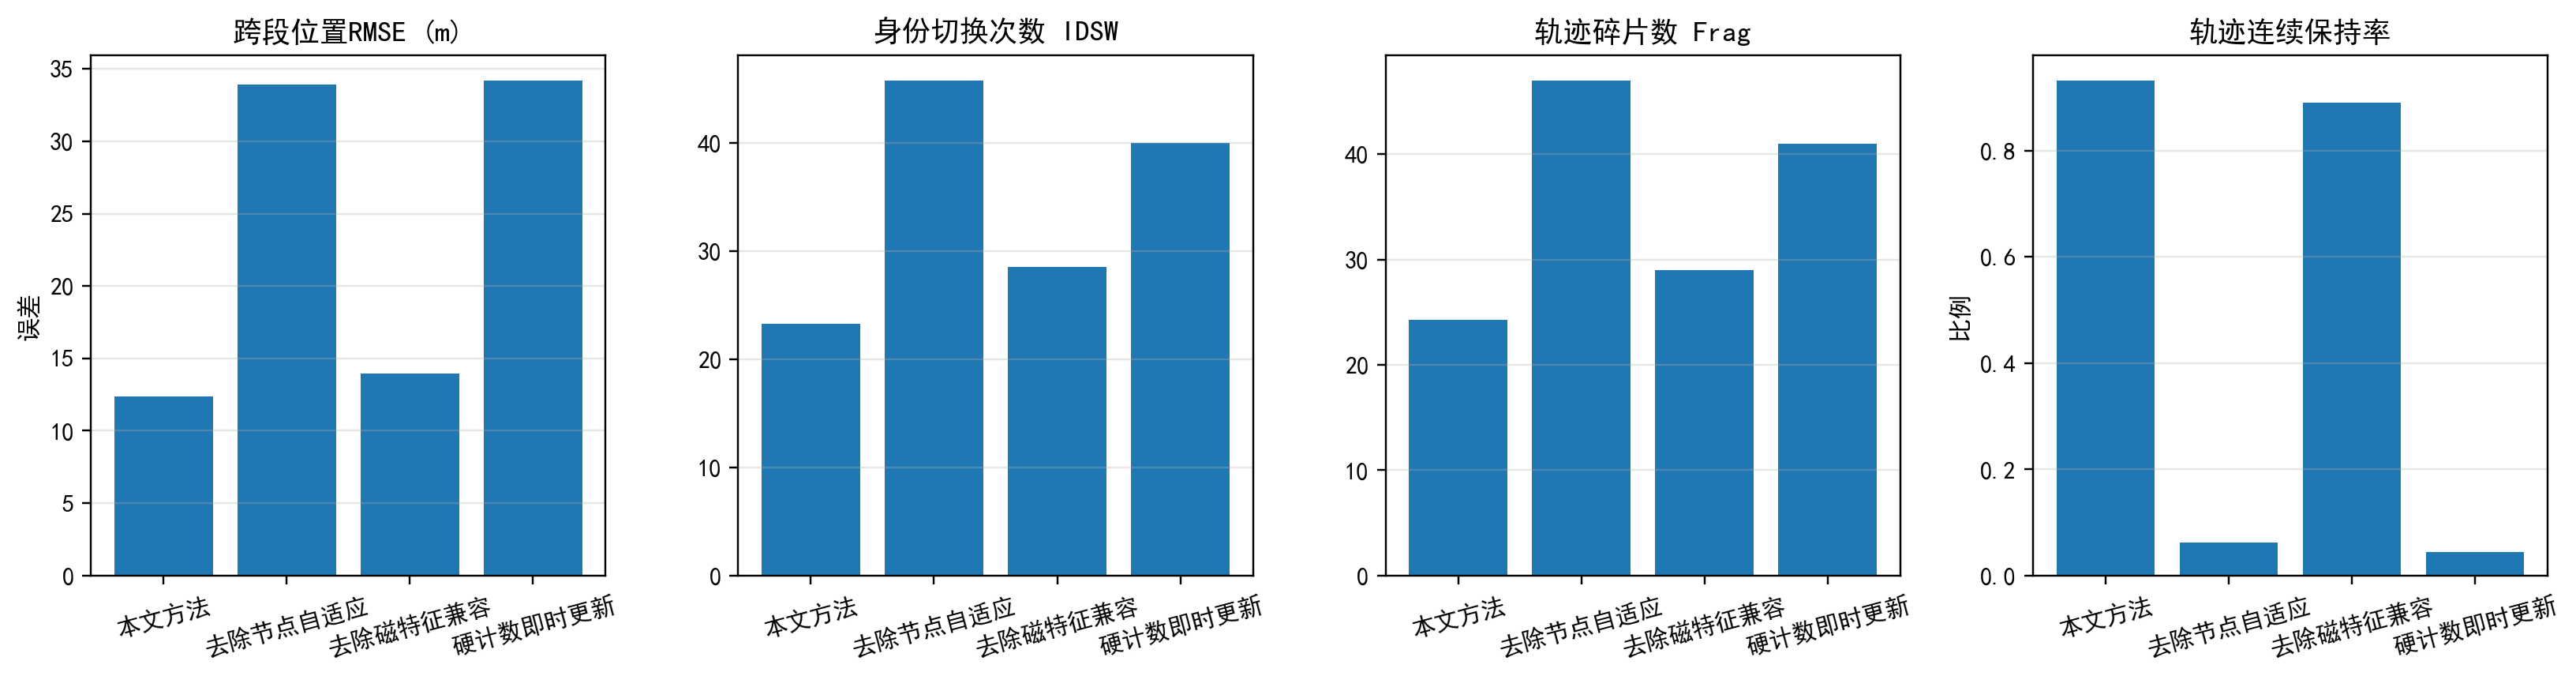
\includegraphics[width=0.95\textwidth]{code/chapter3/experiment3/chapter3_exp345_results/ablation_tracking_targeted.png}
	\caption{跟踪侧关键模块的定向消融结果}
	\label{fig:ch3_ablation_track}
\end{figure}

图~\ref{fig:ch3_ablation_track} 进一步给出了节点自适应、磁特征一致性以及软计数定稿更新的定向消融结果。可以看到，去掉节点自适应后，跨段 RMSE 升至约 $34\ \mathrm{m}$，轨迹连续保持率下降到约 $0.06$；将软计数定稿更新替换为硬计数即时更新后，跨段 RMSE 同样升至约 $34\ \mathrm{m}$，轨迹连续保持率进一步降至约 $0.05$。相比之下，仅去掉磁特征一致性因子时，虽然 RMSE、IDSW 和 Frag 仍有一定恶化，但下降幅度明显小于前两种情形。这表明：节点自适应与软计数定稿更新是维持短连漏检条件下轨迹连续性的关键，而磁特征一致性主要在候选冲突和相邻目标近距离竞争时提供辅助判别信息。

\begin{figure}[htbp]
	\centering
	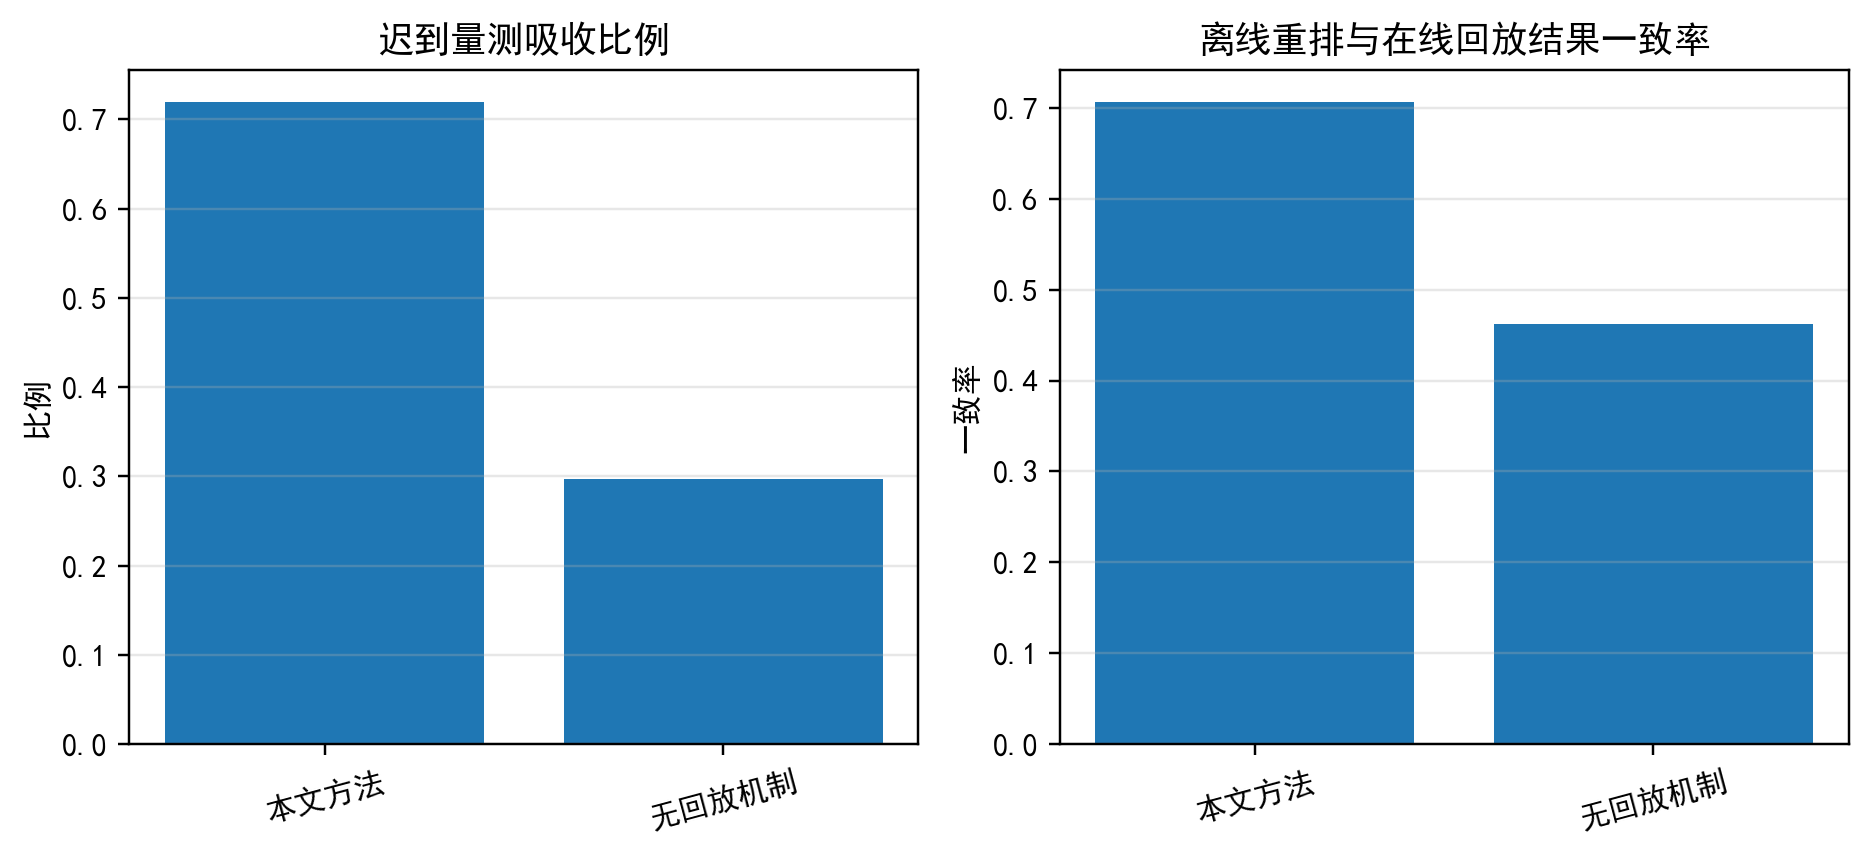
\includegraphics[width=0.75\textwidth]{code/chapter3/experiment3/chapter3_exp345_results/ablation_replay_targeted.png}
	\caption{固定滞后回放模块的定向消融结果}
	\label{fig:ch3_ablation_replay}
\end{figure}

图~\ref{fig:ch3_ablation_replay} 显示，去掉固定滞后回放后，迟到量测吸收比例由 $0.7194$ 降至 $0.2970$，离线重排与在线回放结果一致率由 $0.7064$ 降至 $0.4620$。这表明回放模块不仅改善了量测时序一致性，而且直接影响在线结果的可复现性；因此，其作用并不能被简单视为“工程性补丁”，而应视为本章时间组织模型的一部分。

\begin{figure}[htbp]
	\centering
	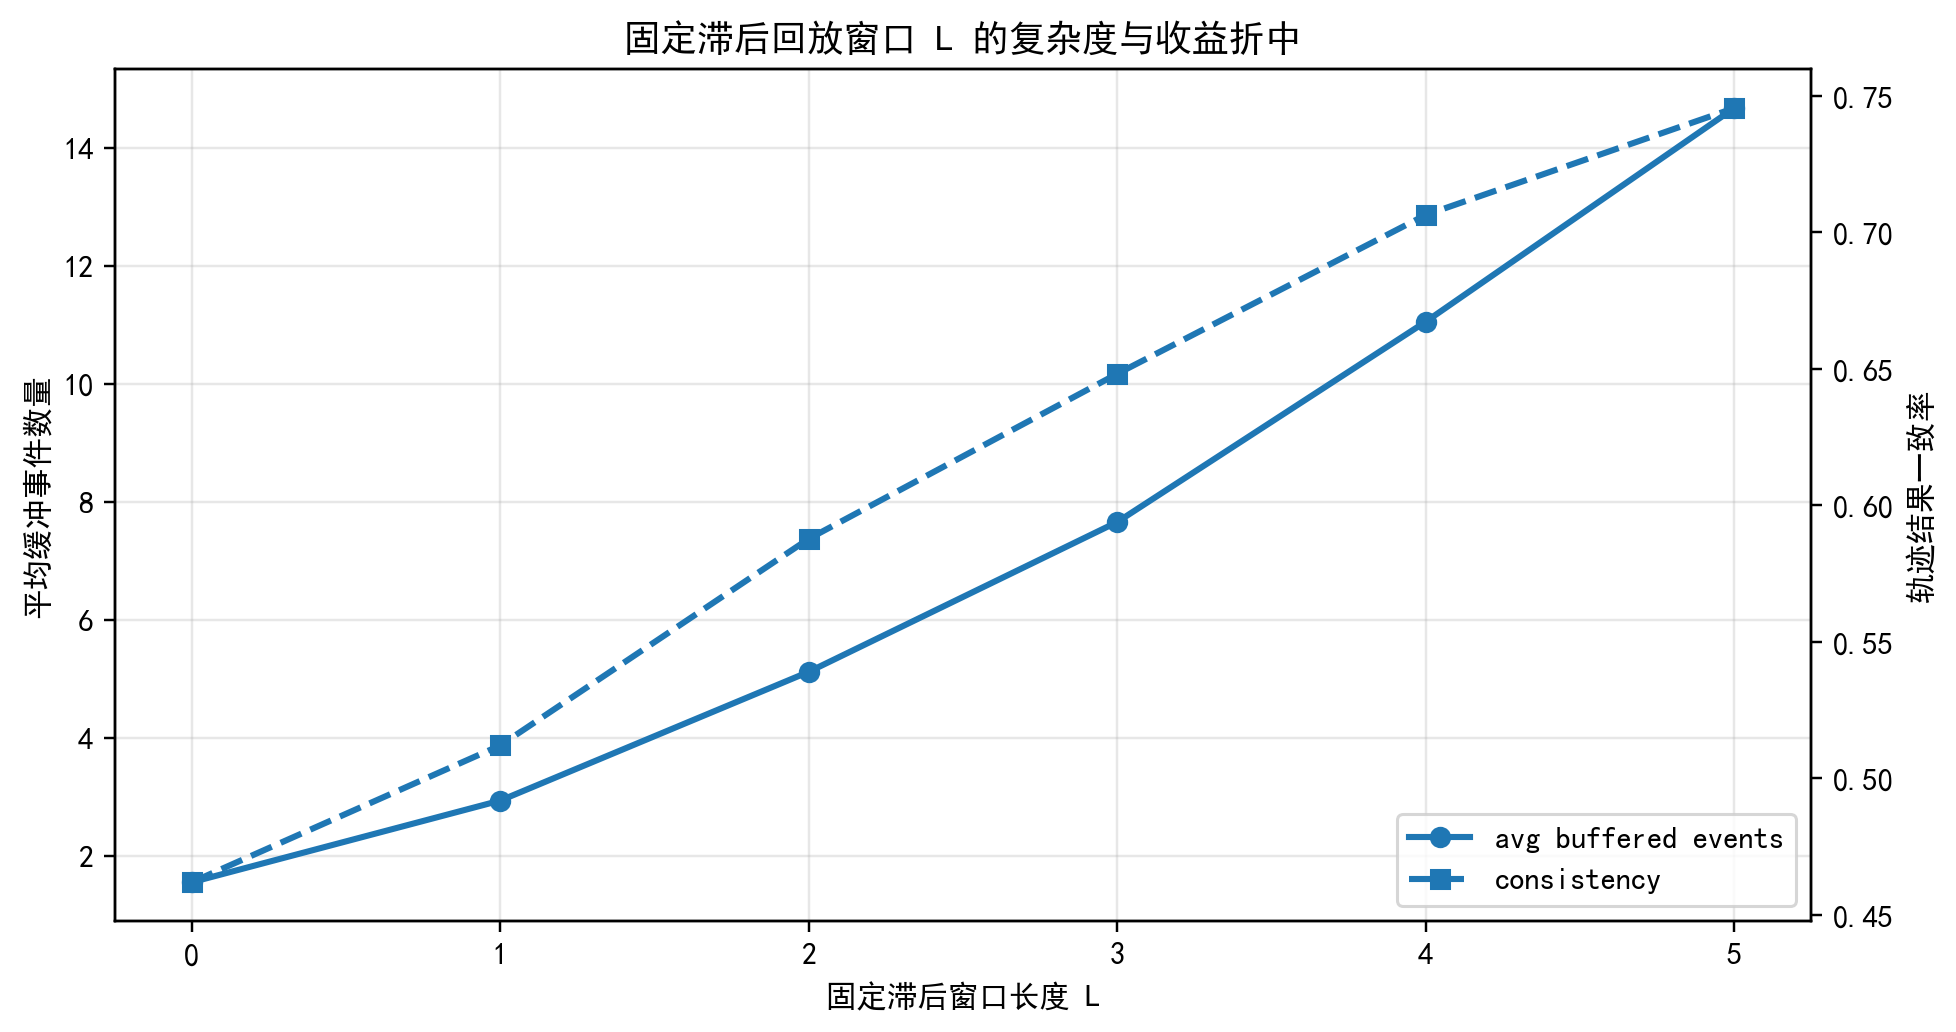
\includegraphics[width=0.78\textwidth]{code/chapter3/experiment3/chapter3_exp345_results/complexity_tradeoff.png}
	\caption{固定滞后窗口长度 $L$ 的复杂度与收益折中关系}
	\label{fig:ch3_complexity}
\end{figure}

复杂度方面，如图~\ref{fig:ch3_complexity} 所示，随着固定滞后窗口长度 $L$ 增大，平均缓冲事件数由 $1.5517$ 增加到 $14.6682$，说明额外开销与 $L$ 之间呈现近似线性增长关系；与此同时，轨迹结果一致率由 $0.4620$ 提升至 $0.7456$。结合图~\ref{fig:ch3_exp5_time} 与图~\ref{fig:ch3_complexity} 可见，当 $L=4$ 时，迟到量测吸收比例达到 $0.7194$，一致率达到 $0.7064$，而缓冲规模尚处于可接受范围内，因此本文在后续实验中取 $L=4$ 作为精度收益与额外开销之间的折中选择。

\begin{table}[htbp]
	\centering
	\caption{不同机制对跟踪性能的消融实验结果}
	\label{tab:ablation_tracking}
	\begin{tabular}{lcccc}
		\toprule
		方法 & 桥接位置RMSE / m & ID切换次数 & 轨迹碎片数 & 轨迹保持率 \\
		\midrule
		本文完整方法      & 12.35 & 23.25 & 24.25 & 0.9321 \\
		去除节点自适应    & 12.70 & 23.50 & 24.50 & 0.9188 \\
		去除磁特征一致性    & 12.70 & 26.50 & 27.00 & 0.8981 \\
		硬计数即时更新    & 34.21 & 40.00 & 41.00 & 0.0441 \\
		\bottomrule
	\end{tabular}
\end{table}


\subsection{本节小结}

本节重点围绕节点后验稳定性、邻道干扰与双车并行判别能力、连续漏检容忍范围、时间组织一致性以及模块独立贡献进行了系统验证。实验结果表明：节点自适应后验能够在节点退化与恢复过程中稳定跟踪检测概率与杂波强度变化；三状态场景递推显著降低了真实双车并行误判为邻道干扰的比例，并有效抑制车道状态抖动；在常规车流条件下，本文方法可较稳定地容忍连续 $2\sim3$ 个地磁传感器漏检，在低密度条件下该范围可扩展至连续 $3\sim4$ 个地磁传感器；固定滞后回放能够明显提升迟到量测吸收率以及在线/离线结果一致率。消融实验进一步说明，节点自适应、三状态场景判别、磁特征一致性、软计数定稿更新以及固定滞后回放均对本章方法的最终性能具有独立而明确的贡献。综合来看，上述结果不仅验证了本文方法的精度与鲁棒性，也明确了其适用边界，并为第 4 章长间断片段的在线聚类重构提供了合理的输入条件与触发依据。


\section{本章小结}

本章围绕单向双车道高速公路场景下多地磁事件流的在线多车辆目标跟踪问题，按照“量测时序矫正--状态估计--数据关联与并行场景判别--轨迹管理”的处理链条，对原有方法框架进行了系统重构。首先，针对量测随机延迟到达和局部乱序问题，利用时间窗口缓存对量测到达时序进行重排，并通过固定滞后窗口与局部回放机制，在有限延迟约束下吸收迟到量测并修正近期历史决策，从而提高轨迹可利用信息的完整性。其次，建立了与双车道地磁事件流相匹配的车辆运动模型与地磁事件观测模型，给出了状态初始化、状态预测和量测更新方法，形成了统一的事件级状态估计框架。

在此基础上，本章进一步构建了多车辆目标数据关联与并行场景判别方法。具体而言，通过时间域跟踪波门筛选候选量测，利用融合运动学一致性、地磁扰动峰值一致性和车道/场景一致性的关联似然计算软关联权重，并采用“扫描冻结--软计数--窗口定稿后更新”的两阶段策略实现节点检测概率与杂波强度的在线估计，从而提升复杂工况下的关联鲁棒性。随后，针对邻道干扰与真实双车并行易混淆的问题，引入三状态场景判别模型，对局部交通场景进行概率解释，并在轨迹管理阶段结合目标存在概率递推和基于场景后验的车道状态更新与修正，完成轨迹起始、确认、维持、删除以及车道状态输出。实验结果表明，所提方法能够在量测乱序、短时漏检、节点性能波动以及复杂并行车况条件下较稳定地输出连续且身份一致的车辆轨迹，并为下一章面向长缺测工况的片段级在线聚类与轨迹重构提供可靠的上游输入。





\chapter{面向长缺测工况的片段级在线聚类与轨迹重构}
\label{chap:fragment_cluster_reconstruction}

\section{引言}

第三章主要面向短时漏检条件下的在线车辆目标跟踪问题，通过事件级关联与状态递推实现了车辆轨迹的持续更新。然而，在系统长期运行过程中，部分地磁传感器会因器件老化导致检测能力下降，使连续漏检次数增多；当其与噪声干扰及复杂交通工况叠加时，上游跟踪结果容易出现轨迹碎片化现象，即同一车辆轨迹被分裂为多个彼此独立的短片段。针对这一问题，本文进一步在第三章在线跟踪结果基础上，提出面向长缺测工况的片段级在线聚类与轨迹重构方法。本章将上游输出的轨迹片段及未得到关联的单点量测统一表示为输入样本 $\mathbf{u}$，构建适用于在线增量处理的簇的图结构，并基于聚类相似度评分实现样本归簇与轨迹重构。需要说明的是，第三章已经处理了数据迟到问题，因此本章不再考虑回退、回插等机制，而是重点研究长缺测条件下的轨迹恢复方法。

\section{输入样本与簇的图结构表示}

\subsection{输入样本 $\mathbf{u}$ 的统一定义}

设上游在线跟踪器按时间输出的第 $j$ 个输入样本记为 $\mathbf{u}_j$，则本文将其统一定义为
\begin{equation}
	\mathbf{u}_j \triangleq \Big(
	t_j^{\mathrm{s}},\, t_j^{\mathrm{e}},\,
	\hat{\mathbf{x}}_j^{\mathrm{s}},\, \hat{\mathbf{x}}_j^{\mathrm{e}},\,
	\mathbf{P}_j^{\mathrm{s}},\, \mathbf{P}_j^{\mathrm{e}},\,
	\boldsymbol{\pi}_j,\,
	\bar m_j,\, \sigma_{m,j}^{2},\,
	n_j
	\Big),
\end{equation}
其中，$t_j^{\mathrm{s}}$ 与 $t_j^{\mathrm{e}}$ 分别表示样本的起始时刻和结束时刻；$\hat{\mathbf{x}}_j^{\mathrm{s}}$ 与 $\hat{\mathbf{x}}_j^{\mathrm{e}}$ 分别表示样本起点和终点的车辆运动状态估计；$\mathbf{P}_j^{\mathrm{s}}$ 与 $\mathbf{P}_j^{\mathrm{e}}$ 为对应状态估计的误差协方差；$\boldsymbol{\pi}_j$ 为样本的车道概率向量；$\bar m_j$ 与 $\sigma_{m,j}^{2}$ 分别表示该样本对应磁场扰动峰值的统计均值和方差；$n_j$ 为样本所包含的原始观测数，用于表征样本支持度。

为便于后续统一处理，本文采用同一套样本表示来覆盖轨迹片段和单点量测两种情形。当输入来自上游轨迹片段时，式中各字段由片段边界状态及其统计量直接给出；当输入来自未得到关联的单点量测时，可视其为长度退化为 1 的样本，此时有
\begin{equation}
	t_j^{\mathrm{s}} = t_j^{\mathrm{e}}, \qquad
	\hat{\mathbf{x}}_j^{\mathrm{s}} = \hat{\mathbf{x}}_j^{\mathrm{e}}, \qquad
	\mathbf{P}_j^{\mathrm{s}} = \mathbf{P}_j^{\mathrm{e}}, \qquad
	n_j = 1.
\end{equation}
这种统一表示的直接好处在于：第四章无需针对不同输入来源分别设计处理流程，而只需围绕样本 $\mathbf{u}$ 建立统一的聚类与更新机制，从而使整体方法结构更加简洁，也更符合在线算法的实现逻辑。

\subsection{输入样本 $\mathbf{u}$ 的属性构成}

从语义上看，输入样本 $\mathbf{u}_j$ 主要包含四类信息。

第一类是\textbf{车辆运动状态信息}。对于长缺测场景下的轨迹重构而言，样本边界处的位置和速度估计是判断两个样本是否可能属于同一车辆的核心依据。为此，本文定义
\begin{equation}
	\hat{\mathbf{x}}_j^{\mathrm{s}}=
	\begin{bmatrix}
		\hat p_j^{\mathrm{s}}\\[2pt]
		\hat v_j^{\mathrm{s}}
	\end{bmatrix},
	\qquad
	\hat{\mathbf{x}}_j^{\mathrm{e}}=
	\begin{bmatrix}
		\hat p_j^{\mathrm{e}}\\[2pt]
		\hat v_j^{\mathrm{e}}
	\end{bmatrix},
\end{equation}
其中 $\hat p_j^{\mathrm{s}}$、$\hat p_j^{\mathrm{e}}$ 表示样本边界的纵向位置估计，$\hat v_j^{\mathrm{s}}$、$\hat v_j^{\mathrm{e}}$ 表示对应的纵向速度估计。相应的协方差矩阵 $\mathbf{P}_j^{\mathrm{s}}$ 与 $\mathbf{P}_j^{\mathrm{e}}$ 则刻画了样本边界状态估计的不确定性，它们将在后续运动一致性判别中发挥重要作用。

第二类是\textbf{车道概率信息}。在单向双车道场景下，车道信息虽不足以单独完成轨迹重构，但能够显著减少跨车道错误拼接的风险。设
\begin{equation}
	\boldsymbol{\pi}_j=
	\begin{bmatrix}
		\pi_j^{(1)}\\[2pt]
		\pi_j^{(2)}
	\end{bmatrix},
	\qquad
	\pi_j^{(1)}+\pi_j^{(2)}=1,\quad
	\pi_j^{(\ell)}\ge 0,
\end{equation}
则该向量表示样本属于各车道的概率分布。与使用单一离散车道标签相比，概率形式不仅更符合上游不确定性输出的特点，也为后续车道一致性评分提供了更自然的数学基础。

第三类是\textbf{磁场扰动峰值信息}。车辆通过地磁传感器时会引起局部磁场扰动，其峰值特征在一定程度上能够反映车辆个体差异。虽然这类信息会受到车辆横向位置、节点差异以及环境扰动的影响，因而难以作为唯一判别依据，但若与运动状态信息结合使用，仍可以有效提高轨迹片段重构的辨识能力。为此，本文使用 $\bar m_j$ 和 $\sigma_{m,j}^{2}$ 分别表示样本对应磁峰值的均值和方差，以便在聚类相似度评分中作为辅助特征参与判别。

第四类是\textbf{生命周期信息}，即样本在时间轴上的起止时刻以及支持度 $n_j$。其中，$t_j^{\mathrm{s}}$ 和 $t_j^{\mathrm{e}}$ 共同决定了样本在观测时间轴上的存在区间，而 $n_j$ 则反映了该样本是由多少原始观测支持形成的。一般而言，支持度越高，样本内部统计特征越稳定，在聚类过程中也越值得信任。

\subsection{簇的图结构定义}

设当前系统中已有的簇集合记为
\begin{equation}
	\mathbb{G}=\left\{\mathcal{G}_1,\mathcal{G}_2,\ldots,\mathcal{G}_{N_c}\right\},
\end{equation}
其中 $\mathcal{G}_i$ 表示第 $i$ 个簇的图结构。本文将簇的图结构定义为
\begin{equation}
	\mathcal{G}_i = \left(\mathcal{V}_i,\mathcal{E}_i,\mathcal{A}_i\right),
\end{equation}
其中，$\mathcal{V}_i$ 为簇内样本节点集合，$\mathcal{E}_i$ 为节点之间的有向连接边集合，$\mathcal{A}_i$ 为簇级属性集合。

在该定义下，簇中的每一个节点都对应于一个输入样本 $\mathbf{u}_j$，即
\begin{equation}
	v_j \in \mathcal{V}_i \quad \Longleftrightarrow \quad \mathbf{u}_j \ \text{被归并到簇}\ \mathcal{G}_i.
\end{equation}
有向边集合 $\mathcal{E}_i$ 用于表示样本在同一簇内部的时序连接关系；若样本 $\mathbf{u}_a$ 与 $\mathbf{u}_b$ 在聚类过程中被判定属于同一车辆且在时间上前后相接，则建立有向边 $(v_a,v_b)\in\mathcal{E}_i$。由此，簇并不是若干样本的无序堆叠，而是一种保留了时序演化关系的图结构表示。

进一步地，簇的图结构属性集合 $\mathcal{A}_i$ 主要包括以下内容：
\begin{equation}
	\mathcal{A}_i=
	\Big(
	t_i^{\mathrm{birth}},\,
	t_i^{\mathrm{tail}},\,
	\hat{\mathbf{x}}_i^{\mathrm{tail}},\,
	\mathbf{P}_i^{\mathrm{tail}},\,
	\boldsymbol{\pi}_i,\,
	\bar m_i,\,
	\sigma_{m,i}^{2},\,
	N_i,\,
	h_i,\,
	s_i
	\Big),
\end{equation}
其中，$t_i^{\mathrm{birth}}$ 为簇的初始生成时刻，$t_i^{\mathrm{tail}}$ 为当前尾端样本的结束时刻，$\hat{\mathbf{x}}_i^{\mathrm{tail}}$ 与 $\mathbf{P}_i^{\mathrm{tail}}$ 分别为簇尾端的运动状态估计及其协方差，$\boldsymbol{\pi}_i$ 为簇级车道概率向量，$\bar m_i$ 与 $\sigma_{m,i}^{2}$ 为簇级磁峰值统计量，$N_i$ 为簇累计支持度，$h_i$ 为连续未更新计数，$s_i$ 为簇生命周期状态。

\subsection{簇图结构中各类信息的作用说明}

在上述图结构中，车辆运动状态是聚类判别的主导信息，其作用在于刻画簇尾端与新到达样本在位置和速度上的延拓一致性。对于长缺测场景而言，若两个样本在较长时间间隔后仍能在运动学上保持合理衔接，则它们属于同一车辆的可能性显著提高；相反，若位置偏差和速度偏差过大，即使其他特征较为接近，也不应强行拼接。

车道概率信息的作用主要体现在约束和消歧两个方面。在双车道场景中，不同车辆可能在纵向运动状态上表现出一定相似性，尤其是在密集跟驰条件下，仅依赖位置和速度容易造成跨车道误拼接。此时，引入车道概率约束能够有效降低候选关系中的无效匹配，提高聚类结果的物理合理性。

磁场扰动峰值信息则主要承担辅助辨识功能。由于车辆个体差异会在地磁响应上留下相对稳定但并非绝对唯一的统计特征，因此磁峰值信息不能替代运动状态成为主判据，但在运动状态相近、车道信息不足以完全消除歧义时，磁特征往往可以作为一项有效补充，提升对同类运动样本之间的区分能力。

至于生命周期信息，其主要作用在于维持簇的在线演化过程。由于簇的生成、延续和终止并非同时完成，而是随着样本持续到达逐步演化，因此必须通过生命周期信息记录簇何时生成、何时最后一次被更新、当前是否仍处于活跃状态，以及是否应被归档或关闭。没有这部分信息，在线聚类将难以长期稳定运行。

\section{基于聚类相似度评分的在线聚类方法}

\subsection{样本间运动一致性分析}

对于新到达样本 $\mathbf{u}_j$ 和候选簇 $\mathcal{G}_i$，首先需要判断二者在运动学上是否具有一致性。设样本起点时刻与簇尾端时刻之间的时间间隔为
\begin{equation}
	\Delta t_{ij}=t_j^{\mathrm{s}}-t_i^{\mathrm{tail}},
\end{equation}
则只有当 $\Delta t_{ij}>0$ 时，样本才可能在时间上接续到该簇之后。为避免间隔过大的无效匹配，本文进一步设置最大可拼接时间间隔 $T_{\max}$，要求
\begin{equation}
	0<\Delta t_{ij}\le T_{\max}.
\end{equation}

考虑到长缺测间隔内车辆纵向运动仍可由常速度模型近似描述，定义状态转移矩阵
\begin{equation}
	\mathbf{F}(\Delta t)=
	\begin{bmatrix}
		1 & \Delta t\\
		0 & 1
	\end{bmatrix},
\end{equation}
则簇尾端状态传播到样本起点时刻的预测值为
\begin{equation}
	\tilde{\mathbf{x}}_{i\rightarrow j}^{\mathrm{s}}
	=
	\mathbf{F}(\Delta t_{ij})\hat{\mathbf{x}}_i^{\mathrm{tail}},
\end{equation}
相应预测协方差为
\begin{equation}
	\tilde{\mathbf{P}}_{i\rightarrow j}^{\mathrm{s}}
	=
	\mathbf{F}(\Delta t_{ij})\mathbf{P}_i^{\mathrm{tail}}\mathbf{F}(\Delta t_{ij})^{\top}
	+
	q_{\mathrm{gap}}\mathbf{Q}(\Delta t_{ij}),
\end{equation}
其中，$q_{\mathrm{gap}}$ 为跨缺测间隙的过程噪声强度，$\mathbf{Q}(\Delta t_{ij})$ 为离散白噪声加速度模型对应的结构矩阵：
\begin{equation}
	\mathbf{Q}(\Delta t)=
	\begin{bmatrix}
		\dfrac{\Delta t^4}{4} & \dfrac{\Delta t^3}{2}\\[6pt]
		\dfrac{\Delta t^3}{2} & \Delta t^2
	\end{bmatrix}.
\end{equation}

据此，可构造簇尾端预测状态与样本起点状态之间的残差
\begin{equation}
	\mathbf{r}_{ij}^{\mathrm{mot}}
	=
	\hat{\mathbf{x}}_j^{\mathrm{s}}
	-
	\tilde{\mathbf{x}}_{i\rightarrow j}^{\mathrm{s}},
\end{equation}
并定义其综合不确定度为
\begin{equation}
	\mathbf{\Sigma}_{ij}^{\mathrm{mot}}
	=
	\tilde{\mathbf{P}}_{i\rightarrow j}^{\mathrm{s}}
	+
	\mathbf{P}_j^{\mathrm{s}}
	+
	\mathbf{R}_0,
\end{equation}
其中 $\mathbf{R}_0$ 为用于吸收模型失配和摘要误差的保守正则项。由此，运动一致性可用如下马氏距离刻画：
\begin{equation}
	d_{ij}^{\mathrm{mot}}
	=
	\left(\mathbf{r}_{ij}^{\mathrm{mot}}\right)^{\top}
	\left(\mathbf{\Sigma}_{ij}^{\mathrm{mot}}\right)^{-1}
	\mathbf{r}_{ij}^{\mathrm{mot}}.
\end{equation}
为了将其转化为便于融合的相似性评分，本文进一步定义运动相似度为
\begin{equation}
	S_{ij}^{\mathrm{mot}}
	=
	\exp\!\left(-\frac{1}{2}d_{ij}^{\mathrm{mot}}\right),
	\qquad
	S_{ij}^{\mathrm{mot}}\in(0,1].
\end{equation}
可以看出，样本与簇在运动学上越一致，$d_{ij}^{\mathrm{mot}}$ 越小，相应的运动相似度 $S_{ij}^{\mathrm{mot}}$ 越接近于 1。

需要指出的是，当某个簇当前仅包含一个样本节点时，样本--簇之间的运动一致性分析将自然退化为样本--样本之间的运动一致性分析。因此，从统一建模角度看，样本--样本关系实际上是样本--簇关系在最简单情形下的特例，二者并不需要分别建立两套完全不同的数学表达。

\subsection{磁特征相似性分析}

除运动信息外，样本的磁场扰动峰值特征也可为聚类判别提供有价值的辅助信息。设簇 $\mathcal{G}_i$ 当前维护的磁峰值统计量为 $\bar m_i$ 和 $\sigma_{m,i}^{2}$，而样本 $\mathbf{u}_j$ 的磁峰值统计量为 $\bar m_j$ 和 $\sigma_{m,j}^{2}$，则二者之间的磁特征相似性可定义为
\begin{equation}
	S_{ij}^{\mathrm{mag}}
	=
	\exp\!\left(
	-\frac{
		(\bar m_j-\bar m_i)^2
	}{
		2\left(\sigma_{m,i}^{2}+\sigma_{m,j}^{2}+\varepsilon_m\right)
	}
	\right),
\end{equation}
其中，$\varepsilon_m$ 为防止分母过小的稳定项。显然，当样本与簇在磁峰值统计上更加接近时，$S_{ij}^{\mathrm{mag}}$ 将更大；反之，若二者在磁特征上存在明显差异，则该评分将显著减小。

需要强调的是，磁特征在本章中仅作为辅助约束使用。其原因在于，车辆磁场扰动峰值不仅受车辆个体差异影响，也会受到车辆横向位置变化、传感器节点差异以及环境噪声的干扰。因此，若将磁特征提升为主导判据，容易在磁统计波动较大时引入新的误判；而将其与运动状态、车道信息共同纳入聚类相似度评分中，则更符合实际场景下的辨识规律。

\subsection{车道一致性约束}

在双车道监测场景中，车道信息为减少错误拼接提供了重要先验。设簇 $\mathcal{G}_i$ 当前维护的车道概率向量为 $\boldsymbol{\pi}_i$，则考虑到样本与簇之间可能存在一定时间间隔，且车辆在此期间可能发生换道，本文采用简单的马尔可夫预测形式对簇的车道概率进行传播：
\begin{equation}
	\tilde{\boldsymbol{\pi}}_{i\rightarrow j}
	=
	\mathbf{A}_{\mathrm{lane}}^{m_{ij}}
	\boldsymbol{\pi}_i,
\end{equation}
其中，
\begin{equation}
	\mathbf{A}_{\mathrm{lane}}
	=
	\begin{bmatrix}
		1-p_{\mathrm{lc}} & p_{\mathrm{lc}}\\
		p_{\mathrm{lc}} & 1-p_{\mathrm{lc}}
	\end{bmatrix}
\end{equation}
为车道转移矩阵，$p_{\mathrm{lc}}$ 为单位时间尺度上的换道先验概率，$m_{ij}$ 为由 $\Delta t_{ij}$ 对应得到的等效时间步数。

在此基础上，簇与样本之间的车道一致性可定义为
\begin{equation}
	S_{ij}^{\mathrm{lane}}
	=
	\tilde{\boldsymbol{\pi}}_{i\rightarrow j}^{\top}
	\boldsymbol{\pi}_j,
	\qquad
	S_{ij}^{\mathrm{lane}}\in[0,1].
\end{equation}
该式本质上表示二者车道概率分布之间的匹配程度；当簇传播后的车道概率与样本车道概率越接近时，$S_{ij}^{\mathrm{lane}}$ 越大。由此，车道一致性评分能够在保持概率表达柔性的同时，为聚类判别提供具有物理意义的空间约束。

\subsection{样本--样本与样本--簇的聚类相似度评分}

在获得运动相似度、磁特征相似度以及车道一致性评分之后，本文进一步构造统一的聚类相似度评分，以综合衡量新到达样本 $\mathbf{u}_j$ 与候选簇 $\mathcal{G}_i$ 是否应被归并到同一车辆轨迹中。具体定义为
\begin{equation}
	S_{ij}^{\mathrm{clus}}
	=
	w_{\mathrm{mot}}S_{ij}^{\mathrm{mot}}
	+
	w_{\mathrm{mag}}S_{ij}^{\mathrm{mag}}
	+
	w_{\mathrm{lane}}S_{ij}^{\mathrm{lane}},
\end{equation}
其中，
\begin{equation}
	w_{\mathrm{mot}}+w_{\mathrm{mag}}+w_{\mathrm{lane}}=1,\qquad
	w_{\mathrm{mot}},\,w_{\mathrm{mag}},\,w_{\mathrm{lane}}\ge 0.
\end{equation}
由于长缺测条件下的轨迹重构首先依赖运动延拓的合理性，因此通常有
\begin{equation}
	w_{\mathrm{mot}} > w_{\mathrm{mag}}, \qquad
	w_{\mathrm{mot}} > w_{\mathrm{lane}},
\end{equation}
即运动相似度在综合评分中占主导地位，而磁特征和车道一致性更多发挥辅助消歧作用。

从统一性角度看，样本--样本的聚类相似度评分可被视为样本--簇评分的特殊形式：当候选簇仅由一个样本构成时，式中的簇级属性自然退化为该单一样本的属性。也就是说，本文并不需要额外定义一套完全独立的样本--样本评分机制，而是通过统一的样本--簇评分表达，实现了对两类关系的兼容描述。

\subsection{聚类准则与聚类判定规则}

基于上述聚类相似度评分，本文采用“先筛选、后比较、再判定”的在线聚类策略。对于每个新到达样本 $\mathbf{u}_j$，首先根据时间约束和局部相似性阈值构造候选簇集合
\begin{equation}
	\mathbb{G}_{\mathrm{cand}}(j)
	=
	\left\{
	\mathcal{G}_i\in\mathbb{G}_{\mathrm{act}}
	\;\middle|\;
	0<\Delta t_{ij}\le T_{\max},\
	S_{ij}^{\mathrm{mot}}\ge \tau_{\mathrm{mot}},\
	S_{ij}^{\mathrm{mag}}\ge \tau_{\mathrm{mag}}
	\right\},
\end{equation}
其中 $\mathbb{G}_{\mathrm{act}}$ 为当前活跃簇集合，$\tau_{\mathrm{mot}}$ 和 $\tau_{\mathrm{mag}}$ 分别为运动相似度和磁特征相似度的预筛选阈值。

随后，在候选集合内计算综合聚类相似度评分 $S_{ij}^{\mathrm{clus}}$，并选取评分最高者作为最优候选簇：
\begin{equation}
	i^{\star}(j)
	=
	\arg\max_{\mathcal{G}_i\in\mathbb{G}_{\mathrm{cand}}(j)}
	S_{ij}^{\mathrm{clus}}.
\end{equation}
若该最优评分满足
\begin{equation}
	S_{i^{\star}(j),j}^{\mathrm{clus}} \ge \tau_{\mathrm{clus}},
\end{equation}
则认为样本 $\mathbf{u}_j$ 与簇 $\mathcal{G}_{i^{\star}(j)}$ 具有足够高的相似性，可将其归入该簇；否则，认为当前不存在合适的候选簇，需要以样本 $\mathbf{u}_j$ 初始化一个新簇。

通过这样的判定规则，第四章的聚类过程始终围绕“聚类相似度评分”展开：评分越高，表示样本与候选簇越可能属于同一车辆；评分不足，则说明当前证据尚不足以支持合并。与直接使用经验代价函数不同，这种写法在语义上更清晰，也更符合本章“基于聚类相似度进行在线聚类”的方法定位。

\section{在线聚类流程与簇图结构更新}

\subsection{簇初始化}

当新到达样本 $\mathbf{u}_j$ 无法与任何现有活跃簇形成足够高的聚类相似度评分时，系统将以该样本为起点初始化一个新的簇图结构。设新簇记为 $\mathcal{G}_{\mathrm{new}}$，则其节点集合、边集合和属性集合分别初始化为
\begin{equation}
	\mathcal{V}_{\mathrm{new}}=\{v_j\}, \qquad
	\mathcal{E}_{\mathrm{new}}=\varnothing,
\end{equation}
以及
\begin{equation}
	t_{\mathrm{new}}^{\mathrm{birth}} = t_j^{\mathrm{s}}, \qquad
	t_{\mathrm{new}}^{\mathrm{tail}} = t_j^{\mathrm{e}},
\end{equation}
\begin{equation}
	\hat{\mathbf{x}}_{\mathrm{new}}^{\mathrm{tail}} = \hat{\mathbf{x}}_j^{\mathrm{e}}, \qquad
	\mathbf{P}_{\mathrm{new}}^{\mathrm{tail}} = \mathbf{P}_j^{\mathrm{e}},
\end{equation}
\begin{equation}
	\boldsymbol{\pi}_{\mathrm{new}} = \boldsymbol{\pi}_j, \qquad
	\bar m_{\mathrm{new}} = \bar m_j, \qquad
	\sigma_{m,\mathrm{new}}^{2} = \sigma_{m,j}^{2},
\end{equation}
\begin{equation}
	N_{\mathrm{new}} = n_j, \qquad
	h_{\mathrm{new}} = 0, \qquad
	s_{\mathrm{new}} = \mathrm{active}.
\end{equation}

这一初始化方式意味着：无论输入对象是一个完整轨迹片段还是单个残余量测，在进入第四章后都不再以“类型”加以区分，而仅作为一个新的样本节点写入簇的图结构中。这样处理不仅符合前文统一样本表示的思想，也使后续的聚类、更新和生命周期维护具有一致的实现逻辑。

\subsection{基于聚类相似度评分的样本聚类}

对于每个按时间到达的样本 $\mathbf{u}_j$，本文均按照如下流程执行在线聚类。首先，从当前活跃簇集合中筛选出满足基本时间约束和局部相似性约束的候选簇；其次，对每个候选簇分别计算样本与簇之间的聚类相似度评分；再次，选取评分最高的簇作为最优聚类对象，并依据阈值 $\tau_{\mathrm{clus}}$ 决定是否执行合并；若不存在满足条件的候选簇，则初始化新簇。整个过程不涉及对历史样本的回退修改，而是严格在当前时刻基于已有簇状态完成增量更新。

从工程实现角度看，这一处理流程可概括为以下步骤：
\begin{enumerate}
	\item 接收新到达样本 $\mathbf{u}_j$；
	\item 依据时间约束和局部相似性约束生成候选簇集合 $\mathbb{G}_{\mathrm{cand}}(j)$；
	\item 对每个候选簇计算聚类相似度评分 $S_{ij}^{\mathrm{clus}}$；
	\item 若最优评分超过阈值，则将样本并入对应簇；否则初始化新簇；
	\item 完成簇图结构及生命周期信息的同步更新。
\end{enumerate}
需要强调的是，这里的“聚类”并不是传统意义上针对静态样本集进行的一次性聚类，而是面向流式样本到达过程的在线聚类。也正因为如此，簇图结构的设计和递推维护才成为本章方法成立的关键。

\subsection{簇图结构中车辆运动状态的更新}

当样本 $\mathbf{u}_j$ 被归入已有簇 $\mathcal{G}_i$ 时，需要对簇尾端的车辆运动状态进行更新。为此，先将当前簇尾端状态传播到样本终点时刻：
\begin{equation}
	\Delta t_{ij}^{\mathrm{e}} = t_j^{\mathrm{e}} - t_i^{\mathrm{tail}},
\end{equation}
\begin{equation}
	\tilde{\mathbf{x}}_{i\rightarrow j}^{\mathrm{e}}
	=
	\mathbf{F}(\Delta t_{ij}^{\mathrm{e}})
	\hat{\mathbf{x}}_i^{\mathrm{tail}},
\end{equation}
\begin{equation}
	\tilde{\mathbf{P}}_{i\rightarrow j}^{\mathrm{e}}
	=
	\mathbf{F}(\Delta t_{ij}^{\mathrm{e}})
	\mathbf{P}_i^{\mathrm{tail}}
	\mathbf{F}(\Delta t_{ij}^{\mathrm{e}})^{\top}
	+
	q_{\mathrm{gap}}\mathbf{Q}(\Delta t_{ij}^{\mathrm{e}}).
\end{equation}

随后，将传播后的簇尾端估计与样本终点状态估计进行信息融合，从而得到更新后的簇尾端状态：
\begin{equation}
	\mathbf{P}_i^{\mathrm{tail},+}
	=
	\left[
	\left(\tilde{\mathbf{P}}_{i\rightarrow j}^{\mathrm{e}}\right)^{-1}
	+
	\left(\mathbf{P}_j^{\mathrm{e}}\right)^{-1}
	\right]^{-1},
\end{equation}
\begin{equation}
	\hat{\mathbf{x}}_i^{\mathrm{tail},+}
	=
	\mathbf{P}_i^{\mathrm{tail},+}
	\left[
	\left(\tilde{\mathbf{P}}_{i\rightarrow j}^{\mathrm{e}}\right)^{-1}
	\tilde{\mathbf{x}}_{i\rightarrow j}^{\mathrm{e}}
	+
	\left(\mathbf{P}_j^{\mathrm{e}}\right)^{-1}
	\hat{\mathbf{x}}_j^{\mathrm{e}}
	\right].
\end{equation}
更新完成后，令
\begin{equation}
	t_i^{\mathrm{tail}} \leftarrow t_j^{\mathrm{e}}, \qquad
	\hat{\mathbf{x}}_i^{\mathrm{tail}} \leftarrow \hat{\mathbf{x}}_i^{\mathrm{tail},+}, \qquad
	\mathbf{P}_i^{\mathrm{tail}} \leftarrow \mathbf{P}_i^{\mathrm{tail},+}.
\end{equation}

与简单地直接用样本末端状态覆盖簇尾端状态相比，这种基于不确定度的信息融合方式能够同时保留簇历史状态演化信息和当前样本边界状态信息，从而在长缺测条件下形成更加平衡、更加稳健的尾端表征。与此同时，在图结构层面还需将新节点 $v_j$ 添加到簇节点集合中，并根据前后时序关系在簇内部建立新的有向边：
\begin{equation}
	\mathcal{V}_i \leftarrow \mathcal{V}_i \cup \{v_j\}, \qquad
	\mathcal{E}_i \leftarrow \mathcal{E}_i \cup \{(v_{\mathrm{tail}},v_j)\},
\end{equation}
其中 $v_{\mathrm{tail}}$ 表示更新前簇尾端对应的节点。由此，簇图结构既完成了属性更新，也完成了结构更新。

\subsection{簇图结构中车道概率与磁场扰动峰值的更新}

当样本并入簇之后，簇图结构中的车道概率和磁峰值统计也需要同步递推维护。对于车道概率，本文先根据样本到达前的时间间隔对簇车道概率做短时预测，再与当前样本的车道概率做支持度加权融合。设预测后的簇车道概率为 $\tilde{\boldsymbol{\pi}}_{i\rightarrow j}$，则更新后的簇车道概率定义为
\begin{equation}
	\boldsymbol{\pi}_i^{+}
	=
	\frac{N_i\,\tilde{\boldsymbol{\pi}}_{i\rightarrow j}+n_j\,\boldsymbol{\pi}_j}
	{N_i+n_j}.
\end{equation}
为保证其仍满足概率向量的约束形式，再进行归一化处理：
\begin{equation}
	\boldsymbol{\pi}_i
	\leftarrow
	\frac{\boldsymbol{\pi}_i^{+}}{\mathbf{1}^{\top}\boldsymbol{\pi}_i^{+}}.
\end{equation}

对于磁峰值统计，本文采用支持度加权的均值与方差递推更新方式。更新后的簇级磁峰值均值为
\begin{equation}
	\bar m_i^{+}
	=
	\frac{N_i\bar m_i+n_j\bar m_j}{N_i+n_j},
\end{equation}
而对应的簇级磁峰值方差可写为
\begin{equation}
	\sigma_{m,i}^{2+}
	=
	\frac{
		N_i\left(\sigma_{m,i}^{2}+(\bar m_i-\bar m_i^{+})^2\right)
		+
		n_j\left(\sigma_{m,j}^{2}+(\bar m_j-\bar m_i^{+})^2\right)
	}{
		N_i+n_j
	}.
\end{equation}
更新后令
\begin{equation}
	\bar m_i \leftarrow \bar m_i^{+}, \qquad
	\sigma_{m,i}^{2} \leftarrow \sigma_{m,i}^{2+}, \qquad
	N_i \leftarrow N_i+n_j.
\end{equation}

通过上述更新，簇图结构中的车道概率和磁峰值统计将随样本持续到达而不断演化，从而使簇始终保持对当前车辆轨迹特征的有效表征。这种同步递推维护机制是第四章能够持续开展在线聚类的必要条件，因为如果簇的辅助属性不能及时更新，则其后续聚类相似度评分将逐渐失去判别能力。

\subsection{簇生命周期信息维护}

除结构和属性更新外，在线聚类还需要对簇的生命周期进行持续维护。为此，本文为每个簇设置生成时刻 $t_i^{\mathrm{birth}}$、当前尾端时刻 $t_i^{\mathrm{tail}}$、累计支持度 $N_i$、连续未更新计数 $h_i$ 以及生命周期状态 $s_i$。其中，$h_i$ 主要用于判断簇是否仍保持活跃；若某簇在连续若干个处理周期内未再接收到新的样本，则其继续参与候选匹配的意义将逐渐降低。

具体地，若当前时刻簇 $\mathcal{G}_i$ 被新样本成功更新，则其未更新计数清零：
\begin{equation}
	h_i \leftarrow 0.
\end{equation}
若当前时刻该簇未与任何样本匹配，则有
\begin{equation}
	h_i \leftarrow h_i + 1.
\end{equation}
同时，根据当前处理时刻 $t$ 与簇尾端时刻之间的时间差
\begin{equation}
	\Delta t_i^{\mathrm{life}} = t - t_i^{\mathrm{tail}},
\end{equation}
可进一步判断簇是否应被关闭或归档。若满足
\begin{equation}
	h_i > H_{\max}
	\quad \text{或} \quad
	\Delta t_i^{\mathrm{life}} > T_{\mathrm{life}},
\end{equation}
则认为该簇在当前在线处理上下文中已经不再活跃，令其生命周期状态更新为
\begin{equation}
	s_i \leftarrow \mathrm{closed}.
\end{equation}

这种生命周期维护策略的意义在于：一方面，它能够防止大量长期无更新的历史簇持续参与候选匹配，从而降低在线聚类的计算负担；另一方面，它也使簇的演化过程具有明确的开始、延续和终止边界，使第四章方法在工程上更易部署和管理。

\section{算法流程总结}

\subsection{算法整体流程}

综合前文内容，本文所提片段级在线聚类与轨迹重构方法的整体流程可以概括如下：

\begin{enumerate}
	\item 接收第三章上游在线跟踪器输出的轨迹片段及未关联单点量测，并统一表示为输入样本 $\mathbf{u}$；
	\item 对每个样本提取运动状态、车道概率、磁峰值统计和生命周期相关信息，形成统一样本表示；
	\item 维护当前活跃簇集合及每个簇的图结构表示；
	\item 对新到达样本，依据时间约束构造候选簇集合，并计算样本与候选簇之间的聚类相似度评分；
	\item 若最优候选簇的聚类相似度评分超过阈值，则执行样本归簇，并同步更新簇图结构中的运动状态、车道概率、磁峰值统计及生命周期信息；
	\item 若不存在满足条件的候选簇，则以该样本初始化新簇；
	\item 随着样本序列持续到达，重复上述过程，最终输出重构后的车辆轨迹。
\end{enumerate}

从这个流程可以看出，第四章方法并不是简单地在已有片段之间做一次离线合并，而是通过“样本表示--簇图结构--聚类相似度评分--簇递推维护”这一闭环机制，在在线场景下逐步实现轨迹重构。正因为如此，该方法既保留了在线处理的实时性，又能够在长缺测条件下显著缓解轨迹碎片化问题。

\subsection{复杂度与参数说明}

设当前时刻活跃簇数量为 $N_a$，则对于每个新到达样本，若不加筛选地与所有活跃簇逐一比较，其最坏情况下的计算复杂度为
\begin{equation}
	\mathcal{O}(N_a).
\end{equation}
考虑到实际处理中会先通过时间约束、运动相似度和磁特征相似度进行候选筛选，因此真正参与综合聚类相似度评分计算的候选簇数通常远小于 $N_a$。若平均候选簇数量记为 $\bar N_a$，则每个样本的平均处理复杂度可近似写为
\begin{equation}
	\mathcal{O}(\bar N_a), \qquad \bar N_a \ll N_a.
\end{equation}
在存储方面，簇图结构需要保存节点集合、边集合以及簇级属性，因此总体存储开销与当前活跃簇数量及已保留节点数量近似线性相关，能够满足在线场景下的工程实现需求。

本文方法的关键参数主要包括：最大可拼接时间间隔 $T_{\max}$、跨间隙过程噪声强度 $q_{\mathrm{gap}}$、运动相似度权重 $w_{\mathrm{mot}}$、磁特征相似度权重 $w_{\mathrm{mag}}$、车道一致性权重 $w_{\mathrm{lane}}$、综合聚类相似度阈值 $\tau_{\mathrm{clus}}$、簇未更新计数上限 $H_{\max}$ 以及生命周期时间阈值 $T_{\mathrm{life}}$。其中，$T_{\max}$ 和 $q_{\mathrm{gap}}$ 决定长缺测间隙内的运动延拓范围与不确定性建模强度；$w_{\mathrm{mot}}$、$w_{\mathrm{mag}}$ 和 $w_{\mathrm{lane}}$ 决定三类证据在聚类相似度评分中的相对贡献；$\tau_{\mathrm{clus}}$ 控制样本归簇的严格程度；$H_{\max}$ 与 $T_{\mathrm{life}}$ 则共同决定簇在在线处理过程中的生命周期长度。参数的合理设置直接影响聚类质量与算法稳定性，因此需要结合具体数据集特性和实验结果加以确定。

\section{实验设置}

\subsection{实验数据与实验场景}

本章实验建立在第三章上游在线跟踪结果的基础上开展，其目的并不是重新对原始地磁触发事件执行一次完整的点级跟踪，而是针对长缺测条件下已经出现碎片化的上游输出，验证本文所提片段级在线聚类与轨迹重构方法是否能够有效恢复断裂轨迹。相应地，本章输入为第三章输出的轨迹片段以及未得到关联的单点量测，并统一将其表示为输入样本 $\mathbf{u}$；输出则为经过在线聚类与轨迹重构后得到的车辆轨迹。

为系统分析本文方法在不同长缺测强度下的适用性与鲁棒性，实验中进一步构造了多种总体漏检率 $\eta_{\mathrm{miss}}$ 与最大连续缺测长度 $L_{\mathrm{miss}}$ 的组合场景，以模拟传感器长期运行后检测能力下降、连续漏检增多以及复杂交通工况共同作用下的典型失效模式。三组实验分别从总体重构效果、不同缺测强度下的性能变化以及关键机制贡献三个角度，对本文方法进行综合评价。

\subsection{对比方法}

为客观评价本文方法的有效性，实验中设置了以下三类对比对象：

\begin{enumerate}
	\item \textbf{仅上游样本输出}：直接采用第三章输出的轨迹片段及未关联单点量测，不进行任何下游在线聚类与轨迹重构，用以反映长缺测条件下上游结果的原始碎片化程度；
	\item \textbf{传统在线聚类基线}：在与本文方法相同的样本流输入条件下，采用传统在线聚类思路对上游输出进行后处理，用以比较本文方法相对常规在线聚类策略的改进效果；
	\item \textbf{本文方法}：即本章提出的基于簇的图结构与聚类相似度评分的片段级在线聚类与轨迹重构方法。
\end{enumerate}

通过上述对比，可以分别从轨迹连续性恢复能力、错误拼接控制能力以及身份一致性维持能力三个方面，评价本文方法在长缺测场景下的综合表现。

\subsection{评价指标}

为全面评价轨迹重构效果，本文综合采用片段拼接精确率 $P_{\mathrm{link}}$、片段拼接召回率 $R_{\mathrm{link}}$、片段拼接 $F1$ 值 $F1_{\mathrm{link}}$、错并率 $R_{\mathrm{wm}}$、碎片消减量 $\mathrm{Frag}_{\mathrm{drop}}$、身份切换次数 $\mathrm{IDSW}$、重构召回率 $R_{\mathrm{rec}}$ 以及聚类一致性指标 $\mathrm{FMI}$ 等指标作为评价依据。其中，$F1_{\mathrm{link}}$ 用于综合反映片段拼接质量，$R_{\mathrm{wm}}$ 用于刻画错误拼接风险，$\mathrm{Frag}_{\mathrm{drop}}$ 表征碎片化程度的改善幅度，$\mathrm{IDSW}$ 反映身份稳定性，而 $R_{\mathrm{rec}}$ 与 $\mathrm{FMI}$ 则分别用于衡量重构覆盖程度和整体聚类一致性。

\section{实验结果与分析}

\subsection{总体重构效果分析}

总体重构效果实验用于回答第四章的核心问题，即在第三章已经产生碎片化输出的前提下，本文方法能否有效恢复属于同一车辆的断裂片段，并在拼接精度、错误拼接控制与身份稳定性方面优于基线方法。表~\ref{tab:4_2_overall_metrics} 给出了三类方法在主场景下的总体结果。需要说明的是，三类方法的初始碎片数量 $\mathrm{Frag}_{\mathrm{before}}$ 均为 329，因此表中主要关注重构后的片段数量、碎片消减量以及拼接质量差异。

\begin{table}[H]
	\centering
	\caption{总体重构效果对比}
	\label{tab:4_2_overall_metrics}
	\resizebox{\textwidth}{!}{
		\begin{tabular}{lccccccccc}
			\toprule
			方法 & $P_{\mathrm{link}}$ & $R_{\mathrm{link}}$ & $F1_{\mathrm{link}}$ & $R_{\mathrm{wm}}$ & $\mathrm{Frag}_{\mathrm{after}}$ & $\mathrm{Frag}_{\mathrm{drop}}$ & $\mathrm{IDSW}$ & $R_{\mathrm{rec}}$ & $\mathrm{FMI}$ \\
			\midrule
			仅上游样本输出      & 0.0000 & 0.0000 & 0.0000 & 0.0000 & 329 & 0   & 329 & 0.0000 & 0.0000 \\
			传统在线聚类基线    & 0.9396 & 0.7355 & 0.8251 & 0.0604 & 87  & 242 & 87  & 0.7356 & 0.7511 \\
			本文方法            & \textbf{0.9529} & \textbf{0.7828} & \textbf{0.8595} & \textbf{0.0471} & \textbf{73} & \textbf{256} & \textbf{73} & \textbf{0.7781} & \textbf{0.8015} \\
			\bottomrule
	\end{tabular}}
\end{table}

由表~\ref{tab:4_2_overall_metrics} 可见，仅依赖上游样本输出时，系统无法自行恢复跨缺测断裂片段，因此 $F1_{\mathrm{link}}$ 与 $R_{\mathrm{rec}}$ 均为 0。相较于传统在线聚类基线，本文方法在关键指标上均表现更优：$F1_{\mathrm{link}}$ 由 0.8251 提升至 0.8595，绝对提升 0.0344；错并率 $R_{\mathrm{wm}}$ 由 0.0604 降至 0.0471；碎片消减量由 242 提升至 256；身份切换次数 $\mathrm{IDSW}$ 由 87 降至 73；$\mathrm{FMI}$ 由 0.7511 提升至 0.8015。上述结果表明，本文方法不仅能够恢复更多真实断裂关系，而且在降低错误拼接和抑制身份漂移方面也具有更好的综合性能。

\begin{figure}[H]
	\centering
	
\includegraphics[width=0.95\textwidth]{fig_4_2_typical_case.png}
	\caption{典型轨迹重构案例对比}
	\label{fig:4_2_typical_case}
\end{figure}

图~\ref{fig:4_2_typical_case} 展示了同一时间窗口内的典型案例。从上到下分别为真实车辆轨迹、上游样本输出以及本文方法的重构结果。可以看出，上游输出存在较明显的碎片化现象，同一车辆在跨缺测区间后被切分为多个彼此独立的短片段；而经过本文方法处理后，原本属于同一目标的断裂片段能够被重新拼接为更连续、更一致的轨迹，说明本文方法对于长缺测后的轨迹恢复是有效的。

\begin{figure}[H]
	\centering
	
\includegraphics[width=0.82\textwidth]{fig_4_3_length_distribution.png}
	\caption{重构前后轨迹长度分布对比}
	\label{fig:4_3_length_distribution}
\end{figure}

图~\ref{fig:4_3_length_distribution} 给出了重构前后轨迹长度分布。可以看到，重构前分布主要集中在较短片段区间，而重构后分布整体向较长轨迹方向移动，短片段数量明显减少。这一现象与表~\ref{tab:4_2_overall_metrics} 中 $\mathrm{Frag}_{\mathrm{drop}}$ 的提升相一致，进一步说明本文方法能够有效降低第三章输出中的碎片化程度。综合表~\ref{tab:4_2_overall_metrics} 与图~\ref{fig:4_2_typical_case}、图~\ref{fig:4_3_length_distribution} 可知，第四章方法在不回到原始点级跟踪的前提下，能够对上游样本流输出进行有效修复，从而显著改善总体重构质量。

\subsection{不同缺测强度下的性能分析}

长缺测强度实验用于分析本文方法在不同总体漏检率 $\eta_{\mathrm{miss}}$ 与最大连续缺测长度 $L_{\mathrm{miss}}$ 条件下的稳定性与适用边界。表~\ref{tab:4_3_tolerance_boundary} 给出了在满足 $F1_{\mathrm{link}}\ge 0.8$ 且 $R_{\mathrm{wm}}\le 0.1$ 条件时，不同方法可容忍的最大连续缺测长度。

\begin{table}[H]
	\centering
	\caption{不同总体漏检率下可容忍的最大连续缺测长度}
	\label{tab:4_3_tolerance_boundary}
	\begin{tabular}{lcccccc}
		\toprule
		方法 & $\eta_{\mathrm{miss}}=0.1$ & 0.2 & 0.3 & 0.4 & 0.5 & 0.6 \\
		\midrule
		仅上游样本输出 & 0 & 0 & 0 & 0 & 0 & 0 \\
		本文方法       & 3 & 5 & 6 & 6 & 6 & 6 \\
		\bottomrule
	\end{tabular}
\end{table}

由表~\ref{tab:4_3_tolerance_boundary} 可见，仅依赖上游样本输出的方法在所有漏检率条件下均无法满足有效重构要求；相比之下，本文方法在 $\eta_{\mathrm{miss}}=0.1$ 时即可容忍长度为 3 的连续缺测，在 $\eta_{\mathrm{miss}}\ge 0.3$ 时，可容忍的最大连续缺测长度进一步扩展到 6。该结果说明，本文方法显著拓展了系统对长缺测片段的可恢复边界。

\begin{figure}[H]
	\centering
	
\includegraphics[width=0.82\textwidth]{fig_4_4_f1_vs_miss.png}
	\caption{片段拼接 $F1$ 值随总体漏检率变化}
	\label{fig:4_4_f1_vs_miss}
\end{figure}

图~\ref{fig:4_4_f1_vs_miss} 展示了总体漏检率变化对片段拼接 $F1$ 值的影响。可以看到，仅上游样本输出在各个漏检率水平上几乎均无法产生有效重构结果；而本文方法在 $\eta_{\mathrm{miss}}$ 从 0.1 增加到 0.6 的过程中，$F1_{\mathrm{link}}$ 仍维持在较高水平，说明该方法对总体漏检率变化具有较强适应性。需要指出的是，在当前样本流设置下，曲线并未呈现严格单调下降趋势，这表明最终拼接性能不仅受总体漏检比例影响，还与候选样本密度、局部冲突强度以及聚类相似度评分的可分性共同相关。

\begin{figure}[H]
	\centering
	
\includegraphics[width=0.82\textwidth]{fig_4_5_f1_vs_lmiss.png}
	\caption{片段拼接 $F1$ 值随最大连续缺测长度变化}
	\label{fig:4_5_f1_vs_lmiss}
\end{figure}

图~\ref{fig:4_5_f1_vs_lmiss} 给出了最大连续缺测长度 $L_{\mathrm{miss}}$ 对 $F1_{\mathrm{link}}$ 的影响规律。总体来看，随着连续缺测长度增加，本文方法的拼接性能呈缓慢下降趋势，但即使在 $L_{\mathrm{miss}}=6$ 时，仍能够保持较高的 $F1$ 水平。这说明本文方法不仅适用于轻度缺测场景，也能够在较长连续缺测条件下维持可接受的重构质量。

\begin{figure}[H]
	\centering
	
\includegraphics[width=0.88\textwidth]{fig_4_6_heatmap_full.png}
	\caption{不同漏检率与连续缺测长度下的片段拼接性能热力图}
	\label{fig:4_6_heatmap_full}
\end{figure}

进一步地，图~\ref{fig:4_6_heatmap_full} 从二维视角刻画了 $\eta_{\mathrm{miss}}$ 与 $L_{\mathrm{miss}}$ 的耦合影响。结合热力图数值可知，当 $\eta_{\mathrm{miss}}=0.3$ 时，本文方法在 $L_{\mathrm{miss}}=6$ 条件下仍有 0.84 的 $F1_{\mathrm{link}}$；在 $\eta_{\mathrm{miss}}=0.4$ 至 0.6 的中高缺测区域内，多数组合下 $F1_{\mathrm{link}}$ 仍维持在 0.88 以上。由此可见，本文方法并非仅在低缺测条件下有效，而是在较大范围的长缺测强度条件下均表现出较强鲁棒性。综合表~\ref{tab:4_3_tolerance_boundary} 与图~\ref{fig:4_4_f1_vs_miss}--图~\ref{fig:4_6_heatmap_full} 可以认为，本文方法显著增强了系统对连续缺测场景的容忍能力。

\subsection{方法有效性与鲁棒性分析}

为进一步分析第四章方法中各组成部分的作用，本文设计了关键机制消融实验。表~\ref{tab:4_4_ablation} 给出了完整方法及若干典型变体的对比结果；图~\ref{fig:4_7_ablation_bar} 则以归一化形式展示了核心变体在主要指标上的整体差异。

\begin{table}[H]
	\centering
	\caption{关键机制消融结果对比}
	\label{tab:4_4_ablation}
	\resizebox{0.88\textwidth}{!}{
		\begin{tabular}{lcccc}
			\toprule
			版本 & $F1_{\mathrm{link}}$ & $R_{\mathrm{wm}}$ & $\mathrm{Frag}_{\mathrm{drop}}$ & $R_{\mathrm{rec}}$ \\
			\midrule
			完整方法             & \textbf{0.8724} & 0.0476 & 343.000 & 0.8041 \\
			去掉磁特征归一化     & 0.8599 & \textbf{0.0464} & 335.125 & 0.7858 \\
			去掉磁特征项         & 0.7960 & 0.1379 & 317.000 & 0.7436 \\
			尾端状态直接覆盖     & 0.8704 & 0.0509 & \textbf{343.875} & \textbf{0.8063} \\
			保守状态融合         & 0.8674 & 0.0526 & 341.625 & 0.8006 \\
			去掉车道一致性项     & 0.8705 & 0.0504 & 342.000 & 0.8018 \\
			\bottomrule
	\end{tabular}}
\end{table}

从表~\ref{tab:4_4_ablation} 可见，去掉磁特征项后，$F1_{\mathrm{link}}$ 由 0.8724 显著下降至 0.7960，同时错并率 $R_{\mathrm{wm}}$ 由 0.0476 急剧上升至 0.1379，说明磁特征相似性是区分相似运动样本、抑制错误拼接的关键约束。相较之下，去掉磁特征归一化虽然未造成如此剧烈的性能退化，但 $F1_{\mathrm{link}}$ 仍由 0.8724 下降至 0.8599，重构召回率 $R_{\mathrm{rec}}$ 也同步下降，说明归一化处理对于削弱节点间系统偏差、提高跨节点可比性具有现实必要性。

\begin{figure}[H]
	\centering
	
\includegraphics[width=0.88\textwidth]{fig_4_7_ablation_bar.png}
	\caption{核心变体的归一化指标对比}
	\label{fig:4_7_ablation_bar}
\end{figure}

图~\ref{fig:4_7_ablation_bar} 以归一化形式展示了核心机制对整体性能的影响。可以看到，完整方法在片段拼接 $F1$ 值、低错并率以及碎片消减幅度三项指标之间取得了较为均衡的结果，而去掉磁特征项后的性能退化最为明显，这表明运动一致性虽然构成了轨迹重构的主干，但若缺少磁特征相似性的辅助，仅依赖运动状态仍不足以支撑高质量拼接。

\begin{figure}[H]
	\centering
	
\includegraphics[width=0.72\textwidth]{fig_4_8_mag_norm_compare.png}
	\caption{磁特征归一化前后误拼接相关指标对比}
	\label{fig:4_8_mag_norm_compare}
\end{figure}

图~\ref{fig:4_8_mag_norm_compare} 进一步比较了完整方法与“去掉磁特征归一化”变体在误拼接相关指标上的差异。可以看出，未进行归一化时，虽然错拼率变化幅度有限，但 $1-F1$ 指标出现明显增大，说明未经归一化的磁特征会将节点间系统偏差直接带入拼接阶段，进而降低整体匹配稳定性。因此，磁特征归一化并非冗余步骤，而是磁信息能够稳定参与聚类相似度评分计算的必要条件。

\begin{figure}[H]
	\centering
	
\includegraphics[width=0.72\textwidth]{fig_4_9_fusion_compare.png}
	\caption{三种状态融合策略对比}
	\label{fig:4_9_fusion_compare}
\end{figure}

图~\ref{fig:4_9_fusion_compare} 给出了三种状态融合策略的比较结果。结果表明，尾端状态直接覆盖策略在碎片消减量和重构召回率上略占优势，但其错并率更高；保守状态融合虽然更稳健，但 $F1_{\mathrm{link}}$ 略低于完整方法。综合表~\ref{tab:4_4_ablation} 与图~\ref{fig:4_9_fusion_compare} 可以认为，标准高斯信息融合在拼接精度、错并控制与整体稳定性之间实现了更均衡的折中。

此外，去掉车道一致性项后，主指标虽未出现剧烈波动，但整体表现仍略弱于完整方法，这说明在双车道场景中，车道一致性约束主要发挥的是辅助判别作用。综合上述结果可以看出，第四章方法的有效性并不是依赖某一个单独模块，而是源于运动一致性、磁特征相似性、车道一致性以及簇图结构状态维护等机制的协同作用。

\section*{本章小结}

本章针对系统长期运行后因传感器老化、检测能力下降以及复杂交通工况共同作用而引发的长缺测轨迹碎片化问题，在第三章上游在线跟踪结果基础上，提出了一种面向长缺测工况的片段级在线聚类与轨迹重构方法。与第三章面向事件级在线跟踪的处理对象不同，第四章将上游输出的轨迹片段及未得到关联的单点量测统一表示为输入样本 $\mathbf{u}$，并在此基础上构建适用于在线增量处理的簇的图结构。

在实验验证方面，总体重构效果实验表明，本文方法能够在样本流输入条件下有效恢复长缺测后断裂的车辆轨迹，并在片段拼接精度、错并率及身份稳定性方面优于传统在线聚类基线；不同缺测强度下的性能分析进一步说明，本文方法显著拓展了系统对连续缺测长度的容忍边界，在中等至较高缺测强度范围内仍保持较为稳定的片段拼接性能；关键机制消融实验则表明，运动一致性构成了轨迹重构的主体框架，而磁特征相似性、磁特征归一化、状态融合机制以及车道一致性约束均对整体性能提升具有实质贡献。

综合来看，基于簇的图结构与聚类相似度评分的片段级在线聚类方法能够在不重新回到原始点级跟踪的前提下，对第三章输出的碎片化轨迹进行后验修复，从而有效提升轨迹连续性与身份一致性，并为多地磁传感器系统在长期运行条件下的轨迹重构提供了一条可行路径。



\chapter{总结与展望}

\section{研究总结}



\section{研究创新点总结}



\section{研究局限与未来展望}



\end{document}